% 第三章 环与模 --- 中译
% 原书 pp. 119--170 (Aluffi, Algebra: Chapter 0, Chapter III).
% 本文件进度: §\ref{sec:ring-def}--§\ref{subsec:complexes-homology} 全部译完 (2026-08-29), 第三章完.

\chapter{环与模}
\label{chap:rings}


% ===== 记号索引 v1 集中埋点 (页码参考原书书页; 首次出现位置待人工校对) =====
% 本章记号条目（4 条）。OCR 已做最佳校正，但部分符号字形与首次
% 出现位置仍待逐条人工复核（页码沿用原书第 699 页 Index of Notation）。
% ===== /记号索引 =====
\index[sym1]{$\mathbb{H}$@$\mathbb{H}$}
\index[sym1]{$\mathbb{Q}(\sqrt{d})$@$\mathbb{Q}(\sqrt{d})$}
\index[sym1]{$Q_8$@$Q_8$}
\index[sym1]{$R(A)$@$R(A)$}
\index{daishu@代数(algebra)!Rees@Rees}在本章中, 我们将对环与模做第二章对群所做的事情: 以一般的方式描述它们, 特别关注特定的子对象与商. 关于这些结构的更详细信息将推迟到后面的章节: 在第五章中我们将更仔细地考察几类有趣的环, 而模 (交换环上的) 将在第六章及以后的线性代数概览中占据舞台中心. 在本章中我们还将短暂涉猎同调代数, 这个课题将在第九章中给我们带来极大乐趣.

\section{环的定义}
\label{sec:ring-def}

\subsection{定义}
\label{subsec:ring-def}

环 (与模) 是通过给 Abel 群``附加''额外的数据来定义的. 作为引入这类结构的动机, 注意到我们所遇到的所有基于数的群的例子, 比如 $\Z$ 或 $\R$, 除使其成为 (Abel) 群的``加法''之外还配有乘法运算. ``环公理''将紧密地反映这两个运算在这类例子中的性质与相容性.

然而, 这些例子是非常特殊的. 引入环的一个更精致的动机, 来自对 Abel 群同态结构的进一步分析. 回顾 (\S~II.\ref{subsec:hom-abelian}) 若 $G$, $H$ 是 Abel 群, 则 $\Hom_{\cate{Ab}}(G, H)$ 也是 Abel 群. 特别地, 若 $G$ 是 Abel 群, 则自同态之集 $\End_{\cate{Ab}}(G) = \Hom_{\cate{Ab}}(G, G)$ 也是. 还不止于此: 范畴的对象到自身的态射可以彼此复合 (由范畴的定义!). 于是, $\End_{\cate{Ab}}(G)$ 中共存着两个运算: 加法 (继承自 $G$, 使 $\End_{\cate{Ab}}(G)$ 成为 Abel 群) 与复合. 这两个运算以某种被环公理所刻画的方式彼此相容:

\begin{definition}
\label{def:ring}
\index{huan@环(ring)!Artin@Artin}环%
\index{huan@环(ring)}
$(R, +, \cdot)$ 是一个 Abel 群 $(R, +)$, 配备第二个二元运算 $\cdot$, 后者自身满足结合性与双侧恒同元的存在性, 即
\begin{itemize}
	\item $(\forall r, s, t \in R): \quad (r \cdot s) \cdot t = r \cdot (s \cdot t)$;
	\item $(\exists 1_R \in R) (\forall r \in R): \quad r \cdot 1_R = r = 1_R \cdot r$
\end{itemize}
(这使 $(R, \cdot)$ 成为幺半群%
\index{yaobanqun@幺半群(monoid)}
), 并且进一步通过如下分配性质与 $+$ 相互作用:
\begin{itemize}
	\item $(\forall r, s, t \in R): \quad (r + s) \cdot t = r \cdot t + s \cdot t$ \ 与 \ $t \cdot (r + s) = t \cdot r + t \cdot s$.
\end{itemize}
\end{definition}

记号 $\cdot$ 在公式中常被省略, 而我们通常以底层集合的名字来指称环.

\index{danweiyuan@单位元(identity element)}\index{rng@rng}警告: 我们称之为``环''的东西, 别人可能称之为``含单位元的环''或``含 1 的环'': 把``乘法恒同元存在''这条公理从环的定义公理表中剔除的做法并不罕见. 不含单位元的环有时被称为 rng, 但我们不确定是否应当鼓励这一用法%
\index{Mac Lane@Mac Lane!Saunders@Saunders}\index{Lüroth@Lüroth!Jacob@Jacob}\footnote{术语``rng''是 Jacobson 首先在这个意义下使用的; 但几乎同时, Mac Lane 引入 Rng 作为含单位元的环的范畴的名字. 为了避开这场术语冲突, 我们选择把后一个范畴称为``Ring''.}%
. 读者在接触文献时应当仔细核对约定. 没有乘法恒同元的结构的例子比比皆是: 比如, 偶整数之集 $2\Z$ 配以通常的加法与乘法, 满足上面给出的全部环公理, 唯独不满足 $1$ 的存在性 (因而是一个 rng). 但在本讲义中所有的环都将含有 $1$.

当然, 乘法恒同元必然唯一: 为命题~II.\ref{prop:identity-unique} 给出的论证可以逐字照搬.

环的底层 Abel 群的恒同元记作 $0_R$ (在上下文明确时简记 $0$), 称为``加法''恒同元. 这是一个关于乘法特殊的元素:

\begin{lemma}
\label{lem:zero-mult}
在环 $R$ 中,
\[
0 \cdot r = 0 = r \cdot 0
\]
对所有 $r \in R$ 成立.
\end{lemma}

\begin{proof}
的确, $0 = 0 + 0$; 于是, 应用分配性,
\[
r \cdot 0 = r \cdot (0 + 0) = r \cdot 0 + r \cdot 0,
\]
由此由 (群 $(R, +)$ 中的) 消去律得 $r \cdot 0 = 0$. 等式 $0 \cdot r = 0$ 类似地证明.
\end{proof}

同样容易验证, 乘法在``减法''上的表现符合预期. 事实上, 若 $-1$ 表示 $1$ 的加法逆, 则任意 $r \in R$ 的加法逆 $-r$ 就是乘法 $(-1) \cdot r$ 的结果: 的确, 利用分配性,
\[
r + (-1) \cdot r = 1 \cdot r + (-1) \cdot r = (1 + (-1)) \cdot r = 0 \cdot r = 0
\]
(由引理~\ref{lem:zero-mult}), 由此由 (加法) 消去律得 $(-1)r = -r$.

\subsection{最初的例子与特殊的环类}
\label{subsec:ring-examples}

\begin{example}
\label{ex:zero-ring}
我们可以在平凡群 $\{*\}$ 上定义环结构: 令 $* \cdot * = *$ (以及 $* + * = *$); 它常被称为零环%
\index{linghuan@零环(zero-ring)}
. 注意在这个环中 $0 = 1$ (参见习题~\ref{ex:zero-one}).
\end{example}

\begin{example}
\label{ex:number-rings}
更有趣的例子是诸如 $\Z$ 或 $\R$ 这类基于数的群, 配以通常的运算. 我们的读者对这些极其熟悉, 并且会立即意识到它们满足定义~\ref{def:ring} 中的要求; 但它们是非常特殊的. 为什么?

\index{huan@环(ring)!Boole@Boole}首先, 注意在这些例子中乘法是交换的; 而这并不在我们上面正式给出的环的要求之列.
\end{example}

\begin{definition}
\label{def:commutative-ring}
环 $R$ 称为交换的%
\index{jiaohuanhuan@交换环(commutative ring)}
, 如果
\[
(\forall r, s \in R): \quad r \cdot s = s \cdot r.
\]
\end{definition}

\index{daishu@代数(algebra)!bibao@闭包(closure)}交换环 (含单位元) 构成环的一个极其重要的类; 交换代数%
\index{jiaohuandaishu@交换代数(commutative algebra)}
就是研究它们的代数子领域. 我们将在后面的章节中聚焦于交换环; 在本章中, 我们将对更一般的 (含 $1$ 的) 任意环发展一些基本理论.

\begin{example}
\label{ex:matrix-ring}
读者 (很可能) 已经熟悉的一个非交换环的例子是, 比如说, 实元素的 $2 \times 2$ 矩阵之环: 矩阵可以``逐分量''相加, 并可如例~II.\ref{ex:GLn} 中回顾的那样相乘; 这两个运算满足定义~\ref{def:ring} 中的要求.

任意尺寸的、元素取自任意环的方阵构成一个环 (习题~\ref{ex:matrix-ring-mn}).
\end{example}

\begin{example}
\label{ex:zn-rings}
读者已经熟悉的一大类 (交换) 环: 群 $\Z/n\Z$, 配备 \S~II.\ref{subsec:cyclic-groups} 中定义的乘法 (即 $[a]_n \cdot [b]_n := [ab]_n$; 这是良定义的 (参见习题~II.\ref{ex:congruence-multiplication})) 满足上面列出的环公理.
\end{example}

环 $\Z/n\Z$ 促使我们强调一个要点. 诸如 $\Z$, $\Q$, $\R$, \ldots 之类的环之所以特殊, 还有另一个原因: 在这些环中, 用非零元素作乘法消去是成立的. 当然, 加法消去是自动的, 因为环特别地是 (Abel) 群; 而乘法消去在一般情形显然失效, 因为无法``消去 $0$'' (由引理~\ref{lem:zero-mult}). 但即便是
\[
(\forall a \in R),\ a \neq 0: \quad a \cdot b = a \cdot c \implies b = c
\]
这条在比如 $\Z$ 中成立的性质, 也不能由环公理推出.

的确, 这条消去性质并非在所有的环中都成立; 它完全可能在环 $\Z/n\Z$ 中失效. 例如,
\[
[2]_6 \cdot [4]_6 = [8]_6 = [2]_6 = [2]_6 \cdot [1]_6
\]
尽管 $[4]_6 \neq [1]_6$.

这里的问题在于: 在 $\Z/6\Z$ 中存在元素 $a \neq 0$ 使得 $a \cdot b = 0$ 对某个 $b \neq 0$ 成立 (取 $a = [2]_6$, $b = [3]_6$).

\begin{definition}
\index{lingyinzi@零因子(zero-divisor)!fei@非(non-)}\index{lingyinzi@零因子(zero-divisor)!xiangbansulixiang@相伴素理想(associated prime)}\label{def:zero-divisor}
环 $R$ 中的元素 $a$ 称为 (左) 零因子%
\index{lingyinzi@零因子(zero-divisor)}
, 如果存在 $R$ 中元素 $b \neq 0$ 使 $ab = 0$.
\end{definition}

读者将不难想见右零因子应当是什么. 元素 $0$ 在所有非零环 $R$ 中都是零因子; 零环是唯一没有零因子的环(!).

\begin{proposition}
\label{prop:zero-divisor-injective}
在环 $R$ 中,
\begin{itemize}
	\item $a \in R$ 不是左 (相应地, 右) 零因子, 当且仅当用 $a$ 作左 (相应地, 右) 乘是单函数 $R \to R$.
\end{itemize}
换言之, $a$ 不是左 (相应地, 右) 零因子, 当且仅当在 $R$ 中可以用元素 $a$ 作乘法的左 (相应地, 右) 消去.
\end{proposition}

\begin{proof}
来验证``左''的陈述 (``右''的陈述当然完全类似). 设 $a$ 不是左零因子, 且 $ab = ac$, 其中 $b, c \in R$. 那么, 由分配性,
\[
a(b - c) = ab - ac = 0,
\]
由于 $a$ 不是左零因子, 这蕴含 $b - c = 0$; 也就是说, $b = c$. 这证明此时左乘是单射.

反之, 若 $a$ 是左零因子, 则存在 $b \neq 0$ 使 $ab = 0 = a \cdot 0$; 这表明此时左乘不是单射, 证毕.
\end{proof}

诸如 $\Z$, $\Q$ 等等的环是没有 (非零) 零因子的交换环. 这类环非常特殊却又非常重要, 它们理应拥有自己的术语:

\begin{definition}
\label{def:integral-domain}
\index{huan@环(ring)!dezhongxin@的中心(center of a)}整环%
\index{zhenghuan@整环(integral domain)}
是非零交换环 $R$ (含 $1$), 使得
\[
(\forall a, b \in R): \quad ab = 0 \implies a = 0 \ \text{ 或 } \ b = 0.
\]
\end{definition}

\index{huan@环(ring)!detezheng@的特征(characteristic of)}第五章将全部献给整环.

不是零因子的元素称为非零因子%
\index{feilingyinzi@非零因子(non-zero-divisor)}
. 于是, 整环就是那些每个非零元素都是非零因子的非零交换环. 由命题~\ref{prop:zero-divisor-injective}, 在整环中用非零元素作乘法消去成立. 环 $\Z$, $\Q$, $\R$, $\CC$ 都是整环. 如我们所见, 某些 $\Z/n\Z$ 不是整环.

读者可以在此处停顿片刻, 自己弄清一个问题, 从而帮上自己一个大忙: 回答这个问题---哪些 $\Z/n\Z$ 是整环? 鉴于读者已经掌握的知识, 这完全在其能力范围之内. 在弄清之前请不要往下读---这个问题将在短短几段之内得到回答, 那会把所有乐趣都毁掉.

$\Z$ 之所以是一个非常特殊的环, 还有更微妙的理由: 我们到时会看到它是一个``UFD''(唯一分解整环); 事实上, 它是一个``PID''(主理想整环); 事实上, 它还要更特殊!, 因为它是一个``Euclid 整环''. 所有这些将在第五章中讨论, 特别是 \S V.\ref{sec:ufds-pids-euclidean}.

然而, $\Q$, $\R$, $\CC$ 比上述一切还要特殊, 因为它们是域%
\index{yu@域(field)}
.

\begin{definition}
\label{def:units}
环 $R$ 的元素 $u$ 称为左单位%
\index{danwei@单位(unit)}
, 如果存在 $v \in R$ 使 $uv = 1$; 称为右单位, 如果存在 $v \in R$ 使 $vu = 1$. 单位是双侧的单位.
\end{definition}

\begin{proposition}
\label{prop:units-surjective}
在环 $R$ 中:
\begin{itemize}
	\item $u$ 是左 (相应地, 右) 单位, 当且仅当用 $u$ 作左 (相应地, 右) 乘是满函数\erratumfootnote{根据官方勘误, 明确为满函数 (surjective function).} $R \to R$;
	\item 若 $u$ 是左 (相应地, 右) 单位, 则用 $u$ 作右 (相应地, 左) 乘是单射; 也就是说, $u$ 不是右 (相应地, 左) 零因子;
	\item 双侧单位的逆是唯一的;
	\item 双侧单位在乘法下构成一个群.
\end{itemize}
\end{proposition}

\begin{proof}
这些断言都是直截了当的. 比如, 用 $\rho_u : R \to R$ 记用 $u$ 作右乘, 即 $\rho_u(r) = ru$. 若 $u$ 是右单位, 设 $v \in R$ 使 $vu = 1$; 那么 $\forall r \in R$
\[
\rho_u \circ \rho_v(r) = \rho_u(rv) = (rv)u = r(vu) = r 1_R = r.
\]
也就是说, $\rho_v$ 是 $\rho_u$ 的右逆, 因此 $\rho_u$ 是满的 (命题~I.\ref{prop:left-right-inverse}).

反之, 若 $\rho_u$ 是满的, 则存在 $v$ 使 $1_R = \rho_u(v) = vu$, 从而 $u$ 是右单位.

这就对右单位验证了第一条陈述.

对第二条陈述, 用 $\lambda_u : R \to R$ 记用 $u$ 作左乘: $\lambda_u(r) = ur$. 设 $u$ 是右单位, 并设 $v$ 使 $vu = 1_R$; 那么 $\forall r \in R$
\[
\lambda_v \circ \lambda_u(r) = \lambda_v(ur) = v(ur) = (vu)r = 1_R r = r.
\]
也就是说, $\lambda_v$ 是 $\lambda_u$ 的左逆, 故 $\lambda_u$ 是单的 (又是命题~I.\ref{prop:left-right-inverse}).

证明的其余部分留给读者 (习题~\ref{ex:prop-units}).
\end{proof}

由于双侧单位 $u$ 的逆唯一, 我们可以给它起个名字; 当然我们把它记作 $u^{-1}$. 读者应当记住, 左单位或右单位的逆一般不唯一, 所以``逆记号''对它们并不合适.

\begin{definition}
\label{def:division-ring}
\index{huan@环(ring)!jiaohuan@交换(commutative)}除环%
\index{chuhuan@除环(division ring)}
\index{huan@环(ring)!lisanfuzhi@离散赋值(discrete valuation)}是每个非零元素都是双侧单位的环.
\end{definition}

\index{zi@字(word)}我们主要关心的将是交换的情形, 它有自己的名字:

\begin{definition}
\index{daishubi@代数闭(algebraically closed)}\index{daishubi@代数闭(algebraically closed)}\index{yu@域(field)!fenlie@分裂(split)}\index{yu@域(field)!desuziyu@的素子域(prime subfield of)}\index{yu@域(field)!wanbei@完备(complete)}\index{yu@域(field)!youlihanshude@有理函数的(of a rational function)}\index{yu@域(field)!shangde@商的(of a quotient)}\index{yu@域(field)!fenshihuande@分式环的(of a ring)}\index{yu@域(field)!zhongjian@中间(intermediate)}\index{yu@域(field)!Galois@Galois}\index{yu@域(field)!budong@不动(fixed)}\index{yu@域(field)!youxian@有限(finite)}\index{yu@域(field)!kuozhang@扩张(extension)}\index{yu@域(field)!fenyuan@分圆(cyclotomic)}\index{yu@域(field)!fuhe@复合(composite)}\index{yu@域(field)!detezheng@的特征(characteristic of)}\index{yu@域(field)!daishubi@代数闭(algebraically closed)}\index{yu@域(field)!daishubibao@代数闭包(algebraic closure)}\label{def:field}
域是非零交换环 $R$ (含 $1$), 其中每个非零元素都是单位.
\end{definition}

\index{daishubibao@代数闭包(algebraic closure)!youxianyude@有限域的(of finite fields)}第七章将全部致力于域的研究.

由命题~\ref{prop:units-surjective} (第二部分), 每个域都是整环, 但反之不然: 的确, $\Z$ 是整环, 却不是域. 记住:
\[
\text{域} \implies \text{整环},
\]
而 \ 整环 $\not\implies$ 域.

然而, 存在两个概念重合的情形:

\begin{proposition}
\label{prop:finite-domain-field}
设 $R$ 是有限交换环; 则 $R$ 是整环当且仅当它是域.
\end{proposition}

\begin{proof}
如前所述, 其中一个蕴含对所有环成立; 于是我们只须验证: 若 $R$ 是有限整环, 则它是域. 这相当于验证: 若 $a$ 是有限 (交换) 环 $R$ 中的非零因子, 则 $a$ 是 $R$ 中的单位.

现在, 若 $a$ 是非零因子, 则 $R$ 中用 $a$ 作乘法是单射 (命题~\ref{prop:zero-divisor-injective}); 由于环有限, 由抽屉原理它是满射; 从而由命题~\ref{prop:units-surjective}, $a$ 是单位.
\end{proof}

\begin{remark}
\label{rem:wedderburn}
有点令人惊讶的是, 命题~\ref{prop:finite-domain-field} 中交换性的假设实际上是多余的: 一个被称为 Wedderburn 小定理的定理表明, 有限除环必然交换. 读者将在遥远的将来证明这一事实 (习题~VII.\ref{ex:wedderburn-witt}).
\end{remark}

\begin{example}
\label{ex:units-zn}
环 $\Z/n\Z$ 中的单位群恰恰是 \S~II.\ref{subsec:cyclic-groups} 中引入的群 $(\Z/n\Z)^{*}$: 的确, 类 $[m]_n$ 是单位, 当且仅当用 $[m]_n$ 作 (右) 乘是满射 (由命题~\ref{prop:units-surjective}), 当且仅当映射 $a \mapsto a[m]_n$ 是满射, 当且仅当 $[m]_n$ 生成 $\Z/n\Z$, 当且仅当 $\gcd(m,n) = 1$ (推论~II.\ref{cor:generates}), 当且仅当 $[m]_n \in (\Z/n\Z)^{*}$.

特别地, 那些使 $\Z/n\Z$ 的所有非零元素都是单位的 $n$ (也就是使 $\Z/n\Z$ 为域的那些 $n$), 恰是那些使 $\gcd(m,n) = 1$ 对所有非 $n$ 之倍数的 $m$ 成立的 $n \in \Z$; 这当且仅当 $n$ 是素数时发生. 把这一点与命题~\ref{prop:finite-domain-field} 结合, 我们得到漂亮的分类 (对整数 $p \neq 0$):
\[
\Z/p\Z \ \text{ 是整环} \iff \Z/p\Z \ \text{ 是域} \iff p \ \text{ 为素数},
\]
读者最好把它牢牢记住.
\end{example}

\begin{example}
\label{ex:finite-fields}
元素取自 $\Z/p\Z$ ($p$ 为素数) 的环并不是仅有的有限域. 事实上, 对每个素数 $p$ 与每个整数 $r > 0$, 积群
\[
\underbrace{\Z/p\Z \times \cdots \times \Z/p\Z}_{r \text{ 个}}
\]
上存在一个 (在适当意义下唯一的) 乘法使它成为域. 关于这些域的讨论必须等到我们积累了多得多的材料之后 (参见 \S VII.\ref{subsec:finite-fields}), 但读者现在已经可以尝试``手工''构造一些小例子 (参见习题~\ref{ex:field-4-elements}).
\end{example}

\subsection{多项式环}
\index{duoxiangshi@多项式(polynomial)!daifeijiaohuanbudingyuan@带非交换不定元(with noncommuting indeterminates)}\index{duoxiangshi@多项式(polynomial)!henbenyuan@很本原(very primitive)}\index{duoxiangshi@多项式(polynomial)!kefen@可分(separable)}\index{duoxiangshi@多项式(polynomial)!gen@根(radical)}\index{duoxiangshi@多项式(polynomial)!benyuan@本原(primitive)}\index{duoxiangshi@多项式(polynomial)!shouyi@首一(monic)}\index{duoxiangshi@多项式(polynomial)!Laurent@Laurent}\index{duoxiangshi@多项式(polynomial)!zai UFD shangbukeyue@在 UFD 上不可约(irreducible over a UFD)}\index{duoxiangshi@多项式(polynomial)!bukefen@不可分(inseparable)}\index{duoxiangshi@多项式(polynomial)!hanshu@函数(function)}\index{duoxiangshi@多项式(polynomial)!dedaoshu@的导数(derivative of a)}\index{duoxiangshi@多项式(polynomial)!fenyuan@分圆(cyclotomic)}\index{duoxiangshi@多项式(polynomial)!deneirong@的内容(content of a)}\index{duoxiangshi@多项式(polynomial)!changshu@常数(constant)}\label{subsec:polynomial-rings}

我们将比较深入地研究多项式环, 尤其是域上的; 它们是另一类在某种程度上读者已经熟悉的例子. 笔者将利用这份熟悉, 避免一个真正形式化 (也真正乏味) 的定义.

\begin{definition}
\label{def:polynomial}
设 $R$ 是一个环. 不定元%
\index{budingyuan@不定元(indeterminate)}
$x$ 的、系数取自 $R$ 的多项式%
\index{duoxiangshi@多项式(polynomial)}
$f(x)$ 是 $x$ 的非负``幂''的、系数在 $R$ 中的有限线性组合:
\[
f(x) = \sum_{i \geq 0} a_i x^i = a_0 + a_1 x + a_2 x^2 + \dots,
\]
其中所有 $a_i$ 都是 $R$ 的元素 (系数%
\index{xishu@系数(coefficient)}
), 并且我们要求当 $i \gg 0$ 时 $a_i = 0$. 两个多项式被视作相等, 如果所有系数都相等:
\[
\sum_{i \geq 0} a_i x^i = \sum_{i \geq 0} b_i x^i \iff (\forall i \geq 0): \quad a_i = b_i.
\]
$R$ 上 $x$ 的多项式之集记作 $R[x]$. 由于假定只有有限多个 $a_i$ 非零, 若对 $i > n$ 有 $a_i = 0$, 人们通常用
\[
f(x) = a_0 + a_1 x + \dots + a_n x^n
\]
这个记号来表示 $\sum_{i \geq 0} a_i x^i$.
\end{definition}

此时, 读者应当把这一切仅仅看作一种记号: 一个多项式真正代表的是群 $(R, +)$ 的某个无限直和中的一个元素. ``多项式''这一记法更有启发性, 因为它暗示了我们即将施加在 $R[x]$ 上的运算: 若
\[
f(x) = \sum_{i \geq 0} a_i x^i \quad \text{并且} \quad g(x) = \sum_{i \geq 0} b_i x^i,
\]
则我们定义
\[
f(x) + g(x) := \sum_{i \geq 0} (a_i + b_i) x^i
\]
与
\[
f(x) \cdot g(x) := \sum_{k \geq 0} \sum_{i + j = k} a_i b_j x^{i+j}.
\]
为了看清后一个定义, 看看它对小的 $k$ 如何运作: $f(x) \cdot g(x)$ 等于
\[
a_0 b_0 + (a_0 b_1 + a_1 b_0)x + (a_0 b_2 + a_1 b_1 + a_2 b_0)x^2 + (a_0 b_3 + a_1 b_2 + a_2 b_1 + a_3 b_0)x^3 + \dots,
\]
也就是说, 一切照旧.

本质上直截了当地 (习题~\ref{ex:poly-assoc}) 可以验证: 配备这些运算的 $R[x]$ 是一个环; $R$ 的恒同元 $1$ 就是视为多项式时的 $R[x]$ 的恒同元 (即 $1_{R[x]} = 1_R + 0x + 0x^2 + \cdots$).

非零多项式 $f(x) = \sum_{i \geq 0} a_i x^i$ 的次数%
\index{cishu@次数(degree)}
\index{cishu@次数(degree)!kefen@可分(separable)}\index{cishu@次数(degree)!bukefen@不可分(inseparable)}\index{cishu@次数(degree)!zaifencihuanzhong@在分次环中(in a graded ring)}, 记作 $\deg f(x)$, 是使 $a_d \neq 0$ 的最大整数 $d$. 这个概念非常有用, 但只有当 $R$ 是整环时它才真正表现良好 (习题~\ref{ex:degree-domain}): 比如, 注意在 $R = \Z/6\Z$ 上
\[
\deg([1] + [2]x) = 1, \qquad \deg([1] + [3]x) = 1, \quad \text{但}
\]
\[
\deg(([1] + [2]x) \cdot ([1] + [3]x)) = \deg([1] + [5]x + [0]x^2) = 1 \neq 1 + 1.
\]
\index{changshu@常数(constant)}次数为 $0$ 的多项式 (连同 $0$) 称为常数; 它们构成 $R[x]$ 中的一个 $R$ 的``副本'', 因为常数多项式上的运算 $+$, $\cdot$ 在这一认同之下不过是 $R$ 中原来的运算. 有时把次数 $-\infty$ 指派给多项式 $0$ 会带来方便.

更多不定元的多项式环可以通过迭代这一构造得到:
\[
R[x, y, z] := R[x][y][z];
\]
\index{yansuan@演算(calculus)}这个环的元素可以写成三个不定元的``通常''多项式, 并照常进行演算. 容易验证这一构造其实并不依赖于不定元列出的次序, 意思是不同的次序导致同构的环 (按即将正式定义的意义). 不同的不定元彼此交换; 与多项式环类似但不可换不定元的构造也非常重要, 但本书不会展开它们 (我们将在例~VIII.\ref{ex:free-symmetric-poly} 中瞥见一个这样的概念).

我们偶尔会考虑无穷多个不定元的多项式环: 比如, 我们将用 $R[x_1, x_2, \ldots]$ 记可数多个不定元的情形. 但请记住, 多项式是不定元的有限乘积的有限线性组合; 特别地, $R[x_1, x_2, \ldots]$ 的每个给定的元素只涉及有限多个不定元. 这个环的一个诚实定义涉及正向极限, 它们在 \S VIII.\ref{subsec:limits-colimits} 中等待着我们.

幂级数环也可以定义, 并且非常有用; 系数在 $R$ 中的、$x$ 的级数 $\sum_{i=0}^{\infty} a_i x^i = a_0 + a_1 x + a_2 x^2 + \dots$ 之环 (配以显然的运算) 记作 $R[[x]]$. 遗憾的是, 本书中我们只会偶尔遇到这些环.

若 $R$ 交换, 则 $R[x]$ (显然) 交换; 若 $R$ 是整环, 则 $R[x]$ 是整环 (习题~\ref{ex:poly-domain}); 但即便 $R$ 是域, $R[x]$ 也绝无可能成为域, 因为 $x$ 在 $R[x]$ 中没有逆. $R$ 的哪些性质会被 $R[x]``$继承''是一个微妙而重要的问题, 我们将在后面的各节中给予它大量的关注.

\subsection{幺半群环}
\label{subsec:monoid-rings}

多项式环是一个相当一般的构造的实例, 后者偶尔非常有用. 半群%
\index{banqun@半群(semigroup)}
是一个配有结合运算的集合; 幺半群是带有恒同元的半群. 于是, 群是每个元素都有逆的幺半群; 正整数配以通常加法构成一个半群, 而自然数之集 $\N$ (即非负整数%
\footnote{有人不同意, 并坚持 $\N$ 不应包含 $0$.}%
) 在加法下是一个幺半群.

给定幺半群 $(M, \cdot)$ 与环 $R$, 我们可以如下得到一个新环 $R[M]$. $R[M]$ 的元素是形式线性组合
\[
\sum_{m \in M} a_m \cdot m
\]
其中``系数''$a_m$ 是 $R$ 的元素, 且至多对有限多个求和项有 $a_m \neq 0$ (于是, 如 \S\ref{subsec:polynomial-rings} 中那样, 作为 Abel 群的 $R[M]$ 不过是直和 $R^{\oplus M}$). $R[M]$ 中的运算定义为
\[
\left(\sum_{m \in M} a_m \cdot m\right) + \left(\sum_{m \in M} b_m \cdot m\right) = \sum_{m \in M} (a_m + b_m) \cdot m,
\]
\[
\left(\sum_{m \in M} a_m \cdot m\right) \cdot \left(\sum_{m \in M} b_m \cdot m\right) = \sum_{m \in M} \sum_{m_1 m_2 = m} (a_{m_1} b_{m_2}) \cdot m.
\]
$R[M]$ 中的恒同元是 $1_R \cdot 1_M$, 视为一个所有其他求和项系数为 $0$ 的形式和.

读者但愿能看出这与 \S\ref{subsec:polynomial-rings} 中多项式环 $R[x]$ 的构造的相似之处; 事实上 (习题~\ref{ex:poly-monoid-ring}), 多项式环 $R[x]$ 可以解释为 $R[\N]$.

当 $M$ 事实上是一个群时, 这一构造的结果就是群环%
\index{qunhuan@群环(group ring)}
. 群环 $R[\Z]$ 是``Laurent 多项式''之环 $R[x, x^{-1}]$, 它允许负指数与正指数.

\subsection*{习题}
\phantomsection
\addcontentsline{toc}{subsection}{习题}

\begin{prob}
\label{ex:zero-one}
$\triangleright$ 证明: 若在环 $R$ 中 $0 = 1$, 则 $R$ 是零环. [\S\ref{subsec:ring-examples}]
\end{prob}

\begin{prob}
\label{ex:powerset-ring}
$\neg$ 设 $S$ 是一个集合, 并在 $S$ 的幂集 $\mathscr{P}(S)$ 上如下定义运算: 对 $\forall A, B \in \mathscr{P}(S)$ 规定
\[
A + B := (A \cup B) \smallsetminus (A \cap B), \qquad A \cdot B = A \cap B:
\]
\begin{center}
\begin{tikzpicture}[scale=.75]
\begin{scope}
\draw[pattern=north east lines,line width=1.6pt] (0,0) ellipse (1.5 and .85);
\draw[pattern=north west lines,line width=1.6pt] (1.7,0) ellipse (1.5 and .85);
\node at (.85,-1.5) {$A+B$};
\end{scope}
\begin{scope}[shift={(6.2,0)}]
\draw[pattern=north east lines] (0,0) ellipse (1.5 and .85);
\draw[pattern=north west lines] (1.7,0) ellipse (1.5 and .85);
\draw[line width=1.6pt] ({1.5*cos(-55.48)},{.85*sin(-55.48)}) arc[start angle=-55.48,end angle=55.48,x radius=1.5,y radius=.85];
\draw[line width=1.6pt] ({1.7+1.5*cos(124.52)},{.85*sin(124.52)}) arc[start angle=124.52,end angle=235.48,x radius=1.5,y radius=.85];
\node at (.85,-1.5) {$A\cdot B$};
\end{scope}
\end{tikzpicture}
\end{center}
(其中黑色实线轮廓指明了参与该运算的集合). 证明 $(\mathscr{P}(S), +, \cdot)$ 是交换环. [\ref{ex:powerset-iso}, \ref{ex:boolean-ring}]
\end{prob}

\begin{prob}
\label{ex:function-ring}
$\neg$ 设 $R$ 是环, $S$ 是任意集合. 说明如何配备两个运算 $+$, $\cdot$ 使集合映射之集 $R^S$ ($S \to R$) 成为一个环, 并且当 $S$ 是单元素集时 $R^S$ 只是 $R$ 的一个副本. [\ref{ex:powerset-iso}]
\end{prob}

\begin{prob}
\label{ex:matrix-ring-mn}
$\triangleright$ 元素取自环 $R$ 的 $n \times n$ 矩阵之集记作 $\mathcal{M}_n(R)$. 证明: 对任意环 $R$, 逐分量的加法与矩阵乘法使 $\mathcal{M}_n(R)$ 成为一个环. 记号 $\mathfrak{gl}_n(R)$ 也常被使用, 尤其当 $R = \R$ 或 $\CC$ 时 (尽管这表明人们把它们视为 Lie 代数), 与相应的单位群的类似记号相并行; 参见习题~II.\ref{ex:matrix-subgroups}. 事实上, 这种平行延伸到下面这组矩阵集合的定义:
\begin{itemize}
	\item $\mathfrak{sl}_n(\R) = \{M \in \mathfrak{gl}_n(\R) \mid \Tr(M) = 0\}$;
	\item $\mathfrak{sl}_n(\CC) = \{M \in \mathfrak{gl}_n(\CC) \mid \Tr(M) = 0\}$;
	\item $\mathfrak{so}_n(\R) = \{M \in \mathfrak{sl}_n(\R) \mid M + M^t = 0\}$;
	\item $\mathfrak{su}_n(\CC) = \{M \in \mathfrak{sl}_n(\CC) \mid M + M^{\dagger} = 0\}$.
\end{itemize}
这里 $\Tr M$ 是 $M$ 的迹, 即其对角元素之和. 其余记号与习题~II.\ref{ex:matrix-subgroups} 中所用的记号相对应. 我们能通过配备通常的矩阵加法与乘法把这些集合做成环吗? (这些集合都是 Lie 代数; 参见习题~VI.\ref{ex:Lie-algebra-definition}.) [\S\ref{subsec:ring-examples}, \ref{ex:quaternion-matrices}, \ref{ex:end-algebra}, VI.\ref{ex:dimensions-III-1-4}, VI.\ref{ex:Lie-algebra-definition}]\index[sym1]{65@$\Tr(A)$}
\end{prob}

\begin{prob}
\label{ex:zero-divisor-sum}
设 $R$ 是环. 若 $a, b$ 是 $R$ 中的零因子, $a + b$ 一定是零因子吗?
\end{prob}

\begin{prob}
\index{miling@幂零(nilpotent)!qun@群(group)}\label{ex:nilpotent}
$\neg$ 环 $R$ 的元素 $a$ 称为幂零的%
\index{miling@幂零的(nilpotent)}
, 如果 $a^n = 0$ 对某个 $n$ 成立.
\begin{itemize}
	\item 证明: 若 $a$ 与 $b$ 在 $R$ 中幂零且 $ab = ba$, 则 $a + b$ 也幂零.
	\item 上一条陈述中的假设 $ab = ba$ 对其结论的成立是必要的吗?
\end{itemize}
[\ref{ex:nilradical}]
\end{prob}

\begin{prob}
\label{ex:nilpotent-zn}
证明 $[m]$ 在 $\Z/n\Z$ 中幂零, 当且仅当 $m$ 被 $n$ 的所有素因子整除.
\end{prob}

\begin{prob}
\label{ex:x2-1}
证明 $x = \pm 1$ 是整环中方程 $x^2 = 1$ 仅有的解. 找出一个方程 $x^2 = 1$ 有多于 $2$ 个解的环.
\end{prob}

\begin{prob}
\label{ex:prop-units}
$\triangleright$ 证明命题~\ref{prop:units-surjective}. [\S\ref{subsec:ring-examples}]
\end{prob}

\begin{prob}
\label{ex:right-unit}
设 $R$ 是环. 证明: 若 $a \in R$ 是右单位且有两个或更多个左逆, 则 $a$ 不是左零因子, 而是右零因子.
\end{prob}

\begin{prob}
\label{ex:field-4-elements}
$\triangleright$ 构造一个 $4$ 个元素的域: 如正文中所说, 其底层 Abel 群必须是 $\Z/2\Z \times \Z/2\Z$; $(0,0)$ 将是零元素, $(1,1)$ 将是乘法恒同元. 问题在于: 为了得到一个域, $(0,1) \cdot (0,1)$, $(0,1) \cdot (1,0)$, $(1,0) \cdot (1,0)$ 必须是什么. [\S\ref{subsec:ring-examples}, \S~V.\ref{subsec:roots-reducibility}]
\end{prob}

\begin{prob}
\label{ex:quaternions}
$\triangleright$ 正如复数可以被看作 $a + bi$ (其中 $a, b \in \R$, $i$ 满足关系 $i^2 = -1$ 且与 $\R$ 交换), 我们可以通过考虑线性组合 $a + bi + cj + dk$ 来构造一个环%
\index{Cayley–Hamilton dingli@Cayley–Hamilton 定理(Cayley-Hamilton theorem)}\footnote{字母 $\mathbb{H}$ 的选用是为了纪念 William Rowan Hamilton.}%
$\mathbb{H}$, 其中 $a, b, c, d \in \R$, 而 $i$, $j$, $k$ 与 $\R$ 交换并满足关系:\index[sym1]{23@$\mathbb{H}$}
\[
i^2 = j^2 = k^2 = -1, \qquad ij = -ji = k, \qquad jk = -kj = i, \qquad ki = -ik = j.
\]
$\mathbb{H}$ 中的加法按分量定义, 而乘法则通过强制分配性并应用上述关系来定义. 例如,
\[
(1 + i + j) \cdot (2 + k) = 1 \cdot 2 + i \cdot 2 + j \cdot 2 + 1 \cdot k + i \cdot k + j \cdot k = 2 + 2i + 2j + k - j + i = 2 + 3i + j + k.
\]
\begin{itemize}
	\item[(i)] 验证这一规定确实定义了一个环.
	\item[(ii)] 计算 $(a + bi + cj + dk)(a - bi - cj - dk)$, 其中 $a, b, c, d \in \R$.
	\item[(iii)] 证明 $\mathbb{H}$ 是除环.
\end{itemize}
$\mathbb{H}$ 的元素称为四元数%
\index{sishu@四元数(quaternions)}
. 注意 $Q_8 := \{\pm 1, \pm i, \pm j, \pm k\}$ 构成 $\mathbb{H}$ 的单位群的一个子群; 它是一个 $8$ 阶非交换群, 称为四元数群\index[sym1]{50@$Q_8$}%
\index{sishuqun@四元数群(quaternion group)}
.
\begin{itemize}
	\item[(iv)] 列出 $Q_8$ 的所有子群, 并证明它们都正规.
	\item[(v)] 证明 $Q_8$ 与 $D_8$ 不同构.
	\item[(vi)] 证明 $Q_8$ 容许表现 $(x, y \mid x^2 y^{-2}, y^4, xyx^{-1}y)$.
\end{itemize}
[\S~II.\ref{subsec:normal-subgroups}, \ref{ex:quaternion-matrices}, IV.\ref{ex:class-formula-d8-q8}, IV.\ref{ex:q8-not-semidirect}, IV.\ref{ex:quaternion-semidirect}, V.\ref{ex:integral-quaternions}]
\end{prob}

\begin{prob}
\label{ex:poly-assoc}
$\triangleright$ 验证 $R[x]$ 中定义的乘法是结合的. [\S\ref{subsec:polynomial-rings}]
\end{prob}

\begin{prob}
\label{ex:degree-domain}
$\triangleright$ 设 $R$ 是环, $f(x), g(x) \in R[x]$ 是非零多项式. 证明
\[
\deg(f(x) + g(x)) \leq \max(\deg(f(x)), \deg(g(x))).
\]
设 $R$ 是整环, 证明
\[
\deg(f(x) \cdot g(x)) = \deg(f(x)) + \deg(g(x)).
\]
[\S\ref{subsec:polynomial-rings}]
\end{prob}

\begin{prob}
\label{ex:poly-domain}
$\triangleright$ 证明 $R[x]$ 是整环当且仅当 $R$ 是整环. [\S\ref{subsec:polynomial-rings}]
\end{prob}

\begin{prob}
\label{ex:power-series}
设 $R$ 是环, 考虑幂级数环 $R[[x]]$ (参见 \S\ref{subsec:polynomial-rings}).
\begin{itemize}
	\item[(i)] 证明: 幂级数 $a_0 + a_1 x + a_2 x^2 + \cdots$ 是 $R[[x]]$ 中的单位, 当且仅当 $a_0$ 是 $R$ 中的单位. $1 - x$ 在 $R[[x]]$ 中的逆是什么?
	\item[(ii)] 证明 $R[[x]]$ 是整环当且仅当 $R$ 是.
\end{itemize}
\end{prob}

\begin{prob}
\label{ex:poly-monoid-ring}
$\triangleright$ 说明在何种意义下 $R[x]$ 与幺半群环 $R[\N]$ 一致. [\S\ref{subsec:monoid-rings}]
\end{prob}

\section{范畴 Ring}
\label{sec:category-ring}

\subsection{环同态}
\label{subsec:ring-hom}

\index{huan@环(ring)!chu@除(division)}环同态%
\index{huantongtai@环同态(ring homomorphism)}
以自然的方式定义: 若 $R$, $S$ 是环, 函数 $\varphi : R \to S$ 称为环同态, 如果它保持两个运算与恒同元. 也就是说, $\varphi$ 必须是底层 Abel 群的同态,
\[
(\forall a, b \in R): \quad \varphi(a + b) = \varphi(a) + \varphi(b),
\]
必须保持乘法运算,
\[
(\forall a, b \in R): \quad \varphi(ab) = \varphi(a)\varphi(b),
\]
最后
\[
\varphi(1_R) = 1_S.
\]
显然, 环以环同态为态射构成一个范畴. 我们将把这个范畴记作 $\cate{Ring}$.

零环在 $\cate{Ring}$ 中显然是终对象. 但请注意它不是始对象: 由于要求环同态把 $1$ 送到 $1$, 零环能同态映入的环只有零环 (习题~\ref{ex:zero-ring-hom}).

范畴 $\cate{Ring}$ 确实有始对象: 整数环 $\Z$ (配以通常运算 $+$, $\cdot$) 在 $\cate{Ring}$ 中是始对象. 的确, 对每个环 $R$ 我们可以定义群同态 $\varphi : \Z \to R$:
\[
(\forall n \in \Z): \quad \varphi(n) = n 1_R,
\]\erratumfootnote{根据官方勘误, 此处像元规范记作 $n 1_R$.}

也就是说, 作为对应于 $1_R \in R$ 的``指数映射''$\epsilon_{1_R}$; 参见 \S~II.\ref{subsec:hom-examples}. 但 $\varphi$ 事实上是环同态, 因为 $\varphi(1) = 1_R$, 且
\[
\varphi(mn) = (mn)1_R = m(n 1_R) \overset{!}{=} (m 1_R) \cdot (n 1_R) = \varphi(m) \cdot \varphi(n),
\]
其中等式 $\overset{!}{=}$ 由分配公理得到%
\footnote{读者应当仔细剖析这个式子, 因为这里可能混淆两种运算: 倍数 (如 $m 1_R$) 与 $R$ 中的乘法 (此处显式用 $\cdot$ 标出).}%
. 这个环同态是唯一的, 因为它由要求 $\varphi(1) = 1_R$ 以及 $\varphi$ 保持加法这一事实共同决定. 于是, 对每个环 $R$ 存在唯一一个环同态 $\Z \to R$, 表明 $\Z$ 在 $\cate{Ring}$ 中是始对象.

这应当已经让读者相信 $\Z$ 是一个非常特殊的环. 事实上, 关于 $\Z$ 没有任何随意之处: 群 $\Z$ 的知识就决定了 $\Z$ 的环结构, 这一点将在下文得到强调. 这正是我们把``恒同元''公理纳入定义~\ref{def:ring} 的公理表的主要原因之一: 群 $(\Z, +)$ 上有许多彼此不同构的``无单位元环''结构 (参见习题~\ref{ex:rng-structures}), 但只有一个含单位元的环结构 (习题~\ref{ex:unique-ring-z}).

环同态保持单位: 也就是说, 若 $u$ 是 $R$ 中的 (左, 相应地, 右) 单位, $\varphi : R \to S$ 是环同态, 则 $\varphi(u)$ 是 (左, 相应地, 右) 单位. 的确, 若 $v$ 是 $u$ 的 (比如说右) 逆, 则
\[
\varphi(u)\varphi(v) = \varphi(uv) = \varphi(1_R) = 1_S,
\]
于是 $\varphi(v)$ 是 $\varphi(u)$ 的 (右) 逆.

另一方面, 非零因子在环同态下的像完全可能是零因子: 比如, 典范投影 $\pi : \Z \to \Z/6\Z$ 是环同态, $2$ 在 $\Z$ 中是非零因子, 然而 $\pi(2) = [2]_6$ 是零因子.

\subsection{多项式环的万有性质}
\label{subsec:poly-universal}

多项式环满足一条与 \S~II.\ref{subsec:free-universal} 中探讨过的自由群的万有性质相仿的万有性质. 最简单 (也可能最有用) 的情形是多项式环 $\Z[x_1, \cdots, x_n]$ 关于交换环的情形; 我们把陈述并证明更花哨的版本的乐趣留给读者.

设 $A = \{a_1, \ldots, a_n\}$ 是一个 $n$ 元集合. 考虑范畴 $\mathscr{R}_A$, 其对象是序对 $(j, R)$, 其中 $R$ 是交换环%
\footnote{对有兴趣做推广的读者: 这里其实只需要 $j(a_1), \ldots, j(a_n)$ 彼此交换这一要求.}%
, 且
\[
j : A \to R
\]
是一个集合映射 (参见 \S~II.\ref{subsec:free-universal}!); 其态射
\[
(j_1, R_1) \rightarrow (j_2, R_2)
\]
是交换图
\begin{center}
\begin{tikzcd}
	R_1 \ar[r, "\varphi"] & R_2 \\
	A \ar[u, "j_1"'] \ar[ur, "j_2"'] &
\end{tikzcd}
\end{center}
其中 $\varphi$ 是环同态.

比如, $(i, \Z[x_1, \cdots, x_n])$ 是 $\mathscr{R}_A$ 的一个对象, 其中 $i : A \to \Z[x_1, \cdots, x_n]$ 把 $a_k$ 送到 $x_k$.

\begin{proposition}
\label{prop:poly-universal}
$(i, \Z[x_1, \cdots, x_n])$ 在 $\mathscr{R}_A$ 中是始对象.
\end{proposition}

\begin{proof}
设 $(j, R)$ 是 $\mathscr{R}_A$ 的任意对象; 我们必须证明存在唯一的态射 $(i, \Z[x_1, \cdots, x_n]) \to (j, R)$, 也就是说, 恰存在一个环同态 $\varphi : \Z[x_1, \cdots, x_n] \to R$ 使图
\begin{center}
\begin{tikzcd}
	\Z[x_1, \dots, x_n] \ar[r, "\varphi"] & R \\
	A \ar[u, "i"'] \ar[ur, "j"'] &
\end{tikzcd}
\end{center}
交换.

如在这类验证中常做的那样, 关键点在于: 施加在 $\varphi$ 上的要求迫使它的定义. 图的交换性意味着 $\varphi(x_k) = j(a_k)$ 对 $k = 1, \cdots, n$ 成立. 那么, 由于 $\varphi$ 必须是环同态, 必然有
\[
\varphi\left(\sum m_{i_1 \dots i_n} x_1^{i_1} \dots x_n^{i_n}\right) = \sum \varphi(m_{i_1 \dots i_n}) \varphi(x_1)^{i_1} \dots \varphi(x_n)^{i_n} = \sum \iota(m_{i_1 \dots i_n}) j(a_1)^{i_1} \dots j(a_n)^{i_n},
\]
其中 $\iota : \Z \to R$ 是唯一的环同态 (因为 $\Z$ 在 $\cate{Ring}$ 中是始对象).

于是, 若 $\varphi$ 存在, 则它唯一. 另一方面, 我们刚刚得到的公式显然%
\footnote{好了, 它保持加法实在是一目了然; 乘法则需要一点功夫, 读者最好亲自完成. 这里正是用到 $R$ 的交换性之处.}%
保持运算并把 $1$ 送到 $1$, 这样就确实定义了一个环同态, 完成证明.
\end{proof}

\begin{example}
\label{ex:eval-n1}
对 $n = 1$, 命题~\ref{prop:poly-universal} 说: 若 $s$ 是环 $S$ 的任意元素, 则存在唯一的环同态 $\Z[x] \to S$ 把 $x$ 送到 $s$, 并``扩充''唯一的环同态 $\iota : \Z \to S$. 此时 $S$ 的交换性无关紧要 (为什么?).
\end{example}

\begin{example}
\label{ex:extension-property}
更一般地, 设 $\alpha : R \to S$ 是固定的环同态, $s \in S$ 是与所有 $\alpha(r)$ ($r \in R$) 交换的元素. 则存在唯一的环同态 $\overline{\alpha} : R[x] \to S$ 扩充 $\alpha$ 并把 $x$ 送到 $s$ (习题~\ref{ex:extension-property-check}).

特别地, 我们由此得到交换环上多项式的``赋值映射''. 给定多项式 $f(x) = \sum_{i \geq 0} a_i x^i \in R[x]$, 每个 $r \in R$ 确定一个元素
\[
f(r) = \sum_{i \geq 0} a_i r^i:
\]
这可以看作 $\overline{\alpha}(f(x))$, 其中 $\overline{\alpha}$ 按上述方式取 $\alpha = \id_R : R \to R$ 与 $s = r$ 得到.

于是, 每个多项式 $f(x)$ 确定一个多项式函数%
\index{duoxiangshihanshu@多项式函数(polynomial function)}
$f : R \to R$, 由 $r \mapsto f(r)$ 定义. 把``多项式''与``多项式函数''这两个概念区分清楚是个好主意 (参见习题~\ref{ex:poly-function}).
\end{example}

\subsection{单态射与满态射}
\label{subsec:ring-mono-epi}

环同态 $\varphi : R \to S$ 的核是
\[
\Ker \varphi := \{r \in R \mid \varphi(r) = 0\};
\]
也就是说, 它不过是把 $\varphi$ 视为群同态时的核. 这样, $\Ker \varphi$ 是 $(R, +)$ 的子群; 它满足一条甚至更强的要求%
\footnote{注意, 按我们的环的定义, $\Ker \varphi$ 在任何合理的意义下都不可能是子环, 因为除了非常病态的情形外它不含乘法恒同元. 若省去恒同元要求, 它才是一个子环.}%
\index{lixiang@理想(ideal)!he@和(sum)}\index{lixiang@理想(ideal)!gen@根(radical)}\index{lixiang@理想(ideal)!ji@积(product)}\index{lixiang@理想(ideal)!zhu@主(principal)}\index{lixiang@理想(ideal)!su@素(prime)}\index{lixiang@理想(ideal)!jida@极大(maximal)}\index{lixiang@理想(ideal)!wuguan@无关(irrelevant)}\index{lixiang@理想(ideal)!jiao@交(intersection)}\index{lixiang@理想(ideal)!qici@齐次(homogeneous)}\index{lixiang@理想(ideal)!youxianshengcheng@有限生成(finitely generated)}\index{lixiang@理想(ideal)!tezheng@特征(characteristic)}\index{lixiang@理想(ideal)!linghuazi@零化子(annihilator)}, 我们将在 \S\ref{subsec:ideals} 中深入探讨.

读者也许会指望命题~II.\ref{prop:mono-kernel} 的类比在 $\cate{Ring}$ 中成立, 而事实的确如此:

\begin{proposition}
\label{prop:ring-mono}
对环同态 $\varphi : R \to S$, 以下三条等价:
\begin{enumerate}[label=(\alph*)]
	\item $\varphi$ 是单态射;
	\item $\Ker \varphi = \{0\}$;
	\item $\varphi$ 是单射 (作为集合映射).
\end{enumerate}
\end{proposition}

\begin{proof}
我们证明 (a) $\Longrightarrow$ (b), 其余留给读者. 设 $\varphi : R \to S$ 是单态射且 $r \in \Ker \varphi$. 应用例~\ref{ex:eval-n1} 的扩充性质, 我们得到唯一的环同态 $\ev_r : \Z[x] \to R$ 使 $\ev_r(x) = r$, 以及唯一的环同态 $\ev_0 : \Z[x] \to R$ 使 $\ev_0(x) = 0$\erratumfootnote{根据官方勘误, 此处同态明确记为 $\ev_0$.导言区说明及下文均保持一致.}. 考虑平行的环同态:
\[
\begin{tikzcd}
\Z[x] \ar[r,shift left=.6ex,"\ev_r"] \ar[r,shift right=.6ex,"\ev_0"'] & R \ar[r,"\varphi"] & S
\end{tikzcd}:
\]
由于 $\varphi(r) = 0 = \varphi(0)$, 两个复合 $\varphi \circ \ev_r$ 与 $\varphi \circ \ev_0$ 一致 (因为它们在 $\Z$ 上一致且在 $x$ 上一致); 从而由 $\varphi$ 是单态射得 $\ev_r = \ev_0$. 因此
\[
r = \ev_r(x) = \ev_0(x) = 0.
\]
这证明 $r \in \Ker \varphi \implies r = 0$, 即 (b).
\end{proof}

由命题~\ref{prop:ring-mono}, 若 $S \to R$ 是单态射, 则可以把 $S$ 认同为 $R$ 的一个子集; 下面的定义把这一情形形式化.

\begin{definition}
\label{def:subring}
环 $R$ 的子环%
\index{zihuan@子环(subring)}
$S$ 是一个环, 其底层集合是 $R$ 的子集, 且包含函数 $S \hookrightarrow R$ 是环同态.
\end{definition}

等价地, $R$ 的子环是一个子集 $S \subseteq R$, 它包含 $1_R$ 并且关于从 $R$ 诱导的运算 $+$, $\cdot$ 满足环公理. 立即可验证: 若 $S \subseteq R$ 是 $(R, +)$ 的子群, 对 $\cdot$ 封闭, 且包含 $1_R$, 则 $S$ 是子环. 作为一个非例子, 零环不是非零环 $R$ 的子环 (因为它不含 $1_R$).

命题~\ref{prop:ring-mono} 可能使读者以为, 从这个一般的范畴论立场看, $\cate{Ring}$ 与 $\cate{Grp}$ 相当类似. 但关于满态射出现了一个新现象. 环的满映射当然是 $\cate{Ring}$ 中的满态射, 因为它已经是 $\cate{Set}$ 中的满态射---这个论证我们早先遇到过 (例如命题~II.\ref{prop:epi-cokernel} 的``(c) $\Longrightarrow$ (a)''); 但与 $\cate{Set}$, $\cate{Grp}$, $\cate{Ab}$ 不同, $\cate{Ring}$ 中的满态射不必是满的%
\footnote{遗憾的是, 有些文献把环的满态射定义为``满的环同态''; 这种做法应当劝阻.}%
\index{huan@环(ring)!youfenjiedezhenghuan@有分解的整环(domain with factorizations)}. 的确, 考虑环的包含同态
\[
\iota : \Z \hookrightarrow \Q:
\]
$\iota$ 不是满的, 从而它在 $\cate{Set}$ 或 $\cate{Ab}$ 中不是满态射 (读者能``描述''$\Coker \iota$ 吗? 习题~\ref{ex:coker-iota}); 但它是环的满态射. 的确, 若 $\alpha_1$, $\alpha_2$ 是平行的环同态
\[
\begin{tikzcd}
\Z \ar[r,"\iota"] & \Q \ar[r,shift left=.6ex,"\alpha_1"] \ar[r,shift right=.6ex,"\alpha_2"'] & R
\end{tikzcd}
\]
且 $\alpha_1, \alpha_2$ 在 $\Z$ 上一致%
\footnote{它们必然一致, 因为 $\Z$ 是始对象.}%
, 记 $\alpha = \alpha_1|_{\Z} = \alpha_2|_{\Z}$, 那么它们在 $\Q$ 上也必须一致: 因为对 $p, q \in \Z$, $q \neq 0$,
\[
\alpha_i\left(\frac{p}{q}\right) = \alpha_i(p)\alpha_i(q^{-1}) = \alpha(p)\alpha(q)^{-1} \qquad (i = 1, 2)
\]
对二者是相同的%
\footnote{注意 $\alpha(q)$ 在 $R$ 中必有双侧的逆, 因为 $q$ 在 $\Q$ 中有逆, 即 $1/q$. 特别地, $\alpha_1(q^{-1})=\alpha_2(q^{-1})$, 因为它们都必须等于 $\alpha(q)$ 的这个唯一逆元; 参见命题~\ref{prop:units-surjective}.}%
. 于是, $\iota$ 满足满态射的范畴论要求 (参见 \S~I.\ref{subsec:mono-epi}).

警告: 于是, 在 $\cate{Ring}$ 中, 一个同态完全可能既是单态射又是满态射, 却不是同构!

\subsection{积}
\label{subsec:ring-products}

积在 $\cate{Ring}$ 中存在: 若 $R_1$, $R_2$ 是环, 则 $R_1 \times R_2$ 可以通过给群的直积 $R_1 \times R_2$ (参见 \S~II.\ref{subsec:products-grp}) 配备逐分量的乘法来定义. 于是, $R_1 \times R_2$ 上的两个运算都按分量定义: $\forall (a_1,a_2),(b_1,b_2)\in R_1\times R_2$,
\[
(a_1, a_2) + (b_1, b_2) := (a_1 + b_1, a_2 + b_2),
\]
\[
(a_1, a_2) \cdot (b_1, b_2) := (a_1 \cdot b_1, a_2 \cdot b_2).
\]
$R_1 \times R_2$ 中的恒同元是 $(1_{R_1}, 1_{R_2})$. 读者将验证 (习题~\ref{ex:ring-product}) $R_1 \times R_2$ 的确是 $\cate{Ring}$ 中的范畴论积.

读者应当记住, 一般说来这并不是能在底层群的直积上定义的唯一环结构. 比如, 如 \S\ref{subsec:ring-examples} 中所述, 人们可以定义一个底层群为 $\Z/p\Z \times \Z/p\Z$ 的域, 而积环 $\Z/p\Z \times \Z/p\Z$ 与域相去甚远 (为什么?).

余积的情形则更为不幸---在任何一般性下处理它 (即便是交换环的情形) 都需要张量积, 而等到我们发展张量积时 (\S VIII.\ref{sec:tensor-tor}), 我们几乎已把这个问题忘光了. 但 \S\ref{subsec:poly-universal} 中回顾的万有性质足以处理简单的例子, 读者应当为了乐趣现在就演算一个模板情形 (习题~\ref{ex:zx-coproduct}).

顺带一提---心中想着 Abel 群的情形 (\S~II.\ref{subsec:abelian-groups}), 读者可能会忍不住考虑``环的直和'', 它在有限情形与积一致, 或许在一般情形给出某种有趣的东西. 这比看上去要没前途: 它不满足 $\cate{Ring}$ 中余积的万有性质 (为什么?), 而且, 其``无限版本''由于缺少恒同元而不是环.

\subsection{\texorpdfstring{$\End_{\cate{Ab}}(G)$}{EndAb(G)}}
\label{subsec:end-ring}

这里是稍微展开环的一个主要例子的合适地方, 它并不像 \S\ref{subsec:ring-examples} 中回顾的那些例子那样特殊.

对每个 Abel 群 $G$, $G$ 的自同态加法群 $\End_{\cate{Ab}}(G) := \Hom_{\cate{Ab}}(G, G)$ 在加法与复合的运算下是一个环 (如定义~\ref{def:ring} 之前的段落中所讨论). 的确, 结合性由范畴公理得到, 而分配性立即可验证.

仔细考察 Abel 群 $(\Z, +)$ 的自同态环是有教益的:

\begin{proposition}
\label{prop:end-z}
作为环, $\End_{\cate{Ab}}(\Z) \cong \Z$.
\end{proposition}

\begin{proof}
考虑函数
\[
\varphi : \End_{\cate{Ab}}(\Z) \to \Z
\]
由
\[
\varphi(\alpha) = \alpha(1)
\]
对所有群同态 $\alpha : \Z \to \Z$ 定义. 那么 $\varphi$ 是群同态: $\End_{\cate{Ab}}(\Z)$ 中的加法定义为使 $\forall n \in \Z$
\[
(\alpha + \beta)(n) = \alpha(n) + \beta(n)
\]
(参见 \S~II.\ref{subsec:hom-abelian}); 特别地
\[
\varphi(\alpha + \beta) = (\alpha + \beta)(1) = \alpha(1) + \beta(1) = \varphi(\alpha) + \varphi(\beta).
\]
进而, $\varphi$ 是环同态. 的确, 对 $\End_{\cate{Ab}}(\Z)$ 中的 $\alpha$, $\beta$, 记 $\alpha(1)$ 为 $a$; 那么
\[
\alpha(n) = n\alpha(1) = na = an
\]
对所有 $n \in \Z$ 成立; 特别地,
\[
\alpha(\beta(1)) = a\beta(1) = \alpha(1)\beta(1).
\]
因此,
\[
\varphi(\alpha \circ \beta) = (\alpha \circ \beta)(1) = \alpha(\beta(1)) = \alpha(1)\beta(1) = \varphi(\alpha)\varphi(\beta),
\]
正如所需. 还有, $\varphi(\id_{\Z}) = \id_{\Z}(1) = 1$.

最后, $\varphi$ 有逆: 对 $a \in \Z$, 令 $\psi(a)$ 为如下定义的同态 $\alpha : \Z \to \Z$:
\[
(\forall n \in \Z): \quad \alpha(n) = an;
\]
读者将轻易验证 $\psi$ 是环同态且是 $\varphi$ 的逆.

因此 $\varphi$ 是环同构, 验证了所述命题.
\end{proof}

命题~\ref{prop:end-z} 给出了$\Z$ 上的环结构真正``自然''的一种含义: 这一结构从范畴论的考虑中自然产生, 关于它没有任何``随意''之处.

更一般地, 环 $\End_{\cate{Ab}}(G)$ 以及作为其他结构 (比如向量空间) 的自同态环而出现的环, 可以说是最重要的环的例子类. 整个模论都建立在``对每个 Abel 群 $G$, $\End_{\cate{Ab}}(G)$ 是环''这一观察之上.

\S\ref{subsec:ring-examples} 中回顾的某些概念在这些自同态环中表达得非常具体; 比如, $\End_{\cate{Ab}}(G)$ 中的单位群不过是 $\Aut_{\cate{Ab}}(G)$.

每个环 $R$ 都与其底层 Abel 群 $(R, +)$ 的自同态环相互作用. 对 $r \in R$, 分别用 $\lambda_r$, $\mu_r$ 记用 $r$ 作的左乘与右乘. 也就是说, $\forall a \in R$
\[
\lambda_r(a) = ra, \qquad \mu_r(a) = ar.
\]
下面的观察不过是轻松的记号演练, 但它有用; 它是 Cayley 定理 (定理~II.\ref{thm:cayley}) 的``环类比'':

\begin{proposition}
\label{prop:cayley-rings}
设 $R$ 是环. 则函数 $r \mapsto \lambda_r$ 是单的环同态
\[
\lambda : R \to \End_{\cate{Ab}}(R).
\]
\end{proposition}

\begin{proof}
对任意 $r \in R$ 与所有 $a, b \in R$, 分配性给出
\[
\lambda_r(a + b) = r(a + b) = ra + rb = \lambda_r(a) + \lambda_r(b):
\]
这表明 $\lambda_r$ 的确是群 $(R, +)$ 的自同态, 即 $\lambda_r \in \End_{\cate{Ab}}(R)$.

由指定 $r \mapsto \lambda_r$ 定义的函数 $\lambda : R \to \End_{\cate{Ab}}(R)$ 显然是单的, 因为若 $r \neq s$, 则
\[
\lambda_r(1) = r \neq s = \lambda_s(1),
\]
于是 $\lambda_r \neq \lambda_s$.

我们必须验证 $\lambda$ 事实上是环的同态. 回顾 $\End_{\cate{Ab}}(R)$ 中的加法继承自 $R$ (参见 \S~II.\ref{subsec:hom-abelian}): 对所有 $r, s \in R$, $\lambda_r + \lambda_s$ 定义为
\[
(\forall a \in R): \quad (\lambda_r + \lambda_s)(a) = \lambda_r(a) + \lambda_s(a).
\]
于是, $\lambda$ 保持加法是分配性的直接推论: 对所有 $r, s, a \in R$,
\[
\lambda_{r+s}(a) = (r+s)a = ra + sa = \lambda_r(a) + \lambda_s(a).
\]
至于乘法, 轮到结合性发挥作用了:
\[
\lambda_{rs}(a) = (rs)a = r(sa) = r\lambda_s(a) = \lambda_r(\lambda_s(a)) = (\lambda_r \circ \lambda_s)(a).
\]
当然 $\lambda_1$ 是恒同, 完成验证.
\end{proof}

由 $r \mapsto \mu_r$ 定义的函数 $\mu : R \to \End_{\cate{Ab}}(R)$ ``差不多''是环同态: 读者将验证 (习题~\ref{ex:right-mult})
\[
\mu_{r+s} = \mu_r + \mu_s, \qquad \mu_{rs} = \mu_s \circ \mu_r,
\]
以及 $\mu_1 = \id_R$. 也就是说, 若我们把 $R$ 中的乘法``反转'', $\mu$ 事实上就会是环同态%
\footnote{这个问题与右作用对左作用的纠葛完全类似; 参见 \S~II.\ref{subsec:transitive-actions}, 尤其是习题~II.\ref{ex:opposite-group}.}%
. 当然, 若 $R$ 碰巧交换, 这个问题就消失了 (因为此时 $\lambda = \mu$).

\subsection*{习题}
\phantomsection
\addcontentsline{toc}{subsection}{习题}

\begin{prob}
\label{ex:zero-ring-hom}
$\triangleright$ 证明: 若存在从零环到环 $R$ 的同态, 则 $R$ 是零环. [\S\ref{subsec:ring-hom}]
\end{prob}

\begin{prob}
\label{ex:surjective-preserves-1}
设 $R$ 与 $S$ 是环, $\varphi : R \to S$ 是保持两个运算 $+$, $\cdot$ 的函数.
\begin{itemize}
	\item 证明: 若 $\varphi$ 是满射, 则必然 $\varphi(1_R) = 1_S$.
	\item 证明: 若 $\varphi \neq 0$ 且 $S$ 是整环, 则 $\varphi(1_R) = 1_S$.
\end{itemize}
(因此, 在这两种情形下 $\varphi$ 事实上是环同态.)
\end{prob}

\begin{prob}
\label{ex:powerset-iso}
设 $S$ 是一个集合, 考虑幂集环 $\mathscr{P}(S)$ (习题~\ref{ex:powerset-ring}) 与你在习题~\ref{ex:function-ring} 中构造的环 $(\Z/2\Z)^S$. 证明这两个环同构. (参见习题~I.\ref{ex:two-to-power}.)
\end{prob}

\begin{prob}
\label{ex:quaternion-matrices}
定义函数 $\mathbb{H} \to \mathfrak{gl}_4(\R)$ 与 $\mathbb{H} \to \mathfrak{gl}_2(\CC)$ (参见习题~\ref{ex:matrix-ring-mn} 与 \ref{ex:quaternions}):
\[
a + bi + cj + dk \mapsto \begin{pmatrix} a & b & c & d \\ -b & a & -d & c \\ -c & d & a & -b \\ -d & -c & b & a \end{pmatrix},
\]
\[
a + bi + cj + dk \mapsto \begin{pmatrix} a + bi & c + di \\ -c + di & a - bi \end{pmatrix}
\]
对一切 $a, b, c, d \in \R$. 证明这两个函数都是单的环同态. 于是, 四元数可以被看作实的或复的矩阵.
\end{prob}

\begin{prob}
\label{ex:quaternion-norm}
$\neg$ 四元数 $w = a + bi + cj + dk$ (其中 $a, b, c, d \in \R$) 的范数是实数 $N(w) = a^2 + b^2 + c^2 + d^2$.

证明: 从非零四元数的乘法群 $\mathbb{H}^{*}$ 到正实数的乘法群 $\R^{+}$ 的、把每个非零四元数送到其范数的函数是同态. 证明这个同态的核同构于 $\SU_2(\CC)$ (参见习题~II.\ref{ex:su2-sphere}). [\ref{ex:Q-sqrt-d}, IV.\ref{ex:quaternion-semidirect}, V.\ref{ex:integral-quaternions}]
\end{prob}

\begin{prob}
\label{ex:extension-property-check}
$\triangleright$ 验证例~\ref{ex:extension-property} 中陈述的多项式环的``扩充性质''. [\S\ref{subsec:poly-universal}]
\end{prob}

\begin{prob}
\label{ex:poly-function}
$\triangleright$ 设 $R = \Z/2\Z$, $f(x) = x^2 - x$; 注意 $f(x) \neq 0$. $f(x)$ 确定的多项式函数 $R \to R$ 是什么? [\S\ref{subsec:poly-universal}, \S~V.\ref{subsec:field-of-fractions}, \S~V.\ref{subsec:roots-reducibility}]
\end{prob}

\begin{prob}
\label{ex:subring-domain}
证明域的每个子环都是整环.
\end{prob}

\begin{prob}
\label{ex:center}
$\neg$ 环 $R$ 的中心%
\index{zhongxin@中心(center)}
由所有使 $ar = ra$ 对一切 $r \in R$ 成立的元素 $a$ 构成. 证明中心是 $R$ 的子环.

\index{zhongxin@中心(center)!qunde@群的(of a group)}证明除环的中心是域. [\ref{ex:division-p2}, IV.\ref{ex:wedderburn-64}, VII.\ref{ex:wedderburn-witt}, VII.\ref{ex:primitive-prime-divisor}]
\end{prob}

\begin{prob}
\label{ex:centralizer}
$\neg$ 环 $R$ 的元素 $a$ 的中心化子%
\index{zhongxinhazi@中心化子(centralizer)}
由 $R$ 中所有使 $ar = ra$ 的元素 $r$ 构成. 证明: 对每个 $a \in R$, $a$ 的中心化子是 $R$ 的子环.

证明 $R$ 的中心是它所有中心化子的交.

\index{zhongxin@中心(center)!huande@环的(of a ring)}证明除环中的每个中心化子都是除环. [\ref{ex:division-p2}, IV.\ref{ex:wedderburn-64}, VII.\ref{ex:primitive-prime-divisor}]
\end{prob}

\begin{prob}
\label{ex:division-p2}
$\neg$ 设 $R$ 是由 $p^2$ 个元素构成的除环, 其中 $p$ 是素数. 按如下步骤证明 $R$ 交换:
\begin{itemize}
	\item 若 $R$ 不交换, 则其中心 $C$ (习题~\ref{ex:center}) 是 $R$ 的真子环. 证明 $C$ 由 $p$ 个元素构成.
	\item 设 $r \in R$, $r \notin C$. 证明 $r$ 的中心化子 (习题~\ref{ex:centralizer}) 同时包含 $r$ 与 $C$.
	\item 推出 $r$ 的中心化子是整个 $R$.
	\item 导出矛盾, 并断定 $R$ 必定交换 (从而是域).
\end{itemize}
\index{Wedderburn@Wedderburn!Joseph@Joseph}这是 Wedderburn 定理的特殊情形: 每个有限除环都是域. [IV.\ref{ex:wedderburn-64}, VII.\ref{ex:primitive-prime-divisor}]
\end{prob}

\begin{prob}
\label{ex:coker-iota}
$\triangleright$ 考虑包含映射 $\iota : \Z \hookrightarrow \Q$. 描述 $\iota$ 在 $\cate{Ab}$ 中的余核, 以及它在 $\cate{Ring}$ 中的余核 (按 \S~II.\ref{subsec:epi-cokernel} 中给出的万有性质的风格定义). [\S\ref{subsec:ring-mono-epi}, \S\ref{subsec:modules-def}]
\end{prob}

\begin{prob}
\label{ex:ring-product}
$\triangleright$ 验证两个环的``逐分量''积 $R_1 \times R_2$ 满足 \S~I.\ref{subsec:products-up} 中给出的范畴中积的万有性质. [\S\ref{subsec:ring-products}]
\end{prob}

\begin{prob}
\label{ex:zx-coproduct}
$\triangleright$ 验证 $\Z[x_1, x_2]$ (连同显然的态射) 满足交换环范畴中 $\Z[x]$ 的两个副本的余积的万有性质. 解释为什么它在 $\cate{Ring}$ 中不满足. [\S\ref{subsec:ring-products}]
\end{prob}

\begin{prob}
\label{ex:rng-structures}
$\triangleright$ 对 $m > 1$, Abel 群 $(\Z, +)$ 与 $(m\Z, +)$ 明显同构: 函数 $\varphi : \Z \to m\Z$, $n \mapsto mn$ 是群同构. 利用这个同构把``无单位元环''$(m\Z, +, \cdot)$ 的结构搬回 $\Z$ 上: 给出由此在 $\Z$ 上定义的``乘法''$\bullet$ 的显式公式 (即使得 $\varphi(a \bullet b) = \varphi(a) \cdot \varphi(b)$). 解释为什么由不同的正整数 $m$ 诱导的结构作为``无 1 的环''彼此不同构.

(这表明有许多不同的方式赋予群 $(\Z, +)$ 无单位元环的结构. 请把这一观察与习题~\ref{ex:unique-ring-z} 比较.) [\S\ref{subsec:ring-hom}]
\end{prob}

\begin{prob}
\label{ex:unique-ring-z}
$\triangleright$ 证明: 在 Abel 群 $(\Z, +)$ 上, (在相差同构的意义下) 只有一种含单位元的环结构. (提示: 设 $R$ 是一个底层群为 $\Z$ 的环. 由命题~\ref{prop:cayley-rings}, 存在单的环同态 $\lambda : R \to \End_{\cate{Ab}}(R)$, 而后者由命题~\ref{prop:end-z} 同构于 $\Z$. 证明 $\lambda$ 是满的.) [\S\ref{subsec:ring-hom}, \ref{ex:rng-structures}]
\end{prob}

\begin{prob}
\label{ex:center-of-end}
$\neg$ 设 $R$ 是环, $E = \End_{\cate{Ab}}(R)$ 是底层 Abel 群 $(R, +)$ 的自同态环. 证明 $E$ 的中心同构于 $R$ 的中心的一个子环. (证明: 若 $\alpha \in E$ 与 $R$ 的元素的所有右乘交换, 则 $\alpha$ 是用 $R$ 的某个元素作的左乘; 然后用命题~\ref{prop:cayley-rings}.) [VIII.\ref{ex:morita-commutative}]
\end{prob}

\begin{prob}
\label{ex:right-mult}
$\triangleright$ 验证命题~\ref{prop:cayley-rings} 之后关于右乘 $\mu$ 的各条陈述. [\S\ref{subsec:end-ring}]
\end{prob}

\begin{prob}
\label{ex:end-zn}
证明: 对正整数 $n \in \Z$, $\End_{\cate{Ab}}(\Z/n\Z)$ 作为环同构于 $\Z/n\Z$.
\end{prob}

\section{理想与商环}
\label{subsec:ideals}

\subsection{理想}
\label{subsec:ideals-def}

在 $\cate{Set}$ 与 $\cate{Grp}$ 中, 我们都曾能够``分类''满态射: 在这两种情形下, 满态射在相差自然认同的意义下都是模一个 (适当的) 等价关系取的商. 在 $\cate{Grp}$ 中, 我们看到这类等价关系事实上产生于某些子结构: 正规子群.

$\cate{Ring}$ 中的情形是类似的. 我们将为环建立一个典范分解, 仿照定理~I.\ref{thm:canonical-decomposition} 与定理~II.\ref{thm:canon-quotient}; ``第一同构定理'' (推论~II.\ref{cor:first-iso}) 的相应版本将把每个满的环同态认同为模一个适当子结构取的商. 正规子群扮演的角色将由理想%
\index{lixiang@理想(ideal)}
承担.

\begin{definition}
\label{def:ideal}
设 $R$ 是一个环. $(R, +)$ 的子群 $I$ 称为 $R$ 的左理想, 如果对一切 $r \in R$ 有 $rI \subseteq I$; 也就是说,
\[
(\forall r \in R) (\forall a \in I): \quad ra \in I;
\]
称为右理想, 如果对一切 $r \in R$ 有 $Ir \subseteq I$; 也就是说,
\[
(\forall r \in R) (\forall a \in I): \quad ar \in I.
\]
双侧理想是既是左理想又是右理想的子群 $I$.
\end{definition}

当然, 在交换环中左理想与右理想没有区别. 即便在一般框架下, 我们也几乎只关心双侧理想; 因此笔者将省去限定词, 环的理想将默认指双侧理想.

\begin{remark}
\label{rem:ideals-not-subrings}
如 \S\ref{subsec:ring-mono-epi} 中所见, $R$ 的子环是包含 $1_R$ 且关于从 $R$ 诱导的运算 $+$, $\cdot$ 满足环公理的子集 $S \subseteq R$.

理想很接近子环: 它们是子群, 且对乘法封闭. 但环 $R$ 中包含 $1_R$ 的理想只有 $R$ 自身: 这是定义~\ref{def:ideal} 中所述``吸收性质''的直接推论. 于是理想一般不是子环; 它们是``rng''.

在环论的发展中, 理想远比子环重要%
\footnote{可以说, 缘由在于: 理想恰恰是环 $R$ 的子模.}%
. 当然, 环同态的像必然是目标的子环; 但从 \S~II.\ref{subsec:canon-quotient} 及其后得到的教训是: 真正抓住同态之结构的是核, 而核是理想:
\end{remark}

\begin{example}
\label{ex:kernel-ideal}
设 $\varphi : R \to S$ 是任意环同态. 则 $\Ker \varphi$ 是 $R$ 的理想.

的确, 我们已经知道 $\Ker \varphi$ 是子群; 我们必须验证吸收性质. 它们是引理~\ref{lem:zero-mult} 的直接推论: 对所有 $r \in R$, 所有 $a \in \Ker \varphi$, 我们有
\[
\varphi(ra) = \varphi(r)\varphi(a) = \varphi(r)\cdot 0 = 0, \qquad \varphi(ar) = \varphi(a)\varphi(r) = 0\cdot\varphi(r) = 0.
\]
\end{example}

更一般地, 容易验证理想的原像是理想 (习题~\ref{ex:preimage-ideal}), 而 $\{0_S\}$ 显然是 $S$ 的理想.

与群的语境中正规子群的情形类似, 我们很快会看到``环同态的核''与``理想''事实上是等价的概念.

\subsection{商}
\label{subsec:quotient-rings}

设 $I$ 是环 $R$ 的 Abel 群 $(R, +)$ 的子群. Abel 群的子群自动正规, 于是我们有商群 $R/I$, 其元素是 $I$ 的陪集
\[
r + I
\]
(当然, 用加法记号写出). 进一步, 我们有满的群同态
\[
\pi : R \to \frac{R}{I}, \qquad r \mapsto r + I.
\]

正如我们在群的情形中深入探讨过的, 这一构造关于群同态满足一条适当的万有性质 (定理~II.\ref{thm:quotient-universal}). 当然, 我们现在要问: 在什么情形下这一构造能在 $\cate{Ring}$ 中进行, 并关于环同态满足类似的万有性质?

也就是说, 我们应当对 $I$ 要求什么, 才能使 $R/I$ 上有一个环结构, 并且 $\pi$ 成为环同态? 在往下读之前, 自己先把这个问题弄清楚!

一如常态, 要求本身恰恰把答案告诉了我们. 由于 $\pi$ 必须是环同态, $R/I$ 中的乘法必须如下: 对 $R/I$ 中所有的 $(a + I)$, $(b + I)$,
\[
(a + I) \cdot (b + I) = \pi(a) \cdot \pi(b) \overset{!?}{=} \pi(ab) = ab + I,
\]
其中等式 $\overset{!?}{=}$ 是 $\pi$ 要成为环同态所被迫的.

这说明 $R/I$ 上只有一种合理的环结构, 由
\[
(\forall a, b \in R): \quad (a + I)(b + I) := ab + I
\]
给出.

读者应当立即意识到: 如果这个运算是良定义的, 那么它确实使 $R/I$ 成为环: 结合性将从 $R$ 的结合性继承而来, 而恒同元将简单地是 $1$ 的陪集 $1 + I$.

所以一切安好, 假如所提出的运算良定义. 但它会良定义吗?

\begin{example}
\label{ex:not-welldef}
若 $I$ 是 $R$ 的任意子群, 则未必. 比如, 取 $\Z$ 作为 $\Q$ 的子群; 那么
\[
0 + \Z = 1 + \Z
\]
$(= \Z)$ 作为群 $\Q/\Z$ 的元素, 而 $\frac{1}{2} + \Z$ 是另一个陪集, 然而
\[
0 \cdot \frac{1}{2} + \Z = \Z \neq \frac{1}{2} + \Z = 1 \cdot \frac{1}{2} + \Z.
\]
\end{example}

于是设这个运算良定义, 从而 $R/I$ 是环且 $\pi : R \to R/I$ 是环同态. 这对 $I$ 说明了什么?

回答: $I$ 是 $R \to R/I$ 的核, 因此如例~\ref{ex:kernel-ideal} 中所见, $I$ 必然是理想!

反之, 设 $I$ 是 $R$ 的理想, 并验证所提出的 $R/I$ 中运算的规定是良定义的. 为此, 设
\[
a' + I = a'' + I \quad \text{并且} \quad b' + I = b'' + I;
\]
回顾这意味着 $a'' - a' \in I$, $b'' - b' \in I$; 那么
\[
a'' b'' - a' b' = a'' b'' - a'' b' + a'' b' - a' b' = a''(b'' - b') + (a'' - a') b' \in I,
\]
同时用到了定义~\ref{def:ideal} 的左吸收与右吸收两条性质. 这恰恰说明
\[
a' b' + I = a'' b'' + I,
\]
证明该运算良定义.

概括地说: 我们验证了 $R/I$ 成为一个环、使得典范投影 $\pi : R \to R/I$ 是环同态, 当且仅当 $I$ 是 $R$ 的理想.

\begin{definition}
\label{def:quotient-ring}
这个环 $R/I$ 称为 $R$ 模 $I$ 的商环%
\index{shanghuan@商环(quotient ring)}
.
\end{definition}

\begin{example}
\label{ex:zn-ideals}
我们知道 $(\Z, +)$ 的所有子群都是形如 $n\Z$ 的, 其中 $n$ 是非负整数 (命题~II.\ref{prop:subgroups-z}). 立即可验证: $\Z$ 的所有子群事实上都是环 $(\Z, +, \cdot)$ 的理想. 商 $\Z/n\Z$ 当然不过是 \S\ref{subsec:ring-examples} (以及更早) 中如此称呼的那些环.
\end{example}

$\Z$ 在 $\cate{Ring}$ 中是始对象这一事实现在引出一个自然的定义. 对环 $R$, 设 $f : \Z \to R$ 是唯一的环同态, 由 $a \mapsto a \cdot 1_R$ 定义. 那么 $\Ker f = n\Z$, 其中 $n$ 是由 $R$ 决定的一个良定义的非负整数.

\begin{definition}
\label{def:characteristic}
$R$ 的特征%
\index{tezheng@特征(characteristic)}
就是这个非负整数 $n$.
\end{definition}

于是, 若 $1_R$ 作为 $(R, +)$ 的元素的阶是正整数 $n$, 则 $R$ 的特征是 $n > 0$; 若 $1_R$ 的阶是 $\infty$, 则特征为 $0$.

至此我们兑现了把``理想''与``环同态的核''这两个概念等同起来的承诺: 每个核都是理想 (参见例~\ref{ex:kernel-ideal}); 而另一方面, 每个理想 $I$ 都是环同态 $R \rightarrow R/I$ 的核. 我们有如下口号:
\[
\text{核} \iff \text{理想},
\]
\index{huan@环(ring)!Euclid zhenghuan@Euclid 整环(Euclidean domain)}在环论的语境中.

关键的万有性质在这个语境中与群的情形一样成立; 参见定理~II.\ref{thm:quotient-universal}. 我们为备查在此重述其陈述, 但读者应当意识到此时几乎无需证明任何东西: 所需的 (群) 同态由定理~II.\ref{thm:quotient-universal} 保证存在且唯一, 而验证它是环同态是立即可得的.

\begin{theorem}
\label{thm:quotient-ring-universal}
设 $I$ 是环 $R$ 的双侧理想. 则对每个满足 $I \subseteq \Ker \varphi$ 的环同态 $\varphi : R \to S$, 存在唯一的环同态 $\tilde{\varphi} : R/I \to S$ 使图
\begin{center}
\begin{tikzcd}
	R \ar[r, "\varphi"] \ar[d, "\pi"'] & S \\
	R/I \ar[ur, "\exists!\tilde{\varphi}"'] &
\end{tikzcd}
\end{center}
交换.

提醒一下偷懒的读者: $\tilde{\varphi}$ 由
\[
\tilde{\varphi}(r + I) := \varphi(r)
\]
定义; 定理的部分内容在于: 这个函数是良定义的 (若 $I \subseteq \Ker \varphi$), 且它是环同态.
\end{theorem}

\subsection{典范分解与推论}
\label{subsec:ring-canonical}

正如读者现在应当预期的那样, 定理~\ref{thm:quotient-ring-universal} 是每个环同态的标准分解中的关键要素. 这完全类似于 \S~I.\ref{subsec:canonical-decomposition} 中研究的集合映射的分解与 \S~II.\ref{subsec:canon-quotient} 中得到的群同态的分解. 陈述如下:

\begin{theorem}
\label{thm:ring-canonical}
每个环同态 $\varphi : R \to S$ 都可以如下分解:
\begin{center}
\begin{tikzcd}[column sep=1.1em]
	R \ar[r, two heads] \ar[rrr, bend left=28, "\varphi"] & R/\Ker\varphi \ar[r, "\tilde{\varphi}", "\sim"'] & \Image \varphi \ar[r, hook] & S
\end{tikzcd}
\end{center}
其中中间的同构 $\tilde{\varphi}$ 是由 $\varphi$ 诱导的同态 (如定理~\ref{thm:quotient-ring-universal} 中那样).
\end{theorem}

读者会意识到这一陈述此时无需任何证明: 分解在群的层面成立 (由定理~II.\ref{thm:canon-quotient}), 而这些映射如本节前面所观察都是环同态.

\index{huan@环(ring)!xiyin@析因(factorial)}环的``第一同构定理''是直接的推论:

\begin{corollary}
\label{cor:ring-first-iso}
设 $\varphi : R \to S$ 是满的环同态. 则
\[
S \cong \frac{R}{\Ker \varphi}.
\]
\end{corollary}

与群的情形一样, 读者应当养成健康的本能反应: 在相差自然认同的意义下, 把每个满的环同态都看作一个 (模理想取的) 商.

同样应当成为本能的是这一认识: 商 $R/I$ 的理想与 $R$ 中包含 $I$ 的理想一一对应. 再说一遍, 这里没有多少新东西: 我们已经知道 (参见 \S~II.\ref{subsec:quotient-subgroups}) 函数
\[
u : \{\text{$R$ 的包含 } I \text{ 的子群 } J\} \to \{\text{$R/I$ 的子群}\}
\]
由 $u(J) = J/I$ 定义, 是保持包含关系的双射; 花点工夫即可验证: $J/I$ 是 $R/I$ 的理想当且仅当 $J$ 是 $R$ 的理想. 这一观察的主要内容最好打包成相应的``第三同构定理'':

\begin{proposition}
\label{prop:ring-third-iso}
设 $I$ 是环 $R$ 的理想, $J$ 是 $R$ 的包含 $I$ 的理想. 则 $J/I$ 是 $R/I$ 的理想, 且
\[
\frac{R/I}{J/I} \cong \frac{R}{J}.
\]
\end{proposition}

\begin{proof}
由于 $I \subseteq J = \Ker(R \to R/J)$, 由定理~\ref{thm:quotient-ring-universal} 我们有诱导的环同态
\[
\varphi : R/I \to R/J.
\]
显式地, $\varphi(r + I) = r + J$; $\varphi$ 显然是满的. 由于
\[
\Ker \varphi = \{r + I \mid \varphi(r + I) = J\} = \{r + I \mid r + J = J\} = \{r + I \mid r \in J\} = J/I,
\]
我们看到 $J/I$ 是理想 (因为它是核), 所述的同构由推论~\ref{cor:ring-first-iso} 得到.
\end{proof}

那么``第二''同构定理呢? 它将是环 $R/I$ 的理想 $(I + J)/I$ 与环 $R/(I \cap J)$ 的理想 $J/(I \cap J)$ 之间的关系, 假定 $I$ 与 $J$ 是 $R$ 的理想 (并立即可验证 $I + J$ 与 $I \cap J$ 的确是理想%
\footnote{记号 $I + J$ 不应使读者惊讶: $I$, $J$ 是 Abel 群 $R$ 的子群, 所以我们知道``把它们相加''是什么意思; 参见 \S~II.\ref{subsec:normal-subgroups}.}%
).

读者也许愿意回到 \S~II.\ref{subsec:second-iso} 看看这个故事的群的版本. 笔者的感觉是: $\cate{Ring}$ 并不是玩这个游戏的最佳场所, 因为按笔者的约定 $(I + J)/I$, $J/(I \cap J)$ 甚至都不是环. 模将是这个结果更自然的语境.

无论如何, 读者从亲自探索这个问题中获益最多; 参见习题~\ref{ex:second-iso-rings}.

\subsection*{习题}
\phantomsection
\addcontentsline{toc}{subsection}{习题}

\begin{prob}
\label{ex:image-subring}
证明环同态 $\varphi : R \to S$ 的像是 $S$ 的子环. 若 $\varphi$ 的像是 $S$ 的理想, 关于 $\varphi$ 你能说什么? 若 $\varphi$ 的核是 $R$ 的子环, 关于 $\varphi$ 你能说什么?
\end{prob}

\begin{prob}
\label{ex:preimage-ideal}
$\triangleright$ 设 $\varphi : R \to S$ 是环同态, $J$ 是 $S$ 的理想. 证明 $I = \varphi^{-1}(J)$ 是 $R$ 的理想. [\S\ref{subsec:ideals-def}]
\end{prob}

\begin{prob}
\label{ex:image-ideal}
$\neg$ 设 $\varphi : R \to S$ 是环同态, $J$ 是 $R$ 的理想.
\begin{itemize}
	\item 证明 $\varphi(J)$ 未必是 $S$ 的理想.
	\item 设 $\varphi$ 是满的; 证明此时 $\varphi(J)$ 是 $S$ 的理想.
	\item 设 $\varphi$ 是满的, 并令 $I = \Ker \varphi$; 于是我们可以把 $S$ 认同为 $R/I$. 设 $\overline{J} = \varphi(J)$, 由前一点它是 $R/I$ 的理想. 证明
	\[
	\frac{R/I}{\overline{J}} \cong \frac{R}{I + J}.
	\]
\end{itemize}
(当然, 这只是命题~\ref{prop:ring-third-iso} 的翻版.) [\ref{ex:substitution-trick}]
\end{prob}

\begin{prob}
\label{ex:all-subgroups-ideals}
设 $R$ 是一个环, 使得 $(R, +)$ 的每个子群事实上都是 $R$ 的理想. 证明 $R \cong \Z/n\Z$, 其中 $n$ 是 $R$ 的特征.
\end{prob}

\begin{prob}
\label{ex:matrix-ideals}
$\neg$ 设 $J$ 是环 $\mathcal{M}_n(R)$ ($R$ 上的 $n \times n$ 矩阵之环) 的双侧理想. 证明: 矩阵 $A \in \mathcal{M}_n(R)$ 属于 $J$, 当且仅当把 $A$ 的任一元素放到任一位置、其余位置放 $0$ 所得的矩阵都属于 $J$. (提示: 仔细琢磨运算
\[
\begin{pmatrix} 0 & 0 & 0 \\ 0 & 0 & 0 \\ 1 & 0 & 0 \end{pmatrix}
\begin{pmatrix} a & b & c \\ d & e & f \\ g & h & i \end{pmatrix}
\begin{pmatrix} 0 & 0 & 0 \\ 1 & 0 & 0 \\ 0 & 0 & 0 \end{pmatrix}
=
\begin{pmatrix} 0 & 0 & 0 \\ 0 & 0 & 0 \\ b & 0 & 0 \end{pmatrix}.
\])
[\ref{ex:matrix-simple}]
\end{prob}

\begin{prob}
\label{ex:matrix-simple}
$\neg$ 设 $J$ 是环 $\mathcal{M}_n(R)$ ($R$ 上的 $n \times n$ 矩阵之环) 的双侧理想, 并设 $I \subseteq R$ 是 $J$ 中矩阵的 $(1,1)$ 元素构成之集. 证明 $I$ 是 $R$ 的双侧理想, 且 $J$ 恰由所有元素都属于 $I$ 的矩阵构成. (提示: 习题~\ref{ex:matrix-ideals}.) [\ref{ex:simple-rings}]
\end{prob}

\begin{prob}
\label{ex:Ra-ideals}
设 $R$ 是环, $a \in R$. 证明 $Ra$ 是 $R$ 的左理想, $aR$ 是 $R$ 的右理想. 证明: $a$ 是左单位当且仅当 $R = aR$; $a$ 是右单位当且仅当 $R = Ra$.
\end{prob}

\begin{prob}
\label{ex:division-ideals}
$\triangleright$ 证明: 环 $R$ 是除环, 当且仅当它的仅有的左理想与右理想是 $\{0\}$ 与 $R$.

特别地, 交换环 $R$ 是域, 当且仅当 $R$ 的仅有的理想是 $\{0\}$ 与 $R$. [\ref{ex:simple-rings}, \S\ref{subsec:prime-maximal}]
\end{prob}

\begin{prob}
\label{ex:simple-rings}
$\neg$ 作为习题~\ref{ex:division-ideals} 的对照: ``环 $R$ 是除环当且仅当它仅有的双侧理想是 $\{0\}$ 与 $R$''并不成立. 具有这一性质的非零环称为单环%
\index{danhuang@单环(simple ring)}
; 由习题~\ref{ex:division-ideals}, 域是仅有的单交换环, 且除环都是单环\erratumfootnote{根据官方勘误, 补充``且除环都是单环''(and division rings are simple).}. 

证明 $\mathcal{M}_n(\R)$ 是单环. (用习题~\ref{ex:matrix-simple}.) [\ref{ex:maximal-simple}]
\end{prob}

\begin{prob}
\label{ex:field-to-ring}
$\triangleright$ 设 $\varphi : k \to R$ 是环同态, 其中 $k$ 是域, $R$ 是非零环. 证明 $\varphi$ 是单射. [\S~V.\ref{subsec:field-of-fractions}, \S~V.\ref{subsec:adding-roots}]
\end{prob}

\begin{prob}
\label{ex:no-hom-C-R}
设 $R$ 是包含 $\CC$ 作为子环的环. 证明不存在环同态 $R \to \R$.
\end{prob}

\begin{prob}
\index{milinggen@幂零根(nilradical)!xiangbansulixiang@相伴素理想(associated prime)}\label{ex:nilradical}
$\triangleright$ 设 $R$ 是交换环. 证明 $R$ 的幂零元素之集是 $R$ 的理想. (参见习题~\ref{ex:nilpotent}. 这个理想称为 $R$ 的幂零根%
\index{milinggen@幂零根(nilradical)}
.)

找一个幂零元素之集不是理想的非交换环. [\ref{ex:reduced}, \ref{ex:nilradical-prime}, V.\ref{ex:nilradical-prime-intersection}, \S~VII.\ref{subsec:affine-geometry}]
\end{prob}

\begin{prob}
\label{ex:reduced}
$\neg$ 设 $R$ 是交换环, $N$ 是它的幂零根 (参见习题~\ref{ex:nilradical}). 证明 $R/N$ 不含非零的幂零元素. (这样的环称为约化的%
\index{yuehuade@约化的(reduced)}
.) [\ref{ex:IJ-reduced}, VII.\ref{ex:radical-props}]
\end{prob}

\begin{prob}
\label{ex:characteristic-prime}
$\neg$ 证明整环的特征要么是 $0$, 要么是素整数. 你知道特征为 $1$ 的环吗? [V.\ref{ex:prime-subfield}]
\end{prob}

\begin{prob}
\label{ex:boolean-ring}
$\neg$ 环 $R$ 称为 Boolean 环%
\index{Booleanhuan@Boolean 环(Boolean ring)}
, 如果 $a^2 = a$ 对所有 $a \in R$ 成立%
\footnote{得名于 George Boole.}%
\index{Boole huan@Boole 环(Boolean ring)}. 证明: 对每个集合 $S$, $\mathscr{P}(S)$ 是 Boolean 环 (参见习题~\ref{ex:powerset-ring}). 证明每个 Boolean 环都交换, 且每个非零 Boolean 环的特征为 $2$. 证明: 若整环 $R$ 是 Boolean 的, 则 $R \cong \Z/2\Z$. [\ref{ex:krull-0}, V.\ref{ex:finite-boolean-product}]
\end{prob}

\begin{prob}
\label{ex:powerset-ideals}
$\neg$ 设 $S$ 是集合, $T \subseteq S$ 是子集. 证明: $S$ 的含于 $T$ 中的子集构成幂集环 $\mathscr{P}(S)$ 的一个理想. 证明: 若 $S$ 有限, 则 $\mathscr{P}(S)$ 的每个理想都是这种形式. 当 $S$ 无限时, 找一个 $\mathscr{P}(S)$ 的不属于这种形式的理想. [V.\ref{ex:powerset-noeth}]
\end{prob}

\begin{prob}
\label{ex:second-iso-rings}
$\triangleright$ 设 $I$, $J$ 是环 $R$ 的理想. 叙述并证明一个把 $R/I$ 的理想 $(I + J)/I$ 与 $R/(I \cap J)$ 的理想 $J/(I \cap J)$ 联系起来的精确结果. [\S\ref{subsec:ring-canonical}]
\end{prob}

\section{理想与商: 评注与例子. 素理想与极大理想}
\label{subsec:prime-maximal}

\subsection{基本运算}
\label{subsec:ideal-operations}

用一组生成元来定义理想往往是很方便的.

设 $a \in R$ 是环的任意元素. 那么 $R$ 的子集 $I = Ra$ 是 $R$ 的左理想. 的确, 对所有 $r \in R$ 我们有
\[
rI = rRa \subseteq Ra,
\]
正如所需. 类似地, $aR$ 是右理想.

在交换的情形, 这两个子集重合, 记作 $(a)$. 这是由 $a$ 生成的主理想. 比如, 零理想 $\{0\} = (0)$ 与整个环 $R = (1)$ 都是主理想.

一般地 (习题~\ref{ex:sum-ideals}), 若 $\{I_{\alpha}\}_{\alpha \in A}$ 是环 $R$ 的一族理想, 则和 $\sum_{\alpha} I_{\alpha}$ 是 $R$ 的理想. 若 $a_{\alpha}$ 是交换环 $R$ 的一组元素, 则
\[
(a_{\alpha})_{\alpha \in A} := \sum_{\alpha \in A} (a_{\alpha})
\]
是由元素 $a_{\alpha}$ 生成的理想. 特别地,
\[
(a_1, \dots, a_n) = (a_1) + \dots + (a_n)
\]
是 $R$ 的包含 $a_1, \ldots, a_n$ 的最小理想; 这个理想由 $R$ 中那些可以写成
\[
r_1 a_1 + \dots + r_n a_n
\]
的元素构成, 其中 $r_1, \ldots, r_n \in R$. 交换环 $R$ 的理想 $I$ 称为有限生成的, 如果 $I = (a_1, \ldots, a_n)$ 对某组 $a_1, \ldots, a_n \in R$ 成立.

\begin{example}
\label{ex:ideal-calculus}
习惯一点用生成元表述的理想与商的``演算''是个好主意; 恰当地使用同构定理会给出便利的结论. 比如, 设 $R$ 是交换环, $a, b \in R$; 用 $\overline{b}$ 记 $b$ 在 $R/(a)$ 中的类. 那么
\[
(R/(a))/(\overline{b}) \cong R/(a, b).
\]
的确, 这是命题~\ref{prop:ring-third-iso} 的特殊情形, 因为作为 $R/(a)$ 的理想有
\[
(\overline{b}) = \frac{(a, b)}{(a)}.
\]
\end{example}

注意, 主理想是 (非常特殊的) 有限生成的理想. 这些概念非常重要, 因此我们给每个理想都满足它们的环起特别的名字:

\begin{definition}
\index{Noether@Noether!huan@环(ring)}\index{Noether@Noether!mo@模(module)}\label{def:noetherian}
交换环 $R$ 称为 Noether 的%
\index{Noetherhuan@Noether 环(Noetherian ring)}
, 如果 $R$ 的每个理想都是有限生成的.
\end{definition}

\begin{definition}
\label{def:pid}
整环 $R$ 称为主理想整环 (缩写 PID), 如果 $R$ 的每个理想都是主理想.
\end{definition}

\index{Noether@Noether!Emmy@Emmy}于是, 主理想整环是 (非常特殊的) Noether 环. 到时我们会详细处理这些环类 (参见第五章); Noether 环在数论与代数几何中极为重要.

读者已经熟悉一个重要的主理想整环:

\begin{proposition}
\label{prop:Z-PID}
$\Z$ 是主理想整环.
\end{proposition}

\begin{proof}
设 $I \subseteq \Z$ 是理想. 由于 $I$ 是子群, 由命题~II.\ref{prop:subgroups-z}, $I = n\Z$ 对某个 $n \in \Z$ 成立. 由于 $n\Z = (n)$, 这表明 $I$ 是主理想.
\end{proof}

$\Z$ 是主理想整环这一事实精确地刻画了``为什么''最大公因子在 $\Z$ 中表现得如此规矩: 若 $m$, $n$ 是整数, 则理想 $(m, n)$ 必是主理想, 从而
\[
(m, n) = (d)
\]
对某个 (正) 整数 $d$ 成立. 这个整数显然就是 $m$ 与 $n$ 的 $\gcd$: 由 $m \in (d)$ 与 $n \in (d)$ 得 $d \mid m$ 且 $d \mid n$, 等等.

若 $k$ 是域, 多项式环 $k[x]$ 也是主理想整环; 利用我们马上就会遇到的``带余除法'' (\S\ref{subsec:poly-quotients}), 证明这一点很容易; 读者现在就应当自行演算 (习题~\ref{ex:kx-pid}). 当我们回顾``Euclid 整环''的一般概念 (\S V.\ref{subsec:euclidean-pid}) 时, 这一事实将被吸收进一般理论.

相比之下, 环 $\Z[x]$ 不是主理想整环: 的确, 读者应当能够验证理想 $(2, x)$ 不能由单个元素生成. 正如我们到时会看到的, 最大公因子在诸如 $\Z[x]$ 的环中仍然有良好的意义, 但问题要稍微微妙一些, 因为这个环不是主理想整环%
\footnote{不过, 它是一个``UFD'', 即``唯一分解整环''. 这对给出一个良好的 gcd 概念已经足够; 参见 \S V.\ref{subsec:irreducible-gcd}.}%
.

还有几个涉及理想的基本运算; 眼下, 下面的两个就够用了.
\begin{itemize}
	\item 再设 $\{I_{\alpha}\}_{\alpha \in A}$ 是环 $R$ 的一族理想. 则交 $\bigcap_{\alpha \in A} I_{\alpha}$ (显然) 是 $R$ 的理想; 它是包含于所有理想 $I_{\alpha}$ 之中的最大理想.
	\item 若 $I$, $J$ 是 $R$ 的理想, 则 $IJ$ 表示由所有乘积 $ij$ ($i \in I$, $j \in J$) 生成的理想. 更一般地, 若 $I_1, \ldots, I_n$ 是 $R$ 的理想, 则``乘积''$I_1 \cdots I_n$ 表示由所有乘积 $i_1 \cdots i_n$ ($i_k \in I_k$) 生成的理想.
\end{itemize}
读者应当注意记号上的冲突: 在群的语境中 (尤其是 \S~II.\ref{subsec:second-iso}), $IJ$ 表示别的东西. 当心!

显然 $IJ \subseteq I \cap J$: 每个满足 $i \in I$, $j \in J$ 的乘积 $ij$ 都在 $I$ 中 (因为 $I$ 是右理想) 也在 $J$ 中 (因为 $J$ 是左理想); 因此 $I \cap J$ 含有所有乘积 $ij$, 从而必含有它们生成的理想 $IJ$. 有时\erratumfootnote{根据官方勘误, 原书英文此处修正 Sometimes/sometimes 的单复数拼写.}乘积与交一致:
\[
(4) \cap (3) = (12) = (4) \cdot (3) \quad \text{在 } \Z \text{ 中};
\]
有时则不然:
\[
(4) \cap (6) = (12) \neq (24) = (4) \cdot (6).
\]
$IJ$ 是否等于 $I \cap J$ 的问题常常很微妙; 该等式成立的一个原型情形见习题~\ref{ex:IJ-coprime}.

\subsection{多项式环的商}
\label{subsec:poly-quotients}

我们已经观察到, 商 $\Z/n\Z$ 就是我们熟悉的模 $n$ 同余类环. 多项式环模主理想取的商, 是``具体的''但也许不那么眼熟的例子的一个好来源.

设 $R$ 是一个 (非零) 环, 并设
\[
f(x) = x^d + a_{d-1}x^{d-1} + \dots + a_1 x + a_0 \in R[x]
\]
是一个多项式; 为方便起见, 我们假定 $f(x)$ 是首一的%
\index{shouyide@首一的(monic)}
\index{shouyiduoxiangshi@首一多项式(monic polynomial)}, 即它的首项系数 ($f(x)$ 中出现的 $x$ 的最高次幂的系数) 是 $1$. 用理想的语言说, 当系数环 $R$ 是域时这不是一个实质性的要求 (习题~\ref{ex:monic-unique}), 否则它可能是实质性的: 比如, $\Z[x]$ 中的 $(2x)$ 不能由首一多项式生成. 另外注意, 首一多项式必然是非零因子 (习题~\ref{ex:monic-nondivisor}), 并且若 $f(x)$ 是首一的, 则对所有多项式 $q(x)$ 有 $\deg(f(x)q(x)) = \deg f(x) + \deg q(x)$.

假定 $f(x)$ 首一会带来方便, 因为此时我们可以用 $f(x)$ 作带余除法. 也就是说, 若 $g(x) \in R[x]$ 是另一个多项式, 则存在多项式 $q(x)$, $r(x) \in R[x]$ 使得
\[
g(x) = f(x)q(x) + r(x)
\]
且 $\deg r(x) < \deg f(x)$%
\footnote{注意: 按多项式 $0$ 的次数为 $-\infty$ 的约定, 条件 $\deg r(x) < \deg f(x)$ 被 $r(x) = 0$ 满足.}%
. 这不过是多项式的``长除法''过程, 读者想必熟悉, 并且用首一多项式作除数时它可以在任意环上进行%
\footnote{关键点是: 若 $n > d$, 则对 $R$ 中所有 $a$ 有 $ax^n = ax^{n-d}f(x) + h(x)$, 其中 $h(x)$ 是次数小于 $n$ 的多项式. 归纳地论证, 这表明我们可以对所有``单项式''$ax^n$ 用 $f(x)$ 作带余除法, 从而 (由线性性) 对所有多项式 $g(x) \in R[x]$ 亦然.}%
.

于是局面看起来类似于 $\Z$ 中的情形, 那里我们同样有带余除法. 商与余数由 $g(x)$ 与 $f(x)$ 唯一%
\footnote{在非交换的情形, 这条断言得打个折扣: 若我们``从左侧''而非``从右侧''作除法, 可能出现不同的商与余数.}%
地决定:

\begin{lemma}
\label{lem:division-unique}
设 $f(x)$ 是首一多项式, 并设
\[
f(x)q_1(x) + r_1(x) = f(x)q_2(x) + r_2(x)
\]
其中 $r_1(x)$ 与 $r_2(x)$ 都是次数小于 $\deg f(x)$ 的多项式. 则 $q_1(x) = q_2(x)$ 且 $r_1(x) = r_2(x)$.
\end{lemma}

\begin{proof}
的确, 我们有
\[
f(x)(q_1(x) - q_2(x)) = r_2(x) - r_1(x);
\]
若 $r_2(x) \neq r_1(x)$, 则 $r_2(x) - r_1(x)$ 的次数小于 $\deg f(x)$, 且 $f(x)(q_1(x) - q_2(x)) \neq 0$\erratumfootnote{根据官方勘误, 此处补充非零条件 $f(x)(q_1(x) - q_2(x)) \neq 0$.} 的次数不小于 $\deg f(x)$, 矛盾. 因此 $r_1(x) = r_2(x)$, 而 $q_1(x) = q_2(x)$ 随即得到, 因为首一多项式是非零因子.
\end{proof}

前面的考虑可以用理想与陪集的语言相当有效地概括. 出于记号上的方便, 也为了保证理想是双侧理想、从而商作为环有定义 (参见 \S\ref{subsec:quotient-rings}), 我们现在把注意力限制在交换的情形.

设 $R$ 是交换环. 我们已经证明的是: 若 $f(x)$ 是首一的, 则对每个 $g(x) \in R[x]$, 存在唯一的次数小于 $\deg f(x)$ 的多项式 $r(x)$, 使得作为主理想 $(f(x))$ 在 $R[x]$ 中的陪集有
\[
g(x) + (f(x)) = r(x) + (f(x)).
\]

把这一观察加以精炼, 会导出一个有用的群论陈述. 注意, 次数小于 $d$ 的多项式可以看作直和
\[
R^{\oplus d} = \underbrace{R \oplus \cdots \oplus R}_{d \text{ 个}}
\]
中的元素: 的确, 由
\[
\psi((r_0, r_1, \dots, r_{d-1})) = r_0 + r_1 x + \dots + r_{d-1} x^{d-1}
\]
定义的函数 $\psi : R^{\oplus d} \to R[x]$ 显然是单的 Abel 群同态, 从而是到其像的同构, 而该像恰恰由次数小于 $d$ 的多项式构成. 为后续讨论方便, 我们将轻率地把 $R^{\oplus d}$ 与这组多项式认同.

下一个结果可以被看作在直和 $R^{\oplus d}$ 上炮制出许多不同的、有趣的环结构的一种方式:

\begin{proposition}
\label{prop:quotient-poly}
设 $R$ 是交换环, $f(x) \in R[x]$ 是次数为 $d$ 的首一多项式. 则把 $g(x) \in R[x]$ 送到 $g(x)$ 除以 $f(x)$ 的余数的函数
\[
\varphi : R[x] \to R^{\oplus d}
\]
\index{Abel qun@Abel 群(abelian group)!fanchou@范畴(category)}诱导一个 Abel 群同构
\[
\frac{R[x]}{(f(x))} \cong R^{\oplus d}.
\]
\end{proposition}

\begin{proof}
所给函数 $\varphi$ 由引理~\ref{lem:division-unique} 是良定义的, 并且它是满的, 因为它有右逆 (即上面定义的函数 $\psi : R^{\oplus d} \to R[x]$).

我们断言 $\varphi$ 是 Abel 群同态. 的确, 若
\[
g_1(x) = f(x)q_1(x) + r_1(x) \quad \text{并且} \quad g_2(x) = f(x)q_2(x) + r_2(x)
\]
其中 $\deg r_1(x) < d$, $\deg r_2(x) < d$, 那么
\[
g_1(x) + g_2(x) = f(x)(q_1(x) + q_2(x)) + (r_1(x) + r_2(x))
\]
且 $\deg(r_1(x) + r_2(x)) < d$: 这 (再次由引理~\ref{lem:division-unique}) 蕴含
\[
\varphi(g_1(x) + g_2(x)) = r_1(x) + r_2(x) = \varphi(g_1(x)) + \varphi(g_2(x)).
\]
于是, 由 Abel 群的第一同构定理, $\varphi$ 诱导同构
\[
\frac{R[x]}{\Ker \varphi} \cong R^{\oplus d}.
\]
另一方面, $\varphi(g(x)) = 0$ 当且仅当 $g(x) = f(x)q(x)$ 对某个 $q(x) \in R[x]$ 成立, 也就是说, 当且仅当 $g(x)$ 在由 $f(x)$ 生成的主理想中. 这表明 $\Ker \varphi = (f(x))$, 完成证明.
\end{proof}

\begin{example}
\index{xianxing@线性(linear)!bianhuan@变换(map)}\index{xianxing@线性(linear)!duoxiangshi@多项式(polynomial)}\index{xianxing@线性(linear)!yingshe@映射(map)!xiangsi@相似(similar)}\index{xianxing@线性(linear)!yingshe@映射(map)}\index{xianxing@线性(linear)}\label{ex:linear-monic}
设 $f(x)$ 是次数为 $1$ 的首一多项式: $f(x) = x - a$, 其中 $a \in R$. 那么 $g(x)$ 除以 $f(x)$ 的余数简单地就是``赋值''$g(a)$ (参见例~\ref{ex:extension-property}): 的确,
\[
g(x) = (x - a)q(x) + r
\]
对某个 $r \in R$ 成立 (余数的次数必须小于 $1$; 因而它是常数); 在 $a$ 处赋值给出
\[
g(a) = (a - a)q(a) + r = 0 \cdot q(a) + r = r,
\]
正如所断言. 特别地, $g(a) = 0$ 当且仅当 $g(x) \in (x - a)$.

此时命题~\ref{prop:quotient-poly} 的内容是: 赋值映射
\[
R[x] \rightarrow R, \qquad g(x) \mapsto g(a)
\]
\index{Abel qun@Abel 群(abelian group)!hanzi@函子(functor)}诱导 Abel 群同构
\[
\frac{R[x]}{(x - a)} \cong R;
\]
读者将验证 (或亲手验证, 或援引推论~\ref{cor:ring-first-iso}) 这事实上是环的同构.
\end{example}

\begin{example}
\label{ex:C-from-R}
分析高次的例子是有趣的. 对每个次数为 $d$ 的首一多项式 $f(x) \in R[x]$, 命题~\ref{prop:quotient-poly} 给出一个作为群同构于 $R^{\oplus d}$ 的 (可能不同的!) 环 (即 $R[x]/(f(x))$); 于是人们可以利用这个同构在群 $R^{\oplus d}$ 上定义一个新的环结构.

对 $d = 1$, 所有这些结构彼此同构 (如例~\ref{ex:linear-monic} 中所见); 但次数为 $2$ 时就已经出现有趣的结构. 举一个具体的例子: 对 $f(x) = x^2 + 1$ 应用这一程序, 命题~\ref{prop:quotient-poly} 给出群同构
\[
R \oplus R \cong \frac{R[x]}{(x^2 + 1)};
\]
这个同构会在 $R \oplus R$ 上诱导怎样的乘法? 取 $R \oplus R$ 的两个元素 $(a_0, a_1)$, $(b_0, b_1)$. 按命题~\ref{prop:quotient-poly} 中的记号, 我们有
\[
(a_0, a_1) = \varphi(a_0 + a_1 x), \qquad (b_0, b_1) = \varphi(b_0 + b_1 x).
\]
\index{daishu@代数(algebra)!kuozhangdeyuan@扩张的元(element of an extension)}现在一点高中代数给出
\[
(a_0 + a_1 x)(b_0 + b_1 x) = a_0 b_0 + (a_0 b_1 + a_1 b_0)x + a_1 b_1 x^2 = (x^2 + 1)a_1 b_1 + (a_0 b_0 - a_1 b_1) + (a_0 b_1 + a_1 b_0)x,
\]
这表明
\[
\varphi((a_0 + a_1 x)(b_0 + b_1 x)) = (a_0 b_0 - a_1 b_1,\ a_0 b_1 + a_1 b_0).
\]
因此, 由这一程序在 $R \oplus R$ 上诱导的乘法定义为
\[
(a_0, a_1) \cdot (b_0, b_1) = (a_0 b_0 - a_1 b_1,\ a_0 b_1 + a_1 b_0).
\]
这个配方乍看有些随意, 但请注意: 取 $R = \R$ (实数环), 并把对 $(x, y) \in \R \oplus \R$ 认同为复数 $x + iy$, 我们在 $\R \oplus \R$ 上得到的乘法便与 $\CC$ 中的通常乘法精确吻合. 于是, 作为环有
\[
\frac{\R[x]}{(x^2 + 1)} \cong \CC.
\]
换言之, 这一程序从 $\R[x]$ 出发,``从零开始''构造出了环 $\CC$.

\index{duoxiangshifangchengdekejiexing@多项式方程的可解性(solvability of polynomial equations)}要点在于: 多项式方程 $x^2 + 1 = 0$ 在 $\R$ 中无解; 商 $\R[x]/(x^2 + 1)$ 造出了一个包含 $\R$ 的副本、且该多项式在其中确有根 (即 $\pm x$ 的类) 的环. 考虑到 $\CC$ 恰恰是一个包含 $\R$ 的副本、且 $x^2 + 1$ 在其中确有根 (即 $\pm i$) 的环, 这一事最终同构于 $\CC$ 或许并不太令人惊讶.

\index{daishu@代数(algebra)!jihe@几何(geometry)}这类构造是``代数学家式''的解方程之道. 我们将在 \S V.\ref{subsec:adding-roots} 中回到它们, 而且在某种意义上, 整个第七章都将致力于这个主题.
\end{example}

\subsection{素理想与极大理想}
\label{subsec:prime-maximal-def}

理想的其他``品质''最好用商的语言来表达. 我们仍然假定环是交换的---既是由于不可饶恕的懒惰, 也因为这是我们使用这些概念的唯一语境.

\begin{definition}
\label{def:prime-maximal}
设 $I \neq (1)$ 是交换环 $R$ 的理想.
\begin{itemize}
	\item 若 $R/I$ 是整环, 则称 $I$ 为素理想%
\index{sulixiang@素理想(prime ideal)}
.
	\item 若 $R/I$ 是域, 则称 $I$ 为极大理想%
\index{jidailixiang@极大理想(maximal ideal)}
.
\end{itemize}
\end{definition}

\begin{example}
\label{ex:xa-prime}
对任意 $a \in R$, 理想 $(x - a)$ 在 $R[x]$ 中是素理想, 当且仅当 $R$ 是整环; 它是极大理想, 当且仅当 $R$ 是域. 的确, 如例~\ref{ex:linear-monic} 中所见, $R[x]/(x - a) \cong R$.

理想 $(2, x)$ 在 $\Z[x]$ 中是极大的, 因为
\[
\frac{\Z[x]}{(2, x)} \overset{!}{\cong} \frac{\Z[x]/(x)}{(2)} \cong \frac{\Z}{(2)} = \Z/2\Z
\]
是域 (关于同构 $\overset{!}{\cong}$, 参见例~\ref{ex:ideal-calculus}).
\end{example}

当然, 这些概念完全可以翻译成完全不涉及商的术语; 素理想与极大理想究竟应当按定义~\ref{def:prime-maximal} 来定义, 还是按下面这几条等价条件来定义, 很大程度上是审美偏好的问题:

\begin{proposition}
\label{prop:prime-maximal-alt}
设 $I \neq (1)$ 是交换环 $R$ 的理想. 则
\begin{itemize}
	\item $I$ 是素理想, 当且仅当对所有 $a, b \in R$,
	\[
	ab \in I \implies (a \in I \ \text{或}\ b \in I);
	\]
	\item $I$ 是极大理想, 当且仅当对 $R$ 的所有理想 $J$,
	\[
	I \subseteq J \implies (I = J \ \text{或}\ J = R).
	\]
\end{itemize}
\end{proposition}

\begin{proof}
环 $R/I$ 是整环, 当且仅当 $\forall \overline{a}, \overline{b} \in R/I$,
\[
\overline{a} \cdot \overline{b} = 0 \implies (\overline{a} = 0 \ \text{或}\ \overline{b} = 0).
\]
取 $\overline{a} = a + I$, $\overline{b} = b + I$, 由于 $R/I$ 中的零元是 $I$, 这个条件立刻翻译成 $R$ 中的所述条件.

至于极大性, 所述条件由 $R/I$ 的理想与 $R$ 中包含 $I$ 的理想之间的对应 (\S\ref{subsec:ring-canonical}) 以及观察``交换环是域当且仅当它仅有的理想是 $(0)$ 与 $(1)$'' (习题~\ref{ex:division-ideals}) 得到.
\end{proof}

从用商表述的形式看, 下述事实完全清楚:
\[
\text{极大} \implies \text{素};
\]
的确, 域是整环. 按另一种描述来检验这个事实当然也容易, 但论证要稍繁琐些 (习题~\ref{ex:maximal-prime-hand}). 素理想未必极大, 但请注意:

\begin{proposition}
\label{prop:finite-prime-maximal}
设 $I$ 是交换环 $R$ 的理想. 若 $R/I$ 有限, 则 $I$ 是素理想当且仅当它是极大理想.
\end{proposition}

\begin{proof}
这由命题~\ref{prop:finite-domain-field} 立即得到.
\end{proof}

比如, 设 $(n)$ 是 $\Z$ 的理想, $n > 0$; 那么
\[
(n) \ \text{素} \iff (n) \ \text{极大} \iff n \ \text{作为整数是素数}.
\]
的确, 对非零的 $n$, 环 $\Z/n\Z$ 有限, 故命题~\ref{prop:finite-prime-maximal} 适用; 参见例~\ref{ex:units-zn}.

一般地, 交换环 $R$ 的素理想之集称为 $R$ 的谱\footnote{这个术语借自泛函分析.}%
\index{pu@谱(spectrum)}
\index{Spec R@Spec R}, 记作 $\Spec R$. 我们可以按下面的样子``画出''$\Spec \Z$:
\begin{center}
\begin{tikzpicture}[scale=1.0, >=Stealth]
	\node (p0) at (0,0) {$(0)$};
	\node (p2) at (-4.5,2.3) {$(2)$};
	\node (p3) at (-3.0,2.3) {$(3)$};
	\node (p5) at (-1.5,2.3) {$(5)$};
	\node (p7) at (0,2.3) {$(7)$};
	\node (p11) at (1.5,2.3) {$(11)$};
	\node (p13) at (3.0,2.3) {$(13)$};
	\node (p17) at (4.5,2.3) {$(17)$};
	\node at (5.7,2.3) {$\cdots$};
	\draw (p0) -- (p2);
	\draw (p0) -- (p3);
	\draw (p0) -- (p5);
	\draw (p0) -- (p7);
	\draw (p0) -- (p11);
	\draw (p0) -- (p13);
	\draw (p0) -- (p17);
	\draw (p0) -- (5.35,2.25);
\end{tikzpicture}
\end{center}

其实, 把``$\Z$ 的非零素理想都极大''归因于商的有限性 (正如我们方才所做的) 稍有误导性; 一个更好的``解释''是: $\Z$ 是主理想整环, 而这一现象为所有主理想整环所共有:

\begin{proposition}
\label{prop:PID-prime-maximal}
设 $R$ 是主理想整环, $I$ 是 $R$ 的非零理想. 则 $I$ 是素理想当且仅当它是极大理想.
\end{proposition}

\begin{proof}
极大理想在每个环中都是素的, 于是我们只须验证: 在主理想整环中, 非零素理想是极大的; 我们将使用命题~\ref{prop:prime-maximal-alt} 中得到的素理想与极大理想的刻画. 设 $I = (a)$ 是 $R$ 中的素理想, $a \neq 0$, 并设 $I \subseteq J$, 其中 $J$ 是 $R$ 的理想. 由于 $R$ 是主理想整环, $J = (b)$ 对某个 $b \in R$ 成立. 由于 $I = (a) \subseteq (b) = J$, 我们有 $a = bc$ 对某个 $c \in R$ 成立. 但由 $I = (a)$ 是素理想, $b \in (a)$ 或 $c \in (a)$.

若 $b \in (a)$, 则 $(b) \subseteq (a)$; 从而 $I = J$. 若 $c \in (a)$, 则 $c = da$ 对某个 $d \in R$ 成立. 那么
\[
a = bc = bda,
\]
由非零元素 $a$ 的消去律在 $R$ 中成立 (因为 $R$ 是整环) 得 $bd = 1$. 这表明 $b$ 是单位, 从而 $J = (b) = R$.

也就是说, 我们已经证明: 若 $I \subseteq J$, 则 $I = J$ 或 $J = R$; 于是由命题~\ref{prop:prime-maximal-alt}, $I$ 是极大的.
\end{proof}

\begin{example}
\label{ex:spec-kx}
设 $k$ 是域. 那么 $k[x]$ 中的非零素理想都是极大的, 因为 $k[x]$ 是主理想整环 (但愿读者现在已经验证过; 参见习题~\ref{ex:kx-pid}). 因此, 一幅 $\Spec k[x]$ 的图画看上去会与上面所示的 $\Spec \Z$ 的图画非常相像: 极大理想在同一层, 它们都包含素 (但非极大的) 理想 $(0)$.

这幅图画对诸如 $k = \CC$ 这样的域特别有吸引力: 它们是代数闭的%
\index{daishubi@代数闭的(algebraically closed)}
, 也就是说, 对每个非常数多项式 $f(x) \in k[x]$, 存在 $r \in k$ 使 $f(r) = 0$. 现在就长篇讨论这个概念会使我们走得太远; 但读者应当知道 $\CC$ 是代数闭的. 我们还会回到这一点%
\index{Liouville@Liouville!Joseph@Joseph!dingli@定理(theorem)}\index{Liouville@Liouville!Joseph@Joseph}\footnote{一个特别令人愉快的证明可以用初等复分析给出, 作为 Liouville 定理或最大模原理的推论; 参见 \S V.\ref{subsec:irred-CRQ}.}%
. 假定这一事实, 容易验证 (习题~\ref{ex:closed-maximal}) $\CC[x]$ 中的极大理想恰是那些理想
\[
(x - z),
\]
其中 $z$ 取遍所有复数. 也就是说, 稍稍舒展一下想象力, 我们可以为 $\Spec \CC[x]$ 想出下面这幅图画:
\begin{center}
\begin{tikzpicture}[scale=1.0, >=Stealth]
	% 复直线 (斜平行四边形, 虚线)
	\draw[dashed] (-3.4,0.9) -- (2.2,0.9) -- (4.6,2.3) -- (-1.0,2.3) -- cycle;
	% 平面上的点 (极大理想)
	\fill (-2.55,1.35) circle (1.8pt);
	\fill (-1.35,1.62) circle (1.8pt);
	\fill (0,1.85) circle (1.8pt);
	\fill (0.35,2.05) circle (1.8pt);
	\fill (1.45,1.8) circle (1.8pt);
	\fill (3.15,2.0) circle (1.8pt);
	% 标记
	\node[anchor=east] at (-0.12,1.8) {$0$};
	\node[anchor=east] at (0.28,2.1) {$i$};
	\node[anchor=west] at (1.55,1.8) {$1$};
	% 从下方 (0) 出发的实线
	\node (z0) at (0,-0.9) {$(0)$};
	\draw (z0) -- (-2.55,1.35);
	\draw (z0) -- (-1.35,1.62);
	\draw (z0) -- (0,1.85);
	\draw (z0) -- (0.35,2.05);
	\draw (z0) -- (1.45,1.8);
	\draw (z0) -- (3.15,2.0);
	\draw (z0) -- (3.9,2.1);
	% 指向点的箭头标签
	\draw[->] (2.9,3.4) -- (2.72,2.05);
	\node at (3.3,3.6) {$(x - 1)$};
	\draw[->] (-0.4,3.4) -- (0.32,2.2);
	\node at (-0.85,3.6) {$(x - i)$};
	\draw[->] (-1.85,3.4) -- (-0.12,2.0);
	\node at (-2.3,3.6) {$(x)$};
\end{tikzpicture}
\end{center}
有一``条复直线''那么多的极大理想: 对每个 $z \in \CC$ 我们有极大的 $(x - z)$; 素理想 $(0)$ 包含在所有极大理想之中; 此外再无其他素理想%
\footnote{我们知道: 它看起来像一张平面. 但作为一个复实体, 它是一条直线.}%
.

$\Spec \CC[x]$ 的这幅图画可以用来解释如下事实: 在代数几何中, $\CC[x]$ 是与``仿射直线''$\CC$ 相对应的环; 它是一个代数曲线的环. 结果表明, $\CC[x]$ 中在 $(0)$ 之上恰有``一层''极大理想, 这一事实精确地反映了相应的几何对象维数为 $1$ 这一事实.

一般地, 交换环 $R$ 的 (Krull) 维数是 $R$ 中素理想最长链的长度. 于是, 命题~\ref{prop:PID-prime-maximal} 告诉我们: 诸如 $\Z$ 这样的非域主理想整环的``维数为 $1$''. 用代数几何的行话说, 它们都对应于曲线.
\end{example}

\begin{example}
\label{ex:higher-dimension}
\index{huan@环(ring)!fenci@分次(graded)}要看高维环的例子, 考虑
\[
k[x_1, \ldots, x_n],
\]
其中 $k$ 是域. 注意这个环中有长度为 $n$ 的素理想链
\[
(0) \subsetneq (x_1) \subsetneq (x_1, x_2) \subsetneq \dots \subsetneq (x_1, \dots, x_n).
\]
(为什么这些理想是素的? 参见习题~\ref{ex:chain-prime}.) 这说明 $k[x_1, \ldots, x_n]$ 的维数 $\geq n$. 人们可以证明: $n$ 事实上就是 $k[x_1, \ldots, x_n]$ 中素理想链的最长长度; 也就是说, $k[x_1, \ldots, x_n]$ 的 Krull 维数精确地是 $n$. 在代数几何中, 环 $\CC[x_1, \ldots, x_n]$ 对应于 $n$ 维复空间 $\CC^n$.

然而, 精确地处理这些概念并不那么容易. 即便是``$\CC[x_1, \ldots, x_n]$ 的极大理想恰是那些理想 $(x_1 - z_1, \ldots, x_n - z_n)$, 其中 $(z_1, \ldots, z_n) \in \CC^n$''这个看似简单的陈述, 也需要一个相当深刻的结果, 即著名的 Hilbert Nullstellensatz (零点定理).

\index{daishu@代数(algebra)!shu@数(number)}我们将在 \S VII.\ref{sec:alg-closure-nullstellensatz} 中回到这一切, 并在发展出 (多得多的) 机械装备之后, 尝到一点代数几何的滋味.
\end{example}

\subsection*{习题}
\phantomsection
\addcontentsline{toc}{subsection}{习题}

\begin{prob}
\label{ex:sum-ideals}
$\triangleright$ 设 $R$ 是环, $\{I_{\alpha}\}_{\alpha \in A}$ 是 $R$ 的一族理想. 我们令
\[
\sum_{\alpha \in A} I_{\alpha} := \left\{\sum_{\alpha \in A} r_{\alpha} \ \text{使得}\ r_{\alpha} \in I_{\alpha}\ \text{且}\ r_{\alpha} = 0\ \text{对除有限多个外的所有}\ \alpha\ \text{成立}\right\}.
\]
证明 $\sum_{\alpha} I_{\alpha}$ 是 $R$ 的理想, 并且它是包含所有理想 $I_{\alpha}$ 的最小理想. [\S\ref{subsec:ideal-operations}]
\end{prob}

\begin{prob}
\label{ex:noetherian-image}
$\triangleright$ 证明 Noether 环的同态像是 Noether 的. 也就是说, 证明: 若 $\varphi : R \to S$ 是满的环同态且 $R$ 是 Noether 的, 则 $S$ 是 Noether 的. [\S\ref{subsec:noetherian-modules}]
\end{prob}

\begin{prob}
\label{ex:2x-not-principal}
证明 $\Z[x]$ 的理想 $(2, x)$ 不是主理想.
\end{prob}

\begin{prob}
\label{ex:kx-pid}
$\triangleright$ 证明: 若 $k$ 是域, 则 $k[x]$ 是主理想整环. (提示: 设 $I \subseteq k[x]$ 是任意理想. 若 $I = (0)$, 则 $I$ 是主理想. 若 $I \neq (0)$, 设 $f(x)$ 是 $I$ 中次数最小的首一多项式. 用带余除法构造 $I = (f(x))$ 的证明, 论证方式仿照命题~II.\ref{prop:subgroups-z} 的证明.) [\S\ref{subsec:ideal-operations}, \S\ref{subsec:prime-maximal-def}, \S~V.\ref{subsec:euclidean-pid}, \S~V.\ref{subsec:primitivity-content}, \S VI.\ref{subsec:rational-canonical}, \S~VII.\ref{subsec:simple-extensions}]
\end{prob}

\begin{prob}
\label{ex:IJ-coprime}
$\triangleright$ 设 $I$, $J$ 是交换环 $R$ 的理想, 满足 $I + J = (1)$. 证明 $IJ = I \cap J$. [\S\ref{subsec:ideal-operations}, \S~V.\ref{subsec:crt}]
\end{prob}

\begin{prob}
\label{ex:IJ-reduced}
设 $I$, $J$ 是交换环 $R$ 的理想. 设 $R/(IJ)$ 是约化的 (即没有非零幂零元素; 参见习题~\ref{ex:reduced}). 证明 $IJ = I \cap J$.
\end{prob}

\begin{prob}
\label{ex:monic-unique}
$\triangleright$ 设 $R = k$ 是域. 证明 $k[x]$ 中每个非零 (主) 理想都由唯一的首一多项式生成. [\S\ref{subsec:poly-quotients}, \S VI.\ref{subsec:rational-canonical}]
\end{prob}

\begin{prob}
\label{ex:monic-nondivisor}
$\triangleright$ 设 $R$ 是环, $f(x) \in R[x]$ 是首一多项式. 证明 $f(x)$ 不是 (左或右) 零因子. [\S\ref{subsec:poly-quotients}, \ref{ex:left-zero-divisor-poly}]
\end{prob}

\begin{prob}
\label{ex:left-zero-divisor-poly}
推广习题~\ref{ex:monic-nondivisor} 的结果: 设 $R$ 是交换环, $f(x)$ 是 $R[x]$ 中的零因子. 证明存在 $b \in R$, $b \neq 0$, 使 $f(x)b = 0$. (提示: 设 $f(x) = a_d x^d + \cdots + a_0$, 并设 $g(x) = b_e x^e + \cdots + b_0$ 是使 $f(x)g(x) = 0$ 的次数最小的非零多项式, 次数为 $e$. 推出 $a_d g(x) = 0$, 然后归纳地证明对所有 $i$ 有 $a_{d-i} g(x) = 0$. 这对 $b_e$ 说明了什么?)
\end{prob}

\begin{prob}
\label{ex:Q-sqrt-d}
$\neg$ 设 $d$ 是一个非整数的平方的整数, 并考虑 $\CC$ 的子集%
\footnote{当然, $d$ 有两个``平方根''; 但 $\mathbb{Q}(\sqrt{d})$ 的定义与选用哪一个无关.}\index[sym1]{49@$\mathbb{Q}(\sqrt{d})$}%
\[
\mathbb{Q}(\sqrt{d}) := \{a + b\sqrt{d} \mid a, b \in \Q\}.
\]
\begin{itemize}
	\item 证明 $\mathbb{Q}(\sqrt{d})$ 是 $\CC$ 的子环.
	\item 定义函数 $N : \mathbb{Q}(\sqrt{d}) \to \Q$ 为 $N(a + b\sqrt{d}) := a^2 - b^2 d$. 证明 $N(zw) = N(z)N(w)$, 并且当 $z \in \mathbb{Q}(\sqrt{d})$, $z \neq 0$ 时 $N(z) \neq 0$.
\end{itemize}
函数 $N$ 是一个``范数''; 它在研究 $\mathbb{Q}(\sqrt{d})$ 及其子环时非常有用. (另参见习题~\ref{ex:quaternion-norm}.)
\begin{itemize}
	\item 证明 $\mathbb{Q}(\sqrt{d})$ 是域, 并且事实上是 $\CC$ 中同时包含 $\Q$ 与 $\sqrt{d}$ 的最小子域. (用 $N$.)
	\item 证明 $\mathbb{Q}(\sqrt{d}) \cong \Q[t]/(t^2 - d)$. (参见例~\ref{ex:C-from-R}.)
\end{itemize}
[V.\ref{ex:zsqrt5}, V.\ref{ex:zd19-not-euclidean}, V.\ref{ex:zsqrt2-euclidean}, VII.\ref{ex:norm-alpha}]
\end{prob}

\begin{prob}
\index{jiqiao@技巧(trick)}\label{ex:substitution-trick}
设 $R$ 是交换环, $a \in R$, 且 $f_1(x), \ldots, f_r(x) \in R[x]$.
\begin{itemize}
	\item 证明理想的等式
	\[
	(f_1(x), \dots, f_r(x), x - a) = (f_1(a), \dots, f_r(a), x - a).
	\]
	\item 证明有用的代入技巧
	\[
	\frac{R[x]}{(f_1(x), \ldots, f_r(x), x - a)} \cong \frac{R}{(f_1(a), \ldots, f_r(a))}.
	\]
\end{itemize}
(提示: 习题~\ref{ex:image-ideal}.)
\end{prob}

\begin{prob}
\label{ex:quotient-poly-eval}
$\triangleright$ 设 $R$ 是交换环, $a_1, \cdots, a_n$ 是 $R$ 的元素. 证明
\[
\frac{R[x_1, \ldots, x_n]}{(x_1 - a_1, \ldots, x_n - a_n)} \cong R.
\]
[\S~VII.\ref{subsec:nullstellensatz}]
\end{prob}

\begin{prob}
\label{ex:chain-prime}
$\triangleright$ 设 $R$ 是整环. 对所有 $k = 1, \ldots, n$, 证明 $(x_1, \ldots, x_k)$ 在 $R[x_1, \ldots, x_n]$ 中是素理想. [\S\ref{subsec:prime-maximal-def}]
\end{prob}

\begin{prob}
\label{ex:maximal-prime-hand}
$\triangleright$ 不用商环, 用``手工''证明极大理想是素理想. [\S\ref{subsec:prime-maximal-def}]
\end{prob}

\begin{prob}
\label{ex:preimage-prime}
设 $\varphi : R \to S$ 是交换环的同态, $I \subseteq S$ 是理想. 证明: 若 $I$ 是 $S$ 中的素理想, 则 $\varphi^{-1}(I)$ 是 $R$ 中的素理想. 证明当 $I$ 是极大理想时, $\varphi^{-1}(I)$ 未必是极大的.
\end{prob}

\begin{prob}
\label{ex:prime-no-zero-divisors}
设 $R$ 是交换环, $P$ 是 $R$ 的素理想. 设 $0$ 是 $R$ 中含于 $P$ 的唯一的零因子. 证明 $R$ 是整环.
\end{prob}

\begin{prob}
\label{ex:continuous-functions}
$\neg$ (如果你懂一点拓扑\ldots) 设 $K$ 是紧拓扑空间, $R$ 是 $K$ 上连续实值函数之环, 加法与乘法按点定义.
\begin{itemize}
	\item[(i)] 对 $p \in K$, 设 $M_p = \{f \in R \mid f(p) = 0\}$. 证明 $M_p$ 是 $R$ 中的极大理想.
	\item[(ii)] 证明: 若 $f_1, \ldots, f_r \in R$ 没有公共零点, 则 $(f_1, \ldots, f_r) = (1)$. (提示: 考虑 $f_1^2 + \cdots + f_r^2$.)
	\item[(iii)] 证明 $R$ 中的每个极大理想 $M$ 都是某个 $p \in K$ 对应的 $M_p$. (提示: 你将用到 $K$ 的紧性与 (ii).)
\end{itemize}
\index{pu@谱(spectrum)!jida@极大(maximal)}若进一步假定 $K$ 是 Hausdorff 的 (而且按照 Bourbaki 的观点, 紧空间自然是 Hausdorff 的), 则 Urysohn 引理表明对 $K$ 中任意两个不同的点 $p \neq q$, 存在函数 $f \in R$ 使得 $f(p) = 0$ 且 $f(q) = 1$. 若情况确实如此, 由此断定\erratumfootnote{根据官方勘误, 补充 $K$ 为 Hausdorff 空间的前提以及利用 Urysohn 引理推导双射的说明.}: $p \mapsto M_p$ 定义了从 $K$ 到 $R$ 的极大理想之集的一个双射. (交换环 $R$ 的极大理想之集称为 $R$ 的极大谱; 它包含于 \S\ref{subsec:prime-maximal-def} 中定义的 (素) 谱 $\Spec R$ 之中. 把交换环与诸如拓扑空间之类的``几何''实体联系起来, 正是代数几何的营生.)

紧性假设是必要的: 参见习题~V.\ref{ex:maximal-ideals-continuous}. [V.\ref{ex:maximal-ideals-continuous}]
\end{prob}

\begin{prob}
\label{ex:nilradical-prime}
设 $R$ 是交换环, $N$ 是它的幂零根 (习题~\ref{ex:nilradical}). 证明 $N$ 包含于 $R$ 的每个素理想之中. (稍后读者将验证: 幂零根事实上是 $R$ 的所有素理想的交: 习题~V.\ref{ex:nilradical-prime-intersection}.)
\end{prob}

\begin{prob}
\label{ex:prime-product}
设 $R$ 是交换环, $P$ 是 $R$ 中的素理想, $I_j$ 是 $R$ 的理想.
\begin{itemize}
	\item[(i)] 设 $I_1 \cdots I_r \subseteq P$; 证明对某个 $j$ 有 $I_j \subseteq P$.
	\item[(ii)] 由 (i), 若 $P \supseteq \bigcap_{j=1}^{r} I_j$, 则 $P$ 包含理想 $I_j$ 之一. 证明或否证: 若 $P \supseteq \bigcap_{j=1}^{\infty} I_j$, 则 $P$ 包含理想 $I_j$ 之一.
\end{itemize}
\end{prob}

\begin{prob}
\label{ex:maximal-simple}
设 $M$ 是一个 (不必交换的) 环 $R$ 中的双侧理想. 证明: $M$ 是极大的, 当且仅当 $R/M$ 是单环 (参见习题~\ref{ex:simple-rings}).
\end{prob}

\begin{prob}
\label{ex:closed-maximal}
$\triangleright$ 设 $k$ 是代数闭域, $I \subseteq k[x]$ 是理想. 证明: $I$ 是极大的, 当且仅当 $I = (x - c)$ 对某个 $c \in k$ 成立. [\S\ref{subsec:prime-maximal-def}, \S~V.\ref{subsec:adding-roots}, \S~VII.\ref{subsec:algebraic-closure}, \S~VII.\ref{subsec:nullstellensatz}]
\end{prob}

\begin{prob}
\label{ex:x2-plus-1-maximal}
证明 $(x^2 + 1)$ 在 $\R[x]$ 中是极大的.
\end{prob}

\begin{prob}
\label{ex:krull-0}
若环 $R$ 中的每个素理想都是极大的, 则称 $R$ 的 Krull 维数为 $0$. 证明域与 Boolean 环 (习题~\ref{ex:boolean-ring}) 的 Krull 维数为 $0$.
\end{prob}

\begin{prob}
\label{ex:krull-zx}
证明环 $\Z[x]$ 的 Krull 维数 $\geq 2$. (它事实上恰好是 $2$; 因而从代数几何的观点看, 它对应于一张曲面.)
\end{prob}

\section{环上的模}
\label{subsec:modules-def}

我们已经强调了群的基本理论与环的基本理论之间的平行之处; 但也存在重要的差别. 在 $\cate{Grp}$ 中, 人们用一个 (正规子) 群去除一个群, 结果\erratumfootnote{根据官方勘误, 原书英文此处更正 result 拼写.}仍是一个群: 在整个过程中人们从未离开 $\cate{Grp}$. 在 $\cate{Ab}$ 中, 情形在某种意义上还要更好, 因为正规性条件是自动满足的; 人们径直用一个 Abel (子) 群去除 Abel 群, 得到 Abel 群.

$\cate{Ring}$ 中的情形则远没有这么利落. 故事的三位主角之一是理想: 按定义~\ref{def:ring} 所列的公理, 理想除了最病态的情形外并不是环. 换言之, 环同态的核 (通常) 不是环. 此外, 余核的表现也不如人所愿 (参见习题~\ref{ex:coker-iota}). 即便放宽环的定义, 放弃恒同元从而使理想成为子环, 也不存在一个规模可观的例子类, 使得``理想''条件自动被子结构满足. 简言之, $\cate{Ring}$ 不是一个特别讨人喜欢的范畴.

模将解决所有这些问题. 若 $R$ 是环, $I \subseteq R$ 是双侧理想, 则三个结构 $R$, $I$, $R/I$ 全都是 $R$ 上的模. $R$-模的范畴是表现良好的范畴的首要例子: 在这个范畴中, 核与余核存在, 并且恰好做它们应当做的事. 范畴 $\cate{Ab}$ 是这一构造的特殊情形, 因为它就是披着伪装的 $\Z$ 上模的范畴 (例~\ref{ex:Z-Mod-Ab}). 环 $R$ 上的模的范畴将分享 $\cate{Ab}$ 的许多优良性质; 而且对每个环 $R$, 我们都得到一个崭新的、表现良好的范畴. 这些全都是重要的 Abel 范畴%
\index{Abelfanchou@Abel 范畴(abelian category)}
概念的例子%
\footnote{事实上, 可以证明 (``Freyd--Mitchell 嵌入定理''): 每个小 Abel 范畴都等价于某个环上左模范畴的一个子范畴. 所以在某种程度上, 只要充分理解模的范畴, 我们就能理解 Abel 范畴. 我们将在第九章回到这一点.}%
.

\subsection{(左)\texorpdfstring{$R$}{R}-模的定义}
\label{subsec:module-def}

简言之, $R$-模就是配备了 $R$ 的作用的 Abel 群. 为了充实这个想法, 回顾一般而言``作用''表示到某种自同态结构的同态: 比如, 我们在 \S~II.\ref{subsec:actions} 中把群作用定义为从固定群到范畴对象的自同构群的群同态.

我们可以类似地定义环在 Abel 群上的作用. 的确, 回顾若 $M$ 是 Abel 群, 则 $\End_{\cate{Ab}}(M) := \Hom_{\cate{Ab}}(M, M)$ 以自然的方式是一个环 (参见 \S\ref{subsec:end-ring}). 于是, 环 $R$ 在 $M$ 上的左作用就是一个环同态
\[
\sigma : R \to \End_{\cate{Ab}}(M);
\]
我们将说 $\sigma$ 使 $M$ 成为左 $R$-模.

与群作用的情形类似, 把这个定义展开陈述会带来方便.

\begin{claim}
\label{claim:module-data}
如上所述的同态 $\sigma$ 的数据, 恰恰等价于满足下列要求的函数
\[
\rho : R \times M \to M
\]
的数据: $(\forall r, s \in R) (\forall m, n \in M)$
\begin{itemize}
	\item $\rho(r, m + n) = \rho(r, m) + \rho(r, n)$;
	\item $\rho(r + s, m) = \rho(r, m) + \rho(s, m)$;
	\item $\rho(rs, m) = \rho(r, \rho(s, m))$;
	\item $\rho(1, m) = m$.
\end{itemize}
\end{claim}

这条断言的证明完全遵循 \S~II.\ref{subsec:actions-sets} 开头讨论的模式, 故留给读者 (习题~\ref{ex:claim-module}). 当然, $\rho$ 与 $\sigma$ 之间的关系由
\[
\rho(r, m) = \sigma(r)(m)
\]
给出.

照例, 随身携带 $\rho$ 不方便, 所以通常省去对它的提及: $\rho(r, m)$ 常常干脆记作 $rm$; 这使上面列出的要求更易读一些. 概括并采用这套简写:

\begin{definition}
\label{def:module}
Abel 群 $M$ 上的左 $R$-模%
\index{mo@模(module)}
结构由一个映射 $R \times M \to M$, $(r, m) \mapsto rm$ 构成, 使得
\begin{itemize}
	\item $r(m + n) = rm + rn$;
	\item $(r + s)m = rm + sm$;
	\item $(rs)m = r(sm)$;
	\item $1m = m$.
\end{itemize}
\end{definition}

右 $R$-模类似地定义. 读者可以回看 \S~II.\ref{subsec:transitive-actions}, 尤其是习题~II.\ref{ex:opposite-group}, 以复习右作用对左作用的问题; 此处的问题是类似的. 于是, 比如, 右 $R$-模结构可以认同为左 $R^{\circ}$-模结构, 其中 $R^{\circ}$ 是通过反转乘法次序得到的``反''环 (习题~\ref{ex:opposite-ring}). 然而, 注意一般而言 $R$ 与 $R^{\circ}$ 没有理由同构 (而每个群都同构于其反群).

\index{daishu@代数(algebra)!ziyoujiaohuan@自由交换(free commutative)}\index{daishu@代数(algebra)!youxianshengcheng@有限生成(finitely generated)}\index{daishu@代数(algebra)!youxianxing@有限型(finite type)}\index{daishu@代数(algebra)!youxian@有限(finite)}\index{daishu@代数(algebra)!chu@除(division)}\index{daishu@代数(algebra)!jiaohuan@交换(commutative)}若 $R$ 交换, 这些问题就变得无关紧要: 此时恒同映射 $R \rightarrow R^{\circ}$ 是同构, 左模与右模是同一个概念. 读者采用``本节提到的所有环都是交换的''这一揽子假设, 不会错过太多内容. 显式做出这个假设偶尔是重要的 (例如在处理代数时, 参见例~\ref{ex:R-algebra}), 但我们将要回顾的大部分材料, 对任意环上的左模而言与对交换环上的模而言逐字相同. 为方便起见, 我们将用``模''简称``左模''; 如有必要, 把各个概念调整到右模的情形是读者的责任.

\subsection{范畴 \texorpdfstring{$R\dcate{Mod}$}{R-Mod}}
\label{subsec:R-Mod-hom}

读者应当花些时间熟悉模的概念, 办法是证明一些简单的性质, 诸如
\[
(\forall m \in M): \quad 0 \cdot m = 0,
\]
\[
(\forall m \in M): \quad (-1) \cdot m = -m,
\]
其中 $M$ 是某个环上的模 (习题~\ref{ex:module-basic}). 下面的这条听上去更花哨 (但同样平凡) 的性质, 对培养对模的感觉也有用:

\begin{proposition}
\label{prop:abelian-z-module}
每个 Abel 群都以恰好一种方式成为 $\Z$-模.
\end{proposition}

\begin{proof}
设 $G$ 是 Abel 群. $G$ 上的 $\Z$-模结构是一个环同态
\[
\Z \to \End_{\cate{Ab}}(G).
\]
由于 $\Z$ 在 $\cate{Ring}$ 中是始对象 (\S\ref{subsec:ring-hom}), 这样的同态恰存在一个, 断言得证.
\end{proof}

于是, ``Abel 群''与``$\Z$-模''是同一个概念. 非常具体地说, $n \in \Z$ 对 Abel 群的元素 $a$ 的作用简单地给出通常的``倍数''$na$; 这个运算与 $\Z$ 中的运算平凡地相容.

$R$-模的同态是与模结构相容的 (Abel) 群同态. 也就是说, 若 $M$, $N$ 是 $R$-模, $\varphi : M \to N$ 是一个函数, 则 $\varphi$ 是 $R$-模的同态, 当且仅当
\begin{itemize}
	\item $(\forall m_1 \in M) (\forall m_2 \in M): \quad \varphi(m_1 + m_2) = \varphi(m_1) + \varphi(m_2)$;
	\item $(\forall r \in R) (\forall m \in M): \quad \varphi(rm) = r\varphi(m)$.
\end{itemize}
但愿下述事实是清楚的: 两个 $R$-模同态的复合是 $R$-模同态, 恒同是 $R$-模同态: $R$-模构成一个范畴, 我们将把它记作%
\footnote{若 $R$ 不交换, 我们应当约定 $R\dcate{Mod}$ 表示左模范畴还是右模范畴. 我们将指``左模''.}%
$R\dcate{Mod}$.

\begin{example}
\label{ex:Z-Mod-Ab}
$\Z$-模的范畴 $\Z\dcate{Mod}$ 与范畴 $\cate{Ab}$``是同一个'': 的确, 每个 Abel 群都以恰好一种方式成为 $\Z$-模 (命题~\ref{prop:abelian-z-module}), 而 $\Z$-模的同态简单地就是 Abel 群的同态.
\end{example}

\begin{example}
\index{xiangliang@向量(vector)!kongjian@空间(space)}\index{xiangliang@向量(vector)!cong@丛(bundle)}\label{ex:vector-spaces}
若 $R = k$ 是域, 则 $R$-模称为 $k$-向量空间%
\index{xiangliangkongjian@向量空间(vector space)}
. 我们将把域 $k$ 上的向量空间的范畴称为 $k\dcate{Vect}$; 这不过是 $k\dcate{Mod}$ 的另一个名字. $k\dcate{Vect}$ 中的态射常被称为线性映射%
\footnote{这个术语对更一般的环 $R$ 的 $R$-模同态也有使用, 但不那么频繁.}%
. ``线性代数''就是对 $k\dcate{Vect}$ (并尽可能推广到 $R\dcate{Mod}$) 的研究; 第六与第八章将致力于这个主题.
\end{example}

\begin{example}
\label{ex:R-algebra}
任何环同态 $\alpha : R \to S$ 都可以用来定义一个有趣的 $R$-模: 定义 $\rho : R \times S \to S$ 为
\[
\rho(r, s) := \alpha(r)s
\]
对所有 $r \in R$ 与 $s \in S$. 右侧的运算就是 $S$ 中的乘法, 而定义~\ref{def:module} 的各条公理是环公理以及 $\alpha$ 是同态这一事实的直接推论. 比如, 取 $S = R$ 且 $\alpha = \id_R$, 就使 $R$ 成为 (左) $R$-模.

惯常的做法是写 $rs$ 而非 $\alpha(r)s$.

若我们进一步要求 $R$ 交换且 $\alpha$ 把 $R$ 映入 $S$ 的中心---也就是说, 若我们要求对每个 $r \in R$, $s \in S$, $\alpha(r)$ 与 $s$ 交换, 则 $S$ 中的环运算与由 $\alpha$ 诱导的 $R$-模结构之间的联系还会更紧密. 的确, 此时上面定义的左模结构与类似定义的右模结构将彼此重合; 进而, 在这些要求下, $S$ 中的环运算
\[
(s_1, s_2) \mapsto s_1 s_2
\]
与 $R$-模结构在下述意义下相容%
\footnote{更一般地, 这一选择使 $S$ 中的乘法成为``$R$-双线性''的.}%
:
\[
(r_1 s_1)(r_2 s_2) = \alpha(r_1) s_1 \alpha(r_2) s_2 = \alpha(r_1)\alpha(r_2) s_1 s_2 = (r_1 r_2)(s_1 s_2)
\]
$\forall r_1, r_2 \in R$, $\forall s_1, s_2 \in S$: 也就是说, 我们可以把 $R$ 的作用在 $S$ 的乘积中随意``搬动''.

鉴于其重要性, 这些例子值得拥有自己的正式名称:
\end{example}

\begin{definition}
\label{def:R-algebra}
设 $R$ 是交换环. 一个 $R$-代数%
\index{Rdaishu@R-代数(R-algebra)}
是一个环同态 $\alpha : R \to S$, 使得 $\alpha(R)$ 包含于 $S$ 的中心.
\end{definition}

惯常的语言滥用使我们以同态的目标 $S$ 的名字来指称 $R$-代数. 于是, 一个 $R$-代数``就是''一个带有相容环结构的 $R$-模 $S$, 或者你愿意的话, 一个带有相容 $R$-模结构的环 $S$. 若 $S$ 是除环, 则称 $R$-代数 $S$ 为除代数.

存在显然的``$R$-代数同态''概念 (同时保持环结构与模结构), 于是我们得到范畴 $R\dcate{Alg}$. 若 $S$ 自身交换, 局面会大为简化, 此时关于中心的条件不再必要. ``交换 $R$-代数''构成一个范畴, 细心的读者会认出它就是交换环范畴中的一个余切片范畴 (例~I.\ref{ex:coslice}).

另外, 注意 $\Z\dcate{Alg}$ 只是 $\cate{Ring}$ 的另一个名字 (为什么?).

多项式环 $R[x_1, \ldots, x_n]$ 连同它们的所有商, 都是交换 $R$-代数. 这是一类特别重要的例子; 当 $R = k$ 为代数闭域时, 这些正是``经典''仿射代数几何中使用的环 (参见 \S VII.\ref{subsec:affine-geometry}).

平凡群 $0$ 在任何环 $R$ 上都有唯一的模结构, 并且它是 $R\dcate{Mod}$ 中的零对象, 也就是说, 它既是始对象又是终对象. 与我们遇到过的其他主要范畴一样, $R$-模的双射同态自动是 $R\dcate{Mod}$ 中的同构 (习题~\ref{ex:bijection-iso}). 在这些以及许多其他方面, 范畴 $R\dcate{Mod}$ (对任意交换环 $R$) 与 $\cate{Ab}$ 相似.

若 $R$ 交换, 这种相似还会更进一步: 恰如在范畴 $\cate{Ab}$ 中那样, 每个集合 $\Hom_{R\dcate{Mod}}(M, N)$ 本身也可以被视为该范畴的对象 (参见 \S~II.\ref{subsec:hom-abelian})%
\footnote{记号约定: 人们常把 $\Hom_{R\dcate{Mod}}(M, N)$ 写作 $\Hom_R(M, N)$. 本书不采用这一约定, 但在后面的章节中我们会随意使用它.}%
. 的确, 设 $M$ 与 $N$ 是 $R$-模. 由于 $R$-模的同态特别地是 Abel 群的同态,
\[
\Hom_{R\dcate{Mod}}(M, N) \subseteq \Hom_{\cate{Ab}}(M, N)
\]
作为集合成立 (在相差自然认同的意义下). 如 \S~II.\ref{subsec:hom-abelian} 中那样, 使 $\Hom_{\cate{Ab}}(M, N)$ 成为 Abel 群的运算显然保持 $\Hom_{R\dcate{Mod}}(M, N)$; 由此可知后者是一个 Abel 群. 对 $r \in R$ 与 $\varphi \in \Hom_{R\dcate{Mod}}(M, N)$, 规定
\[
(\forall m \in M): \quad (r\varphi)(m) := r\varphi(m)
\]
定义了一个函数 $r\varphi : M \to N$%
\footnote{请仔细解析这个记号: 左边的 $r\varphi$ 是一个函数的名字, 而右边的 $r\varphi(m)$ 是 $R$ 的元素 $r$ 对 $N$ 的元素 $\varphi(m)$ 的作用, 由 $N$ 的 $R$-模结构定义.}%
. 若 $R$ 交换, 这个函数是 $R$-模同态, 因为 $(\forall a \in R), (\forall m \in M)$
\[
(r\varphi)(am) = r\varphi(am) = (ra)\varphi(m) \overset{!}{=} (ar)\varphi(m) = a(r\varphi(m)).
\]
于是, 我们有 $R$ 在 Abel 群 $\Hom_{R\dcate{Mod}}(M, N)$ 上的自然作用, 并且立即可验证: 这使 $\Hom_{R\dcate{Mod}}(M, N)$ 成为一个 $R$-模.

当心: 若 $R$ 不交换, 则一般地 $\Hom_{R\dcate{Mod}}(M, N)$``只是''一个 Abel 群. 当 $M$, $N$ 是双模时会有更多的结构; 参见 \S VIII.\ref{subsec:bimodules-adjunction}.

\subsection{子模与商}
\index{zimo@子模(submodule)!youzijishengcheng@由子集生成(generated by a subset)}\label{subsec:submodules}

由于 $R$-模是 Abel 群的``增强''版本, 我们可以非常迅速地推进通常的构造: 只需指出 $\cate{Ab}$ 中的类似构造被 $R$-模结构所保持.

$R$-模 $M$ 的子模%
\index{zimo@子模(submodule)}
$N$ 是被 $R$ 的作用保持的子群. 也就是说, 对所有 $r \in R$ 与 $n \in N$, 元素 $rn$ (由 $M$ 的 $R$-模结构定义) 事实上在 $N$ 中. 换个也许更透明的说法: $N$ 自身是一个 $R$-模, 且包含 $N \subseteq M$ 是 $R$-模同态.

\begin{example}
\label{ex:R-as-module}
我们可以把 $R$ 自身看作 (左) $R$-模 (参见例~\ref{ex:R-algebra}); 此时 $R$ 的子模恰恰是 $R$ 的 (左) 理想.
\end{example}

\begin{example}
\label{ex:kernel-image-mod}
$R$-模同态 $\varphi : M \to M'$ 的核与像都是子模 (分别是 $M$, $M'$ 的).
\end{example}

\begin{example}
\label{ex:rM}
若 $r$ 位于 $R$ 的中心且 $M$ 是 $R$-模, 则 $rM = \{rm \mid m \in M\}$ 是 $M$ 的子模. 若 $I$ 是 $R$ 的任意理想, 则 $IM = \{\sum_{i=1}^{n}r_i m_i \mid n\geq0,\ r_i\in I,\ m_i\in M\}$ 是 $M$ 的子模.
\end{example}

若 $N$ 是 $M$ 的子模, 则它特别地是 Abel 群 $(M, +)$ 的 (正规) 子群; 于是我们可以把商 $M/N$ 定义为 Abel 群.

当然, 最好把它看成模, 而且照例只有一种合理的做法: 我们会要求典范投影
\[
\pi : M \to M/N
\]
是 $R$-模同态, 而这迫使
\[
r(m + N) = r\pi(m) = \pi(rm) = rm + N
\]
对所有 $m \in M$ 成立. 也就是说, 我们被引向把 $R$ 在 $M/N$ 上的作用定义为
\[
r(m + N) := rm + N.
\]

\begin{claim}
\label{claim:quotient-module}
对所有子模 $N$, 这条规定确实在 $M/N$ 上定义了一个 $R$-模结构.
\end{claim}

这条断言的证明是立即可得的, 留给读者. $R$-模 $M/N$ (当然) 称为 $M$ 模 $N$ 的商.

\begin{example}
\label{ex:ideal-module}
若 $R$ 是环, $I$ 是 $R$ 的双侧理想, 则 $I$, $R$, 商环 $R/I$ 三者都是 $R$-模: $I$ 是 $R$ 的子模, 而环 $R$ 与 $R/I$ 在 $R$ 交换时事实上是 $R$-代数 (参见例~\ref{ex:R-algebra}).
\end{example}

\begin{example}
\label{ex:left-ideal-quotient}
若 $R$ 不交换且 $I$ 只是一个 (比如说) 左理想, 则商 $R/I$ 不能定义为环, 但可以定义为左模 (模 $R$ 模子模 $I$ 取的商). $R$ 在 $R/I$ 上的作用由左乘给出: $r(a + I) = ra + I$.
\end{example}

读者现在应当会期待商的万有性质, 它就在这里:

\begin{theorem}
\label{thm:quotient-module}
设 $N$ 是 $R$-模 $M$ 的子模. 则对每个满足 $N \subseteq \Ker \varphi$ 的 $R$-模同态 $\varphi : M \to P$, 存在唯一的 $R$-模同态 $\tilde{\varphi} : M/N \to P$ 使图
\begin{center}
\begin{tikzcd}
	M \ar[r, "\varphi"] \ar[d, "\pi"'] & P \\
	M/N \ar[ur, "\exists!\tilde{\varphi}"'] &
\end{tikzcd}
\end{center}
交换.

与这类陈述先前的各次露面一样, 这是集合论版本 (\S~I.\ref{subsec:quotients-up}) 连同轻松的记号匹配与相容性检验的直接推论. 若想要更快的证明, 只需应用定理~II.\ref{thm:quotient-universal} 并验证 $\tilde{\varphi}$ 是 $R$-模同态.
\end{theorem}

由于每个子模 $N$ 都是典范投影 $M \rightarrow M/N$ 的核, 我们反复念叨的口号在 $R\dcate{Mod}$ 的语境中变成
\[
\text{核} \iff \text{子模}:
\]
与 $\cate{Grp}$ 或 $\cate{Ring}$ 不同, 成为核对相关的子结构不施加任何限制. 换言之, ``$R\dcate{Mod}$ 中的每个单态射都是核''; 这是 Abel 范畴的标志性特征之一.

\subsection{典范分解与同构定理}
\label{subsec:module-canonical}

\index{zugou@足够(enough)!neishe@内射(injective)}讨论现在沿着与 (Abel) 群相同的路线进行; 关键事实的陈述加上几句评注就应当足够, 因为证明不过是我们先前遇到过的类似命题的证明的翻版. 当然, 读者应当把下面的陈述当作作业, 补出全部所需的细节.

在 $R$-模的语境中, 典范分解取如下形式:

\begin{theorem}
\label{thm:module-canonical}
每个 $R$-模同态 $\varphi : M \to M'$ 都可以如下分解:
\begin{center}
\begin{tikzcd}[column sep=1.1em]
	M \ar[r, two heads] \ar[rrr, bend left=28, "\varphi"] & M/\Ker\varphi \ar[r, "\tilde{\varphi}", "\sim"'] & \Image \varphi \ar[r, hook] & M'
\end{tikzcd}
\end{center}
其中中间的同构 $\tilde{\varphi}$ 是由 $\varphi$ 诱导的同态 (如定理~\ref{thm:quotient-module} 中那样).
\end{theorem}

``第一同构定理''是如下的推论:

\begin{corollary}
\label{cor:module-first-iso}
设 $\varphi : M \to M'$ 是满的 $R$-模同态. 则
\[
M' \cong \frac{M}{\Ker \varphi}.
\]
\end{corollary}

若 $M$ 是 $R$-模, $N$ 是 $M$ 的子模, 则存在双射 (参见 \S~II.\ref{subsec:quotient-subgroups})
\[
u : \{\text{$M$ 的包含 } N \text{ 的子模 } P\} \to \{\text{$M/N$ 的子模}\},
\]
保持包含关系, 并且``第三同构定理''成立:

\begin{proposition}
\label{prop:module-third-iso}
设 $N$ 是 $R$-模 $M$ 的子模, $P$ 是 $M$ 的包含 $N$ 的子模. 则 $P/N$ 是 $M/N$ 的子模, 且
\[
\frac{M/N}{P/N} \cong \frac{M}{P}.
\]
\end{proposition}

我们还有``第二同构定理''的一个版本 (参见命题~II.\ref{prop:second-iso}), 由于正规性在模论中不构成问题而有所简化:

\begin{proposition}
\label{prop:module-second-iso}
设 $N$, $P$ 是 $R$-模 $M$ 的子模. 则
\begin{itemize}
	\item $N + P$ 是 $M$ 的子模;
	\item $N \cap P$ 是 $P$ 的子模, 且
	\[
	\frac{N + P}{N} \cong \frac{P}{N \cap P}.
	\]
\end{itemize}
\end{proposition}

更一般地, 但愿下述事实是清楚的: $R$-模 $M$ 的任意一族子模 $\{N_{\alpha}\}_{\alpha}$ 的和 $\sum_{\alpha} N_{\alpha}$ 与交 $\bigcap_{\alpha} N_{\alpha}$ (它们作为 Abel 群 $M$ 的子群定义; 参见例如引理~II.\ref{lem:intersection-subgroup}) 都是 $M$ 的子模.

\subsection*{习题}
\phantomsection
\addcontentsline{toc}{subsection}{习题}

\begin{prob}
\label{ex:opposite-ring}
$\triangleright$ 设 $R$ 是环. 反环 $R^{\circ}$ 由 $R$ 反转乘法得到: 也就是说, $R^{\circ}$ 中的乘积 $a \bullet b$ 定义为 $R$ 中的 $ba$. 证明恒同映射 $R \to R^{\circ}$ 是同构当且仅当 $R$ 交换. 证明 $\mathcal{M}_n(\R)$ 同构于其反环 (但不是经由恒同映射!). 若 $R \cong R^{\circ}$, 说明如何把右 $R$-模变成左 $R$-模, 反之亦然. [\S\ref{subsec:module-def}, VIII.\ref{ex:dual-opposite-ring}]
\end{prob}

\begin{prob}
\label{ex:claim-module}
$\triangleright$ 证明断言~\ref{claim:module-data}. [\S\ref{subsec:module-def}]
\end{prob}

\begin{prob}
\label{ex:module-basic}
$\triangleright$ 设 $M$ 是环 $R$ 上的模. 证明对所有 $m \in M$ 有 $0 \cdot m = 0$ 与 $(-1) \cdot m = -m$. [\S\ref{subsec:R-Mod-hom}]
\end{prob}

\begin{prob}
\label{ex:simple-modules}
$\neg$ 设 $R$ 是环. 非零 $R$-模 $M$ 称为单的%
\index{danmo@单的(simple)}
(或不可约的), 如果它仅有的子模是 $\{0\}$ 与 $M$. 设 $M$, $N$ 是单模, $\varphi : M \to N$ 是 $R$-模同态. 证明: 要么 $\varphi = 0$, 要么 $\varphi$ 是同构. (这条貌似平淡的陈述以 Schur 引理之名为人所知.) [\ref{ex:simple-end}, \ref{ex:cyclic-modules}, VI.\ref{ex:module-Jordan-Holder}]
\end{prob}

\begin{prob}
\label{ex:hom-R-M}
设 $R$ 是交换环, 把 $R$ 视为自身上的 $R$-模, 并设 $M$ 是 $R$-模. 证明作为 $R$-模有 $\Hom_{R\dcate{Mod}}(R, M) \cong M$.
\end{prob}

\begin{prob}
\label{ex:Q-vector-space}
设 $G$ 是 Abel 群. 证明: 若 $G$ 有一个 $\Q$-向量空间结构, 则它只有这一个这样的结构. (提示: 先证明 $G$ 的每个非恒同元必然有无限阶. 另一种提示: 唯一的环同态 $\Z \to \Q$ 是满态射.)\erratumfootnote{根据官方勘误, 提示中明确为非恒同元 (nonidentity element), 并补充关于 $\Z \to \Q$ 为满态射的另一种提示.}
\end{prob}

\begin{prob}
\label{ex:field-extension-module}
设 $K$ 是域, $k \subseteq K$ 是 $K$ 的子域. 证明 $K$ 以自然的方式是 $k$ 上的向量空间 (事实上是 $k$-代数). 此时我们说 $K$ 是 $k$ 的一个扩张%
\index{kuozhang@扩张(extension)}
.
\end{prob}

\begin{prob}
\label{ex:initial-R-Alg}
范畴 $R\dcate{Alg}$ 的始对象是什么?
\end{prob}

\begin{prob}
\label{ex:end-algebra}
$\neg$ 设 $R$ 是交换环, $M$ 是 $R$-模. 证明: $R$-模 $\End_{R\dcate{Mod}}(M)$ 上的复合运算使后者以自然的方式成为一个 $R$-代数.

证明 $\mathcal{M}_n(R)$ (参见习题~\ref{ex:matrix-ring-mn}) 以自然的方式是一个 $R$-代数. [VI.\ref{ex:endomorphism-IBN}, VI.\ref{ex:matrix-R-algebra}]
\end{prob}

\begin{prob}
\label{ex:simple-end}
设 $R$ 是交换环, $M$ 是单 $R$-模 (参见习题~\ref{ex:simple-modules}). 证明 $\End_{R\dcate{Mod}}(M)$ 是一个除 $R$-代数.
\end{prob}

\begin{prob}
\label{ex:Rx-module-structures}
$\triangleright$ 设 $R$ 是交换环, $M$ 是 $R$-模. 证明 $M$ 上的 (延拓给定的 $R$-模结构的)\erratumfootnote{根据官方勘误, 明确限定所考虑的模结构延拓给定的 $R$-模结构 (extending the given $R$-module structure).} $R[x]$-模结构之集与 $\End_{R\dcate{Mod}}(M)$ 之间存在双射. [\S VI.\ref{subsec:polyring-action}]
\end{prob}

\begin{prob}
\label{ex:bijection-iso}
$\triangleright$ 设 $R$ 是环, $M$, $N$ 是 $R$-模, $\varphi : M \to N$ 是 $R$-模同态. 设 $\varphi$ 是双射, 从而作为集合映射有逆 $\varphi^{-1}$. 证明 $\varphi^{-1}$ 是 $R$-模同态. 由此断言: 双射的 $R$-模同态是 $R$-模的同构. [\S\ref{subsec:R-Mod-hom}, \S~VI.\ref{subsec:matrices}, \S~IX.\ref{subsec:abelian-categories}]
\end{prob}

\begin{prob}
\label{ex:principal-free}
设 $R$ 是整环, $I$ 是 $R$ 的非零主理想. 证明作为 $R$-模, $I$ 同构于 $R$.
\end{prob}

\begin{prob}
\label{ex:prop-5-18}
$\triangleright$ 证明命题~\ref{prop:module-second-iso}. [\S\ref{subsec:module-canonical}]
\end{prob}

\begin{prob}
\label{ex:I-times-R-J}
设 $R$ 是交换环, $I$, $J$ 是 $R$ 的理想. 证明作为 $R$-模有 $I \cdot (R/J) \cong (I + J)/J$.
\end{prob}

\begin{prob}
\index{Nakayama@Nakayama!Tadashi@Tadashi!yinli@引理(lemma)}\index{Nakayama@Nakayama!Tadashi@Tadashi}\label{ex:nakayama-special}
$\neg$ 设 $R$ 是交换环, $M$ 是 $R$-模, $a \in R$ 是幂零元素, 它确定 $M$ 的一个子模 $aM$. 证明 $M = 0 \iff aM = M$. (这是 Nakayama 引理的特殊情形, 见习题~VI.\ref{ex:nakayama-lemma}.) [VI.\ref{ex:nakayama-lemma}]
\end{prob}

\begin{prob}
\label{ex:rees-algebra}
$\triangleright$ 设 $R$ 是交换环, $I$ 是 $R$ 的理想. 注意到 $I^j I^k \subseteq I^{j+k}$, 在直和
\[
\Rees_R(I) := \bigoplus_{j \geq 0} I^j = R \oplus I \oplus I^2 \oplus I^3 \oplus \dots
\]
\index{huan@环(ring)!tongtai@同态(homomorphism)}上定义一个环结构.

把 $R$ 恒同地映到该直和第一项的同态使 $\Rees_R(I)$ 成为一个 $R$-代数, 称为 $I$ 的 Rees 代数%
\index{Reesdaishu@Rees 代数(Rees algebra)}
. 证明: 若 $a \in R$ 是非零因子, 则 $(a)$ 的 Rees 代数同构于多项式环 $R[x]$ (作为 $R$-代数). [\ref{ex:rees-iso}]
\end{prob}

\begin{prob}
\label{ex:rees-iso}
按习题~\ref{ex:rees-algebra} 的记号, 设 $a \in R$ 是非零因子, $I$ 是 $R$ 的任意理想, $J$ 是理想 $aI$. 证明 $\Rees_R(J) \cong \Rees_R(I)$.
\end{prob}

\section{\texorpdfstring{$R\dcate{Mod}$}{R-Mod} 中的积、余积等}
\label{subsec:R-Mod-products}

我们已经多次说过, 诸如 $R\dcate{Mod}$ 之类的范畴是``表现良好的''. 本节将探讨这一说法在现阶段可以在何种意义上被形式化. 要点是: 这些范畴享有我们一路为范畴 $\cate{Ab}$ 所注意到的那些好性质.

我们还将在此纳入关于有限生成模与代数的一些一般性考量.

\index{huan@环(ring)!delixiang@的理想(ideal of)}与上一节一样, 我们将用``模''简称``左模''; 读者应当对右模的情形作适当调整. 假定此处出现的所有环都是交换的 (从而消除左模与右模的区分), 几乎不会损失什么.

\subsection{积与余积}
\label{subsec:mod-prod-coprod}

与 $\cate{Ab}$ 中一样, 在 $R\dcate{Mod}$ 中积与余积存在, 并且有限积与有限余积重合. 的确, 回顾两个 Abel 群的直和的构造 (\S~II.\ref{subsec:abelian-groups}): 若 $M$ 与 $N$ 是 Abel 群, 则 $M \oplus N$ 表示它们的、配备逐分量运算的积. 若 $M$ 与 $N$ 是 $R$-模, 我们可以如下赋予 $M \oplus N$ 一个 $R$-模结构: 规定 $\forall r \in R$
\[
r(m, n) := (rm, rn).
\]
这定义了 $M$, $N$ 的直和 (作为 $R$-模). 注意 $M \oplus N$ 自带几个 $R$-模同态:
\[
\pi_M : M \oplus N \to M, \qquad \pi_N : M \oplus N \to N
\]
分别把 $(m, n)$ 送到 $m$, $n$; 以及
\[
i_M : M \to M \oplus N, \qquad i_N : N \to M \oplus N
\]
把 $m$ 送到 $(m, 0)$, 把 $n$ 送到 $(0, n)$.

\begin{proposition}
\label{prop:mod-prod-coprod}
直和 $M \oplus N$ 同时满足 $M$ 与 $N$ 的积和余积的万有性质.
\end{proposition}

\begin{proof}
积: 设 $P$ 是 $R$-模, $\varphi_M : P \to M$ 与 $\varphi_N : P \to N$ 是两个 $R$-模同态. $R$-模同态
\[
\varphi_M \times \varphi_N : P \to M \oplus N
\]
的定义被所需的图的交换性
\begin{center}
\begin{tikzcd}[column sep=2em, row sep=1.1em]
	& & M & \\
	P \ar[urr, bend left=18, "\varphi_M"] \ar[r, "\varphi_M \times \varphi_N"'] \ar[drr, bend right=18, "\varphi_N"'] & M \oplus N \ar[ur, "\pi_M"] \ar[dr, "\pi_N"'] & & \\
	& & N &
\end{tikzcd}
\end{center}
所迫. 也就是说,
\[
(\forall p \in P): \quad (\varphi_M \times \varphi_N)(p) := (\varphi_M(p), \varphi_N(p)).
\]
这是一个 $R$-模同态, 而且是使图交换的唯一一个; 因此 $M \oplus N$ 可以充当 $M$ 与 $N$ 的积.

余积: 从镜子里看一遍前面的论证! 设 $P$ 是 $R$-模, $\psi_M : M \to P$ 与 $\psi_N : N \to P$ 是两个 $R$-模同态. $R$-模同态
\[
\psi_M \oplus \psi_N : M \oplus N \to P
\]
的定义被所需的图的交换性
\begin{center}
\begin{tikzcd}[column sep=2em, row sep=1.1em]
	M \ar[dr, "i_M"] \ar[drr,bend right=20,"\psi_M"'] & & N \ar[dl, "i_N"'] \ar[d,"\psi_N"] \\
	& M \oplus N \ar[r, "\psi_M \oplus \psi_N"'] & P
\end{tikzcd}
\end{center}
所迫. 也就是说%
\footnote{这应当看似眼熟; 参见习题~II.\ref{ex:product-coproduct-Ab}.}, $(\forall m \in M)(\forall n \in N)$
\begin{align*}
(\psi_M \oplus \psi_N)(m, n) &= (\psi_M \oplus \psi_N)(m, 0) + (\psi_M \oplus \psi_N)(0, n) \\
&= (\psi_M \oplus \psi_N) \circ i_M(m) + (\psi_M \oplus \psi_N) \circ i_N(n) = \psi_M(m) + \psi_N(n).
\end{align*}
这是一个 $R$-模同态: 由 $P$ 中加法的交换性它是 Abel 群同态, 并且显然保持 $R$ 的作用.

由于它是使图交换的唯一 $R$-模同态, 这验证了 $M \oplus N$ 可以充当 $M$ 与 $N$ 的余积.
\end{proof}

\index{feiqiyishuangxianxingyingshe@非奇异双线性映射(nonsingular bilinear map)}\index{feituihuashuangxianxingyingshe@非退化双线性映射(nondegenerate bilinear map)}\index{shuangxianxingyingshe@双线性映射(bilinear map)!feiqiyi@非奇异(nonsingular)}\index{shuangxianxingyingshe@双线性映射(bilinear map)!feituihua@非退化(nondegenerate)}\index{shuangxianxingyingshe@双线性映射(bilinear map)}把 $M \oplus N$ 视为 $M$ 与 $N$ 的积时, 写作 $M \times N$ 而非 $M \oplus N$ 似乎是个好主意; 但到时 (\S VIII.\ref{sec:tensor-tor}) 我们会在``双线性映射''的语境中重新遇到 $M \times N$, 而在那个语境中 $M \times N$ 不被看作一个 $R$-模.

读者还应当演算这些构造的纤维化版本; 参见习题~\ref{ex:fibered-products-mod} 与习题~\ref{ex:pushout-mod}.

有限积与余积在 $R\dcate{Mod}$ 中一致这一事实不能推广到无限情形 (习题~\ref{ex:prod-coprod-infinite}).

\subsection{核与余核}
\label{subsec:mod-ker-coker}

$R\dcate{Mod}$ 有零对象 ($0$-模)、其 Hom 集是 Abel 群 (\S\ref{subsec:R-Mod-hom})、它有 (有限) 积与余积, 这些事实使 $R\dcate{Mod}$ 成为一个加法范畴%
\index{jiafafanchou@加法范畴(additive category)}
. $R\dcate{Mod}$ 有表现良好的核与余核---我们接下来就来回顾---这一事实把它升级为 Abel 范畴. (我们将在 \S IX.\ref{sec:cat-preliminaries} 中回到这些一般定义.)

一般说来, 即使给定范畴的对象是通过给集合添加结构实现的, 单态射与满态射也不会自动满足好的性质. 比如, 我们已经看到,``满态射''与``满''之间的确切关系可能相当微妙: 满态射在 $\cate{Grp}$ 中是满的, 但出于复杂的理由 (\S~II.\ref{subsec:epi-cokernel}); 而在 $\cate{Ring}$ 中存在不满的满态射 (\S\ref{subsec:ring-mono-epi}).

$R\dcate{Mod}$ 中的情形则简单到了极点. 回顾我们已经认定了核与余核的万有性质 (参见 \S~II.\ref{subsec:epi-cokernel}); 在范畴 $R\dcate{Mod}$ 中它们如下: 若
\[
\varphi : M \to N
\]
是 $R$-模同态, 则 $\Ker \varphi$ 关于分解那些满足 $\varphi \circ \alpha = 0$ 的 $R$-模同态 $\alpha : P \to M$ 的性质是终对象:
\begin{center}
\begin{tikzcd}[column sep=1.6em]
	P \ar[rrr,bend left=25,"0"] \ar[rr, bend right=25, "\alpha"'] \ar[r, "\exists!\overline{\alpha}"] & \Ker \varphi \ar[r, hook] & M \ar[r, "\varphi"] & N
\end{tikzcd}
\end{center}
而 $\Coker \varphi$ 关于分解那些满足 $\beta \circ \varphi = 0$ 的 $R$-模同态 $\beta : N \to P$ 的性质是始对象:
\begin{center}
\begin{tikzcd}[column sep=1.6em]
	M \ar[r,"\varphi"] \ar[rrr,bend left=32,"0"] & N \ar[r,two heads,"\pi"'] \ar[rr,bend right=25,"\beta"'] & \Coker\varphi \ar[r,"\exists!\overline\beta"] & P
\end{tikzcd}
\end{center}

\begin{proposition}
\label{prop:mod-ker-coker}
以下事实在 $R\dcate{Mod}$ 中成立:
\begin{itemize}
	\item 核与余核存在;
	\item $\varphi$ 是单态射 $\iff$ $\Ker \varphi$ 平凡 $\iff$ $\varphi$ 作为集合映射是单射;
	\item $\varphi$ 是满态射 $\iff$ $\Coker \varphi$ 平凡 $\iff$ $\varphi$ 作为集合映射是满射.
\end{itemize}
进而, 每个单态射把其源认同为某个态射的核, 每个满态射把其目标认同为某个态射的余核.
\end{proposition}

这条命题当然只是把我们在研究 $\cate{Ab}$ 时已经知道的那些事实推广到 $R\dcate{Mod}$, 对细心的读者来说快速回顾一遍即可. 核存在: 的确, 核的``标准''定义满足上面列出的万有性质 (与命题~II.\ref{prop:kernel-universal} 相同的论证). 余核存在: 的确, 令
\[
\Coker \varphi = \frac{N}{\Image \varphi};
\]
若 $\beta : N \to P$ 满足 $\beta \circ \varphi = 0$, 则 $\Image \varphi \subseteq \Ker \beta$; 于是由商的万有性质 (定理~\ref{thm:quotient-module}), $\beta$ 必须唯一地通过 $N/\Image \varphi$ 分解. 也就是说, $N/\Image \varphi$ 的确满足余核的万有性质.

命题~\ref{prop:mod-ker-coker} 第二、三点中所有蕴含关系的证明, 遵循 (比如) 命题~II.\ref{prop:mono-kernel} 与命题~II.\ref{prop:epi-cokernel} 的熟悉模式. 命题~\ref{prop:mod-ker-coker} 最后一句只是重述口号``子模 $\iff$ 核''及其镜像陈述 (它同样为真). 更多细节留给读者.

\index{fenlie@分裂(split)!dantongtai@单同态(monomorphism)}\index{fenlie@分裂(split)!zhenghexulie@正合序列(exact sequence)}\index{fenlie@分裂(split)!zhenghefuxing@正合复形(exact complex)}\index{fenlie@分裂(split)!mantongtai@满同态(epimorphism)}\index{zhenghe@正合(exact)!xulie@序列(sequence)}\index{zhenghe@正合(exact)!hanzi@函子(functor)}\index{zhenghe@正合(exact)!ou@偶(even)}顺带一问, 在 $\cate{Set}$ 中刻画单态射与满态射的那些条件 (命题~I.\ref{prop:left-right-inverse}) 后来怎么样了? 在 $\cate{Set}$ 中, 源非空的函数是单态射当且仅当它有左逆, 是满态射当且仅当它有右逆. 我们已经学会不指望这类事情在更一般的范畴中发生. 模也不例外: 由``乘以 $2$''定义的函数 $\Z \rightarrow \Z$ 是没有左逆的单态射, 而投影 $\Z \rightarrow \Z/2\Z$ 是没有右逆的满态射. 我们将在 \S\ref{subsec:split-exact} 中回到这一点.

\subsection{自由模与自由代数}
\label{subsec:free-modules}

自由 $R$-模的万有性质是照着我们遇到过的其他自由对象的性质塑造的: 目标是定义``以最有效率的方式''包含给定集合 $A$ 的 $R$-模. 同样, 局面将与 Abel 群的情形紧密吻合, 读者不妨回看 \S~II.\ref{subsec:free-abelian}.

把手启发式的要求形式化的万有性质如下: 给定集合 $A$, 我们寻求一个 $R$-模 $F^R(A)$, 称为集合 $A$ 上的自由 $R$-模, 连同一个集合映射 $j : A \to F^R(A)$, 使得对所有的 $R$-模 $M$ 与集合映射 $f : A \to M$, 存在唯一的 $R$-模同态
\[
\varphi : F^R(A) \to M
\]
使图
\begin{center}
\begin{tikzcd}
	F^R(A) \ar[r, "\varphi"] & M \\
	A \ar[u, "j"'] \ar[ur, "f"'] &
\end{tikzcd}
\end{center}
交换. 抽象废话保证: 若这样的 $R$-模存在, 则它在相差同构的意义下唯一 (命题~I.\ref{prop:initial-final-unique}), 且函数 $j : A \to F^R(A)$ 必然是单射 (参见习题~II.\ref{ex:j-injective}). 问题是: 它存在吗?

答案看上去不会太令人兴奋, 因为它直接推广了 Abel 群 (即 $\Z$-模) 的情形. 给定任意集合 $A$, 如下定义 $R$-模 $N$ 的 (可能无限的) 直和 $N^{\oplus A}$:
\[
N^{\oplus A} := \{\alpha : A \to N \mid \alpha(a) \neq 0 \ \text{仅对有限多个元素}\ a \in A\}.
\]
当然, 这与 \S~II.\ref{subsec:free-abelian} 中对 Abel 群给出的定义一致; $N^{\oplus A}$ 带有显然的 $R$-模结构, 由对所有的 $r \in R$ 与 $a \in A$ 规定
\[
(r\alpha)(a) := r(\alpha(a))
\]
得到.

对 $N = R$ 我们可以定义函数 $j : A \to R^{\oplus A}$: 把 $a \in A$ 送到函数 $j_a : A \to R$:
\[
(\forall x \in A): \quad j_a(x) := \begin{cases} 1 & \text{若 } x = a, \\ 0 & \text{若 } x \neq a. \end{cases}
\]

\begin{claim}
\label{claim:free-module}
$F^R(A) \cong R^{\oplus A}$.
\end{claim}

这条断言的证明与命题~II.\ref{prop:free-abelian-general} 的证明精确吻合, 留给读者 (习题~\ref{ex:free-module-proof}). 关键在于: $R^{\oplus A}$ 的每个元素都可以唯一地写成有限和
\[
\sum_{a \in A} r_a a
\]
(它是 $\sum_{a \in A} r_a j(a)$ 的简写); 顺带一提, ``$A$ 上的自由 $R$-模''的元素通常就是这样写的---凭借断言~\ref{claim:free-module}, 这是合法的.

特别地, 对有限集 $A = \{1, \ldots, n\}$, 断言~\ref{claim:free-module} 说: $R$-模 $R^{\oplus n}$ 连同由
\[
j(i) := (0, \dots, 0, \underset{i \text{ 位}}{1}, 0, \dots, 0) \in R^{\oplus n}
\]
定义的 $j : A \to R^{\oplus n}$, 满足 $F^R(\{1, \ldots, n\})$ 的万有性质.

这一切与 $\Z$-模的故事完全类似. 若我们从 $R$-模切换到交换 $R$-代数, 局面会变得稍微有趣一些; 范畴不同, 我们应当期待不同的答案. 有限情形本质上是本讲义唯一需要的情形, 故设 $A = \{1, \ldots, n\}$ 是有限集. 此时, 我们把多项式环 $R[x_1, \ldots, x_n]$ 记作 $R[A]$; 我们有集合映射 $j : A \to R[A]$, 由 $j(\mathbf{i}) = x_i$ 定义.

\begin{proposition}
\label{prop:free-algebra}
$R[A]$ 是集合 $A$ 上的自由交换 $R$-代数.
\end{proposition}

\begin{proof}
该陈述翻译过来就是: 对每个交换 $R$-代数 $S$ 与每个集合映射 $f : A \to S$, 存在唯一的 $R$-代数同态 $\varphi : R[A] \to S$ 使图
\begin{center}
\begin{tikzcd}
	R[A] \ar[r, "\varphi"] & S \\
	A \ar[u, "j"'] \ar[ur, "f"'] &
\end{tikzcd}
\end{center}
交换. 由于 $S$ 是 $R$-代数, 我们有固定的环同态 $\alpha : R \to S$ (参见例~\ref{ex:R-algebra}). 于是我们可以把``扩充性质''(例~\ref{ex:extension-property}) 应用 $n$ 次来构造 $\varphi : R[A] = R[x_1, \ldots, x_n] \to S$: 先把 $\alpha$ 扩充到 $R[x_1]$, 使 $x_1$ 映到 $f(\mathbf{1})$; 再扩充到 $R[x_1, x_2] = R[x_1][x_2]$, 使 $x_2$ 映到 $f(\mathbf{2})$; 等等. 注意每一次扩充都由其要求唯一决定.

这给出了作为环同态的 $\varphi$, 并表明它唯一. 读者将验证 $\varphi$ 也 (自动) 是 $R$-模同态, 从而是 $R$-代数同态, 完成证明.
\end{proof}

事后, 读者不妨重访 \S\ref{subsec:poly-universal}, 并认出那里给出的``多项式环 $\Z[x_1, \ldots, x_n]$ 的万有性质''其实是它们作为交换环范畴 (亦即交换 $\Z$-代数范畴) 中自由对象的角色的一个版本.

在更大的范畴 $R\dcate{Alg}$ 中辨认自由对象也不难: 它们由``非交换多项式环''$R\langle A \rangle$ 构成, 变元取自集合 $A$, 但对 $A$ 中 $a \neq b$ 的 $ab$ 与 $ba$ 不施加任何关系约束. 更精确地说, $R\langle A \rangle$ 同构于 $A$ 上的自由幺半群 (由 $A$ 中元素的所有有限串构成, 运算由串接定义\index[sym1]{54@$R\langle A\rangle$}%
\footnote{这一构造类似于 $A$ 上的自由群, 但没有逆的存在与可能的消去所带来的麻烦.}%
) 上的幺半群环 (参见 \S\ref{subsec:monoid-rings}). 我们还会遇到这个环, 但那要等到遥远的将来 (例~VIII.\ref{ex:free-symmetric-poly}).

\subsection{由子集生成的子模; Noether 模}
\label{subsec:noetherian-modules}

设 $M$ 是 $R$-模, $A \subseteq M$ 是 $M$ 的一个子集. 由自由模的万有性质, 存在唯一的 $R$-模同态
\[
\varphi_A : R^{\oplus A} \to M.
\]
这个同态的像是 $M$ 的一个子模, 即 $A$ 在 $M$ 中生成的子模, 通常记作 $\langle A \rangle$ (若 $A = \{a_1, \ldots, a_n\}$ 有限, 则记作 $\langle a_1, \ldots, a_n \rangle$). 于是
\[
\langle A \rangle = \left\{\sum_{a \in A} r_a a \mid r_a \neq 0 \ \text{仅对有限多个元素}\ a \in A\right\}.
\]
但愿下述事实是清楚的: $\langle A \rangle$ 是 $M$ 的包含 $A$ 的最小子模.

若 $M = \langle A \rangle$ 对某个有限集 $A$ 成立, 则称模 $M$ 是有限生成的; 换言之, 当且仅当对某个 $n$ 存在满的 $R$-模同态
\[
R^{\oplus n} \twoheadrightarrow M.
\]
第六章的一个亮点将是主理想整环上有限生成模的分类 (定理~VI.\ref{thm:pid-classification}). 关于 $\Z$ 的情形 (回顾: $\Z$ 是主理想整环, 而 $\Z$-模不过是 Abel 群!), 我们早在 \S~II.\ref{subsec:subgroups-generated} 中就简要提及过.

有限生成的 $R$-模极其重要, 但它们并不如人们起初盼望的那样表现良好. 比如, 完全可能出现模 $M$ 有限生成、而 $M$ 的某个子模却不有限生成的情形!

\begin{example}
\label{ex:infinitely-many-variables}
设 $R = \Z[x_1, x_2, \ldots]$, 一个无穷多个不定元的多项式环. 那么 $R$ 作为 $R$-模是有限生成的: 的确, $1$ 就生成它. 然而, 由所有不定元生成的 $R$ 的理想
\[
(x_1, x_2, \ldots)
\]
作为 $R$-模不是有限生成的 (习题~\ref{ex:ideal-not-fg}).
\end{example}

\begin{definition}
\label{def:noetherian-module}
若 $R$-模 $M$ 的每个子模作为 $R$-模都是有限生成的, 则称 $M$ 是 Noether 的.
\end{definition}

于是, 环 $R$ 按定义~\ref{def:noetherian} 的意义是 Noether 的, 当且仅当它``作为自身上的模''是 Noether 的. 例~\ref{ex:infinitely-many-variables} 中的环不是 Noether 的.

\index{Noether@Noether!Emmy@Emmy!zhengguihuadingli@正规化定理(normalization theorem)}我们稍后 (\S V.\ref{subsec:noetherian-rings-revisited}) 会更仔细地研究 Noether 条件; 但我们已经能看到它是好的、``坚实''的概念的一个理由.

\begin{proposition}
\label{prop:noetherian-extension}
设 $M$ 是 $R$-模, $N$ 是 $M$ 的子模. 则 $M$ 是 Noether 的, 当且仅当 $N$ 与 $M/N$ 都是 Noether 的.
\end{proposition}

\begin{proof}
若 $M$ 是 Noether 的, 则 $M/N$ 亦然 (与习题~\ref{ex:noetherian-image} 相同的证明), $N$ 亦然 (因为 $N$ 的每个子模都是 $M$ 的子模, 而由 $M$ 是 Noether 的, 它是有限生成的). 这证明了陈述的``仅当''部分.

反之, 设 $N$ 与 $M/N$ 都是 Noether 的, 并设 $P$ 是 $M$ 的子模; 我们必须证明 $P$ 有限生成. 由于 $P \cap N$ 是 $N$ 的子模而 $N$ 是 Noether 的, $P \cap N$ 有限生成. 由``第二同构定理''(命题~\ref{prop:module-second-iso}),
\[
\frac{P}{P \cap N} \cong \frac{P + N}{N},
\]
从而 $P/(P \cap N)$ 同构于 $M/N$ 的一个子模. 由于 $M/N$ 是 Noether 的, 这表明 $P/(P \cap N)$ 有限生成.

于是由习题~\ref{ex:fg-extension}, $P$ 自身有限生成.
\end{proof}

\begin{corollary}
\label{cor:noetherian-fg}
设 $R$ 是 Noether 环, $M$ 是有限生成的 $R$-模. 则 $M$ 是 Noether 的 (作为 $R$-模).
\end{corollary}

\begin{proof}
的确, 由假设存在满的 $R$-模同态 $R^{\oplus n} \twoheadrightarrow M$; 于是 (由第一同构定理, 推论~\ref{cor:module-first-iso}) $M$ 同构于 $R^{\oplus n}$ 的一个商. 由命题~\ref{prop:noetherian-extension}, 只须证明 $R^{\oplus n}$ 是 Noether 的.

这可以对 $n$ 归纳完成. $n = 1$ 时由假设成立. 对 $n > 1$, 设已知 $R^{\oplus(n-1)}$ 是 Noether 的; 由于可以把 $R^{\oplus(n-1)}$ 看作 $R^{\oplus n}$ 的子模, 使得
\[
\frac{R^{\oplus n}}{R^{\oplus(n-1)}} \cong R
\]
(习题~\ref{ex:rn-quotient}), 又 $R$ 是 Noether 的, 再次应用命题~\ref{prop:noetherian-extension} 即得 $R^{\oplus n}$ 是 Noether 的.
\end{proof}

\subsection{有限生成的对有限型的}
\label{subsec:finite-type}

若 $S$ 是 $R$-代数, 它可以以两种截然不同的方式``有限生成'': 作为 $R$-模, 或作为 $R$-代数. 把这两个概念区分清楚十分重要, 尽管遗憾的是用于表达它们的语言非常相似.

下面两个定义在三处细小的细节上彼此不同\ldots

``若存在从有限集上的自由 $R$-模出发的到 $S$ 的满 $R$-模同态, 则 $S$ 作为 $R$-模是有限生成的.''

``若存在从有限集上的自由 $R$-代数出发的到 $S$ 的满 $R$-代数同态, 则 $S$ 作为 $R$ 上的代数是有限生成的.''

数学实质上的差别比表面看起来更大. 如 \S\ref{subsec:free-modules} 中所见, 有限集 $A = \{1, \ldots, n\}$ 上的自由 $R$-模同构于 $R^{\oplus n}$; $A$ 上的自由交换 $R$-代数同构于 $R[x_1, \ldots, x_n]$. 于是, 交换%
\footnote{我们最感兴趣的是交换的情形, 所以我们在此作此假设; 一般情形的唯一改变是排版上的: 用 $\langle\,\cdots\,\rangle$ 而非 $[\,\cdots\,]$. 另外, 注意交换环作为代数有限生成, 当且仅当它作为交换代数有限生成; 参见习题~\ref{ex:alg-fg}.}%
环 $S$ 作为 $R$-模有限生成, 如果对某个 $n$ 存在满的 $R$-模同态
\[
R^{\oplus n} \twoheadrightarrow S;
\]
它作为 $R$-代数有限生成, 如果对某个 $n$ 存在满的 $R$-代数同态
\[
R[x_1, \dots, x_n] \twoheadrightarrow S.
\]
换言之, $S$ 作为 $R$-模有限生成, 当且仅当 $S \cong R^{\oplus n}/M$ 对某个 $n$ 与 $R^{\oplus n}$ 的某个子模 $M$ 成立; 它是有限型的 $R$-代数, 当且仅当 $S \cong R[x_1, \ldots, x_n]/I$ 对某个 $n$ 与 $R[x_1, \ldots, x_n]$ 的某个理想 $I$ 成立.

第一种情形我们说 $S$ 是有限的%
\footnote{这特别不幸, 因为 $S$ 很可能是一个无限集合.}%
, 第二种情形说它是有限型的. 显然``有限''$\implies$``有限型''; 同样应当清楚的是逆命题不成立.

\begin{example}
\label{ex:Rx-finite-type}
多项式环 $R[x]$ 是有限型的 $R$-代数, 但它作为 $R$-模不是有限的.
\end{example}

这一区分虽然在一般情形下是宏观的, 却可能在特殊的重要情形中消失. 比如, 可以证明: 若 $k$ 与 $K$ 是域且 $k \subseteq K$, 则 $K$ 在 $k$ 上是有限型的, 当且仅当它事实上作为 $k$-模是有限的 (也就是说, 它是有限维的 $k$-向量空间). 这是 Hilbert Nullstellensatz 的一个版本, 那是我们在例~\ref{ex:higher-dimension} 中已经提到、并将在 \S VII.\ref{subsec:nullstellensatz} 中 (就一类重要的例子) 证明的深刻结果.

David Hilbert 的名字还与关于有限型 $R$-代数的另一个重要结果相连: 若 $R$ 是 Noether 的 (作为环, 也就是说, 作为 $R$-模), 且 $S$ 是有限型的 $R$-代数, 则 $S$ 也是 Noether 的 (作为环, 也就是说, 作为 $S$-模). 这是所谓的 Hilbert 基定理的直接推论.

Hilbert 基定理的证明完全是初等的: 本可以在此把它作为习题给出, 辅以几条关键提示; 我们将在 \S V.\ref{subsec:noetherian-rings-revisited} 中看到它.

\subsection*{习题}
\phantomsection
\addcontentsline{toc}{subsection}{习题}

\begin{prob}
\label{ex:free-module-proof}
$\triangleright$ 证明断言~\ref{claim:free-module}. [\S\ref{subsec:free-modules}]
\end{prob}

\begin{prob}
\label{ex:M-not-MM}
证明或否证: 若 $R$ 是一个环\erratumfootnote{根据官方勘误, 原书英文此处修正冠词为 a ring.}, $M$ 是非零 $R$-模, 则 $M$ 不同构于 $M \oplus M$.
\end{prob}

\begin{prob}
\label{ex:projection}
设 $R$ 是环, $M$ 是 $R$-模, $p : M \to M$ 是满足 $p^2 = p$ 的 $R$-模同态. (这样的映射称为投射%
\index{toushe@投射(projective)}
.) 证明 $M \cong \Ker p \oplus \Image p$.
\end{prob}

\begin{prob}
\label{ex:rn-quotient}
$\triangleright$ 设 $R$ 是环, $n > 1$. 通过由
\[
(r_1, \dots, r_{n-1}) \mapsto (r_1, \dots, r_{n-1}, 0)
\]
定义的单的 $R$-模同态 $R^{\oplus(n-1)} \hookrightarrow R^{\oplus n}$, 把 $R^{\oplus(n-1)}$ 看作 $R^{\oplus n}$ 的子模. 给出一行证明:
\[
\frac{R^{\oplus n}}{R^{\oplus(n-1)}} \cong R.
\]
[\S\ref{subsec:noetherian-modules}]
\end{prob}

\begin{prob}
\label{ex:double-sum}
$\triangleright$ (记号同 \S\ref{subsec:free-modules}.) 对任意环 $R$ 与任意两个集合 $A_1$, $A_2$, 证明 $(R^{\oplus A_1})^{\oplus A_2} \cong R^{\oplus(A_1 \times A_2)}$. [\S~VIII.\ref{subsec:tensor-hom-adjunction}]
\end{prob}

\begin{prob}
\label{ex:Hom-F-R}
$\neg$ 设 $R$ 是交换环\erratumfootnote{根据官方勘误, 补充 $R$ 为交换环 (commutative ring) 的条件.}, $F = R^{\oplus n}$ 是有限生成的自由 $R$-模. 证明 $\Hom_{R\dcate{Mod}}(F, R) \cong F$. 另一方面, 找出一个环 $R$ 与一个非零 $R$-模 $M$ 的例子, 使 $\Hom_{R\dcate{Mod}}(M, R) = 0$. [\ref{ex:hom-product}]
\end{prob}

\begin{prob}
\label{ex:prod-coprod-infinite}
$\triangleright$ 设 $A$ 是任意集合.
\begin{itemize}
	\item 对环 $R$ 上的任意一族模 $\{M_a\}_{a \in A}$, 定义积 $\prod_{a \in A} M_a$ 与余积 $\bigoplus_{a \in A} M_a$. 若对一切 $a$ 有 $M_a \cong R$, 则它们分别记作 $R^A$, $R^{\oplus A}$.
	\item 证明 $\Z^{\N} \not\cong \Z^{\oplus \N}$. (提示: 考虑基数.)
\end{itemize}
[\S\ref{subsec:mod-prod-coprod}, \ref{ex:hom-product}]
\end{prob}

\begin{prob}
\label{ex:hom-product}
设 $R$ 是交换环\erratumfootnote{根据官方勘误, 补充 $R$ 为交换环 (commutative ring) 的条件.}. 若 $A$ 是任意集合, 证明 $\Hom_{R\dcate{Mod}}(R^{\oplus A}, R)$ 满足族 $\{R_a\}_{a \in A}$ 的积的万有性质, 其中对一切 $a$ 有 $R_a \cong R$; 从而 $\Hom_{R\dcate{Mod}}(R^{\oplus A}, R) \cong R^A$. 由此断言: 一般地 $\Hom_{R\dcate{Mod}}(R^{\oplus A}, R)$ 不同构于 $R^{\oplus A}$ (参见习题~\ref{ex:Hom-F-R} 与 \ref{ex:prod-coprod-infinite}).
\end{prob}

\begin{prob}
\label{ex:projective-free}
$\neg$ 设 $R$ 是环, $F$ 是非零自由 $R$-模, $\varphi : M \to N$ 是 $R$-模同态. 证明: $\varphi$ 是满的, 当且仅当对所有的 $R$-模同态 $\alpha : F \to N$, 存在 $R$-模同态 $\beta : F \to M$ 使 $\alpha = \varphi \circ \beta$. (自由模是投射的, 我们将在第八章看到.) [\ref{ex:free-splits}, VI.\ref{ex:local-direct-summand}]
\end{prob}

\begin{prob}
\label{ex:fibered-products-mod}
$\triangleright$ (参见习题~I.\ref{ex:fibered-products}.) 设 $M$, $N$, $Z$ 是 $R$-模, $\mu : M \to Z$, $\nu : N \to Z$ 是 $R$-模同态.

证明 $R\dcate{Mod}$ 有``纤维积'': 存在 $R$-模 $M \times_Z N$, 带有 $R$-模同态 $\pi_M : M \times_Z N \to M$, $\pi_N : M \times_Z N \to N$, 使得 $\mu \circ \pi_M = \nu \circ \pi_N$, 并且关于这一要求是万有的. 也就是说, 对每个 $R$-模 $P$ 与满足 $\mu \circ \varphi_M = \nu \circ \varphi_N$ 的 $R$-模同态 $\varphi_M : P \to M$, $\varphi_N : P \to N$, 存在唯一的 $R$-模同态 $P \to M \times_Z N$ 使图
\begin{center}
\begin{tikzcd}[row sep=2.6em, column sep=2.4em]
	P \ar[dr, dashed, "\exists!"'] \ar[rr, bend left=25, "\varphi_M"] \ar[ddrr, bend right=25, "\varphi_N"'] & & M \ar[dr, "\mu"] & \\
	& M \times_Z N \ar[ur, "\pi_M"] \ar[dr, "\pi_N"'] & & Z \\
	& & N \ar[ur, "\nu"'] &
\end{tikzcd}
\end{center}
交换. 模 $M \times_Z N$ 可以称为 $M$ 沿 $\nu$ 的拉回 (或 $N$ 沿 $\mu$ 的拉回, 因为构造是对称的).``纤维图''
\begin{center}
\begin{tikzcd}
	& M\times_Z N \ar[dl,"\pi_M"'] \ar[dr,"\pi_N"] \ar[dd,phantom,"\square",very near start] & \\
M \ar[dr,"\mu"'] & & N \ar[dl,"\nu"] \\
& Z &
\end{tikzcd}
\end{center}
是交换的, 但比交换``更好''; 它们常被饰以一个小方块, 如此处所示. [\S\ref{subsec:mod-prod-coprod}, \ref{ex:pushout-mod}, \S~IX.\ref{subsec:products-coproducts}]
\end{prob}

\begin{prob}
\label{ex:pushout-mod}
$\triangleright$ 按习题~\ref{ex:fibered-products-mod} 的风格 (并参见习题~I.\ref{ex:fibered-products}), 沿一个 $R$-模 $A$ 定义两个 $R$-模 $M$, $N$ 的纤维余积的概念:
\begin{center}
\begin{tikzcd}
	& A \ar[dl,"\mu"'] \ar[dr,"\nu"] & \\
M \ar[dr,"i_M"'] & & N \ar[dl,"i_N"] \\
& M\oplus_A N &
\end{tikzcd}
\end{center}
证明纤维余积在 $R\dcate{Mod}$ 中存在. 纤维余积 $M \oplus_A N$ 称为 $M$ 沿 $\nu$ 的推出 (或 $N$ 沿 $\mu$ 的推出). [\S\ref{subsec:mod-prod-coprod}]
\end{prob}

\begin{prob}
\label{ex:prop-6-2}
证明命题~\ref{prop:mod-ker-coker}.
\end{prob}

\begin{prob}
\label{ex:fg-image}
证明有限生成模的每个同态像都是有限生成的.
\end{prob}

\begin{prob}
\label{ex:ideal-not-fg}
$\triangleright$ 证明环 $R = \Z[x_1, x_2, \ldots]$ 的理想 $(x_1, x_2, \ldots)$ 不是有限生成的 (作为理想, 即作为 $R$-模). [\S\ref{subsec:noetherian-modules}]
\end{prob}

\begin{prob}
\label{ex:alg-fg}
$\triangleright$ 设 $R$ 是交换环. 证明: 交换 $R$-代数 $S$ 作为 $R$ 上的代数有限生成, 当且仅当它作为 $R$ 上的交换代数有限生成. (参见 \S\ref{subsec:finite-type}.) [\S\ref{subsec:finite-type}]
\end{prob}

\begin{prob}
\label{ex:cyclic-modules}
$\triangleright$ 设 $R$ 是环. 若 (左) $R$-模 $M$ 满足 $M = \langle m \rangle$ 对某个 $m \in M$ 成立, 则称它是循环的%
\index{xunhuande@循环的(cyclic)}
. 证明单模 (参见习题~\ref{ex:simple-modules}) 是循环的. 证明: $R$-模 $M$ 是循环的, 当且仅当 $M \cong R/I$ 对某个 (左) 理想 $I$ 成立. 证明循环模的每个商都是循环的. [\ref{ex:hom-cyclic}, \S~VI.\ref{subsec:torsion}]
\end{prob}

\begin{prob}
\label{ex:hom-cyclic}
$\neg$ 设 $M$ 是循环 $R$-模, 从而 $M \cong R/I$ 对某个 (左) 理想 $I$ 成立 (习题~\ref{ex:cyclic-modules}), 并设 $N$ 是另一个 $R$-模.
\begin{itemize}
	\item 证明 $\Hom_{R\dcate{Mod}}(M, N) \cong \{n \in N \mid (\forall a \in I),\ an = 0\}$.
	\item 对 $a, b \in \Z$, 证明 $\Hom_{\cate{Ab}}(\Z/a\Z, \Z/b\Z) \cong \Z/\gcd(a,b)\Z$.
\end{itemize}
[\ref{ex:hom-left-exact}]
\end{prob}

\begin{prob}
\label{ex:fg-extension}
$\triangleright$ 设 $M$ 是 $R$-模, $N$ 是 $M$ 的子模. 证明: 若 $N$ 与 $M/N$ 都有限生成, 则 $M$ 有限生成. [\S\ref{subsec:noetherian-modules}]
\end{prob}

\section{复形与同调}
\label{subsec:complexes-homology}

在许多语境中, 模并非``一次一个''地出现, 而是整批出现: 比如, 一个 $d$ 维实流形对从 $0$ 到 $d$ 的每个维数都有一个``同调''群. 因此有必要发展一种能够同时处理整列模的语言. 这就是同调代数的语言; 本节中我们将浅尝辄止, 而第九章将奉上一顿稍微丰盛的正餐.

\subsection{复形与正合列}
\label{subsec:complexes}

$R$-模的链复形%
\index{fuxing@复形(complex)}
(为简单起见, 简称复形) 是一列 $R$-模与 $R$-模同态
\[
\dots \xrightarrow{d_{i+2}} M_{i+1} \xrightarrow{d_{i+1}} M_i \xrightarrow{d_i} M_{i-1} \xrightarrow{d_{i-1}} \dots
\]
满足 $(\forall i): d_i \circ d_{i+1} = 0$.

记号 $(M_{\bullet}, d_{\bullet})$ 可以用来表示一个复形, 为简单起见也可以只用 $M_{\bullet}$ (但别忘了同态 $d_i$ 是复形所携带的信息的一部分).

复形可以在两个方向上都无限; 由 $0$ 组成的``尾巴'' (通常) 被省略. 有几种可供替代的约定: 比如, 指标可以递增而非递减, 给出上链复形%
\index{shanglianfuxing@上链复形(cochain complex)}
(其同调称为上同调; 这将是我们在第九章中的选择). 这些选取显然在数学上无关紧要, 至少对下面这些简单的考虑而言如此.

同态 $d_i$ 称为边界算子%
\index{bianyuansuanzi@边界算子(boundary operator)}
, 或微分%
\index{weifen2@微分(differential)}
, 这源于几何中的重要例子. 注意定义条件
\[
d_i \circ d_{i+1} = 0
\]
等价于要求
\[
\Image d_{i+1} \subseteq \Ker d_i.
\]
当我们想到复形时, 脑海中会浮现这样一幅图像:

\begin{center}
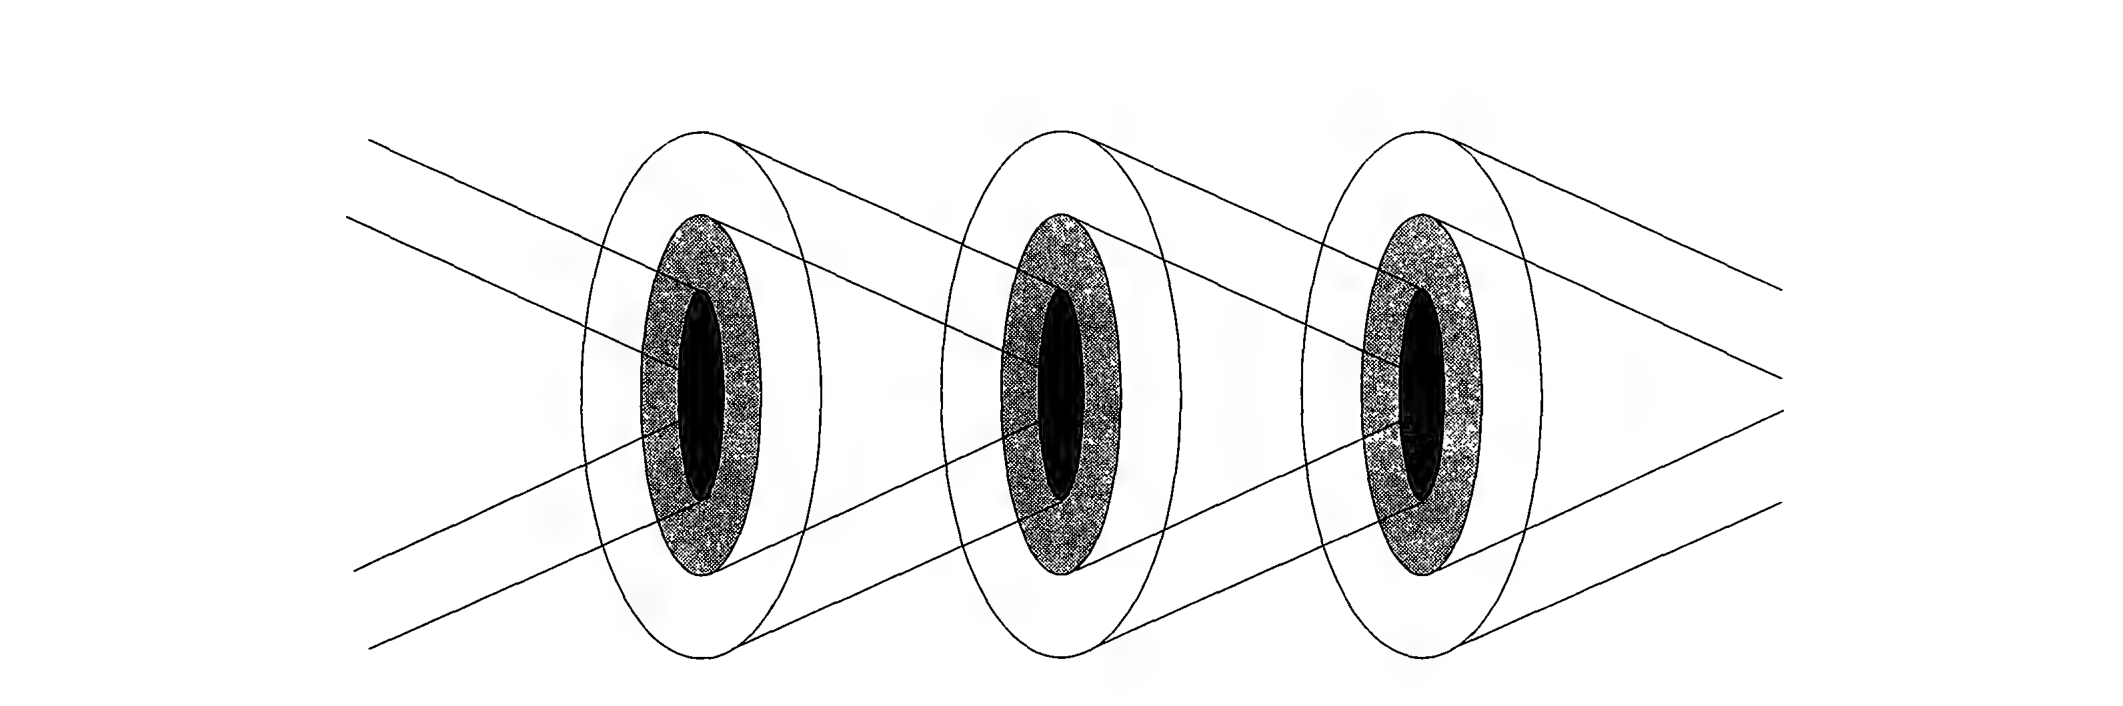
\includegraphics[width=0.88\textwidth]{figs/complex-heuristic.png}
\end{center}

椭圆是模 $M_i$; 黑色胖点是 $0$ 元素; 灰色椭圆在每一步被压扁到零, 它们是核; 由此我们形象地看到``前一个同态''的像落在``下一个同态''的核之内.

这幅图画并不精确之处在于: 它暗示 $d_{i+1}$ 的像与 $d_i$ 的核之间的``差'' (即着色较浅的灰色区域) 对所有的 $i$ 都相同; 当然一般情形并非如此. 事实上, 关于复形的几乎全部要点, 恰恰就是去``度量''这个差, 它被称为复形的同调%
\index{tongtiao@同调(homology)}
(参见 \S\ref{subsec:snake-lemma}). 若复形在``$M_i$ 处''没有同调, 我们就说它``在 $M_i$ 处''正合; 也就是说,
\[
\Image d_{i+1} = \Ker d_i.
\]
直观上看,
\begin{center}
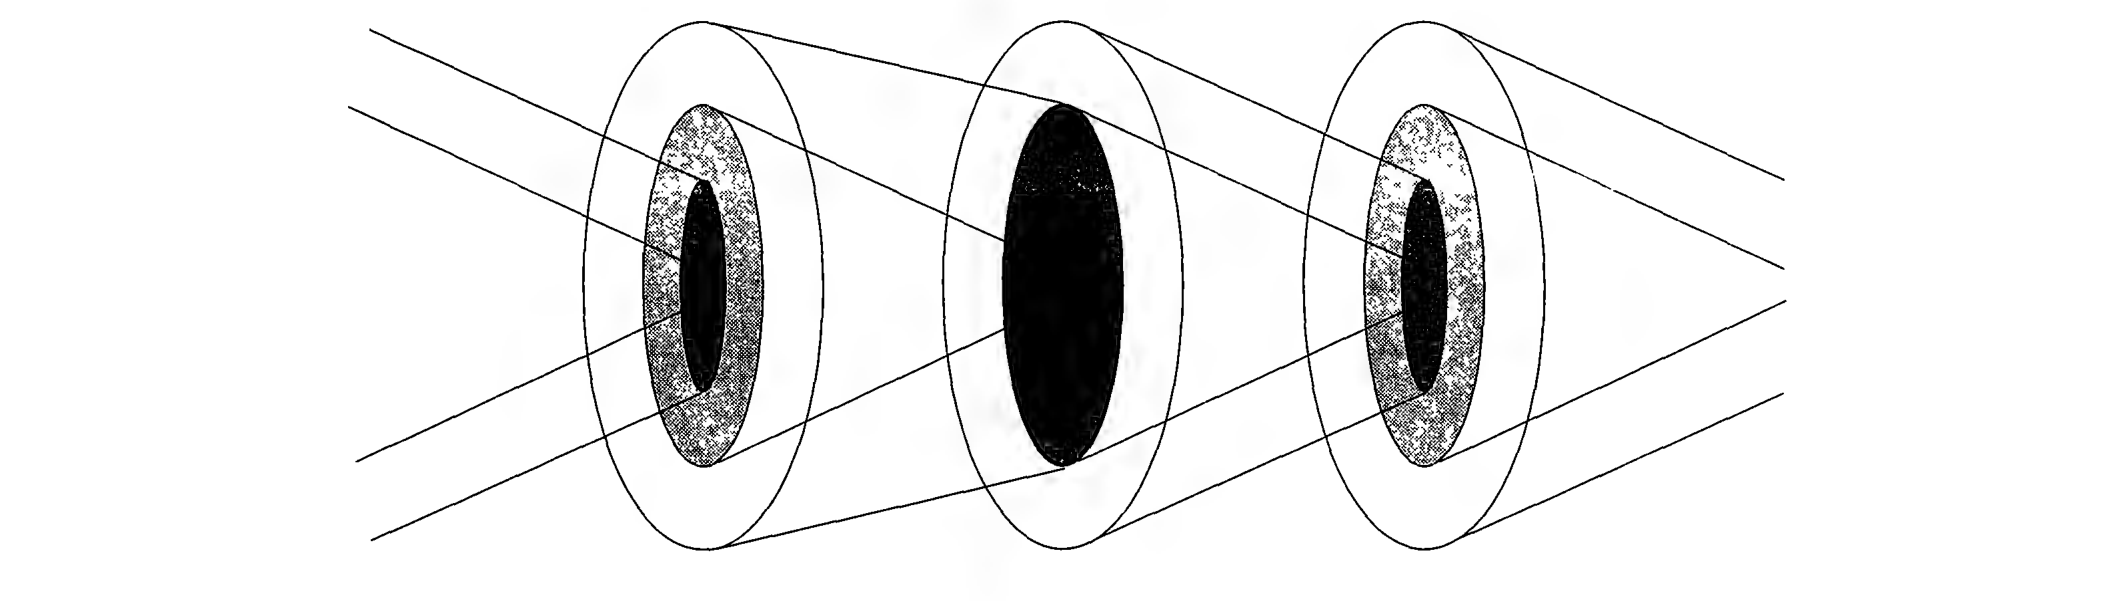
\includegraphics[width=0.88\textwidth]{figs/complex-exact.png}
\end{center}
这个复形看起来在中间那个椭圆处正合.

比如, 若 $M_i$ 是平凡模 (通常简单地记作 $0$), 则该复形必然在 $M_i$ 处正合, 因为此时 $\Image d_{i+1} = \Ker d_i = 0$.

若复形在它的所有模处都正合, 则称它是正合的, 并常被称为正合列%
\index{zhenghelie@正合列(exact sequence)}
.

\begin{example}
\label{ex:exact-mono}
复形
\[
\dots \longrightarrow 0 \longrightarrow L \xrightarrow{\ \alpha\ } M \longrightarrow \dots
\]
在 $L$ 处正合, 当且仅当 $\alpha$ 是单态射.

的确, 在 $L$ 处的正合等价于 $\Ker \alpha$ 等于平凡同态 $0 \to L$ 的像, 也就是说, 等价于
\[
\Ker \alpha = 0.
\]
这等价于 $\alpha$ 的单性 (命题~\ref{prop:mod-ker-coker}).
\end{example}

\begin{example}
\label{ex:exact-epi}
复形
\[
\dots \longrightarrow M \xrightarrow{\ \beta\ } N \longrightarrow 0 \longrightarrow \dots
\]
在 $N$ 处正合, 当且仅当 $\beta$ 是满态射.

的确, 该复形在 $N$ 处正合, 当且仅当 $\Image \beta$ 等于平凡同态 $N \to 0$ 的核, 也就是说, $\Image \beta = N$.
\end{example}

\begin{definition}
\label{def:short-exact}
短正合列%
\index{duanzhenghelie@短正合列(short exact sequence)}
是形如下式的正合复形:
\[
0 \longrightarrow L \xrightarrow{\ \alpha\ } M \xrightarrow{\ \beta\ } N \longrightarrow 0.
\]
\end{definition}

如前两例所见, 在 $L$ 与 $N$ 处的正合等价于 $\alpha$ 单、$\beta$ 满. 短正合列额外携带的信息是在 $M$ 处的正合, 也就是说,
\[
\Image \alpha = \Ker \beta;
\]
由第一同构定理 (推论~\ref{cor:module-first-iso}), 我们随之有
\[
N \cong \frac{M}{\Ker \beta} = \frac{M}{\Image \alpha}.
\]

总而言之, 我们手里有了进行更多巴甫洛夫式条件反射的好材料: 一看到上面那样的短正合列, 读者就应当本能地把 $L$ 认同为 $M$ 的子模 (经由单射 $\alpha$), 把 $N$ 认同为商 $M/L$ (经由满射 $\beta$ 在第一同构定理的庇护下诱导的同构).

短正合列在自然界中比比皆是. 比如, 单个同态 $\varphi : M \to M'$ 立即给出一个短正合列
\[
0 \longrightarrow \Ker \varphi \longrightarrow M \longrightarrow \Image \varphi \longrightarrow 0.
\]
事实上, 聚焦于短正合列的一个重要理由是: 这一观察使我们能够把每个正合复形打碎成大量的短正合列. 请欣赏这幅壮观的图:
\begin{center}
\begin{tikzcd}[column sep={4.4em,between origins}, row sep={2.3em,between origins}]
	&& 0 \ar[dr] && 0 && \\
	&&& \Image d_{i+1} = \Ker d_i \ar[ur] \ar[dr] &&& \\
	M_{i+2} \ar[rr, "d_{i+2}"] \ar[dr] && M_{i+1} \ar[rr, "d_{i+1}"] \ar[ur] && M_i \ar[rr, "d_i"] \ar[dr] && M_{i-1} \\
	& \Image d_{i+2} = \Ker d_{i+1} \ar[ur] \ar[dr] &&&& \Image d_i = \Ker d_{i-1} \ar[ur] \ar[dr] && \\
	0 \ar[ur] && 0 && 0 \ar[ur] && 0
\end{tikzcd}
\end{center}
斜向的序列是短正合列, 并且它们借助水平复形的正合性漂亮地互相咬合.

这一观察简化了许多论证; 参见例如习题~\ref{ex:noetherian-middle}.

\subsection{分裂正合列}
\label{subsec:split-exact}

短正合列的一种特殊情形, 来自考虑直和上的第二个投射: $M_1 \oplus M_2 \to M_2$; 于是有正合列
\[
0 \longrightarrow M_1 \longrightarrow M_1 \oplus M_2 \longrightarrow M_2 \longrightarrow 0,
\]
它通过把 $M_1$ 认同为该投射的核而得到. 这些短正合列被称为``分裂''的; 更一般地, 短正合列
\[
0 \longrightarrow M_1 \longrightarrow N \longrightarrow M_2 \longrightarrow 0
\]
称为``分裂''的, 如果它与上述序列之一同构, 意思是存在交换图
\begin{center}
\begin{tikzcd}
	0 \ar[r] & M_1 \ar[r] \ar[d, "\sim"'] & N \ar[r] \ar[d, "\sim"'] & M_2 \ar[r] \ar[d, "\sim"'] & 0 \\
	0 \ar[r] & M_1 \ar[r] & M_1 \oplus M_2 \ar[r] & M_2 \ar[r] & 0
\end{tikzcd}
\end{center}
其中竖直映射都是同构%
\footnote{事实上, 这最后一条要求有些多余; 参见习题~\ref{ex:extension-splits}.}%
.

\begin{example}
\label{ex:not-split}
$\Z$-模的正合列
\[
0 \longrightarrow \Z \xrightarrow{\ \cdot 2\ } \Z \longrightarrow \frac{\Z}{2\Z} \longrightarrow 0
\]
不分裂.
\end{example}

分裂序列给了我们一个机会, 回到 \S\ref{subsec:mod-ker-coker} 末尾悬而未决的问题: 对一个同态而言,``有左 (相应地, 右) 逆''这个条件应当怎么理解? 我们已经意识到这个条件比成为单态射\erratumfootnote{根据官方勘误, 原书英文此处将复数 monomorphisms 修正为单数 monomorphism.} (相应地, 满态射) 的要求更强; 我们能对这些态射给出更显式的描述吗?

\begin{proposition}
\label{prop:split-mono-epi}
设 $\varphi : M \to N$ 是 $R$-模同态. 那么
\begin{itemize}
	\item $\varphi$ 有左逆, 当且仅当序列
	\[
	0 \longrightarrow M \xrightarrow{\ \varphi\ } N \longrightarrow \Coker \varphi \longrightarrow 0
	\]
	分裂;
	\item $\varphi$ 有右逆, 当且仅当序列
	\[
	0 \longrightarrow \Ker \varphi \longrightarrow M \xrightarrow{\ \varphi\ } N \longrightarrow 0
	\]
	分裂.
\end{itemize}
\end{proposition}

\begin{proof}
我们证明第一部分, 另一部分作为练习留给读者 (习题~\ref{ex:split-epi}).

若序列分裂, 则可以把 $\varphi$ 认同为 $M$ 嵌入直和 $M \oplus M'$, 而投射 $M \oplus M' \to M$ 给出 $\varphi$ 的一个左逆. 反之, 设 $\varphi$ 有左逆 $\psi$:
\begin{center}
\begin{tikzcd}
	0 \ar[r] & M \ar[r,"\varphi"] \ar[dr,"\id_M"'] & N \ar[d,"\psi"] \\
& & M
\end{tikzcd}
\end{center}
那么我们断言: $N$ 同构于 $M \oplus \Ker \psi$, 且 $\varphi$ 对应于把 $M$ 认同第一因子: $M \to M \oplus \Ker \psi \cong N$. 同构 $M \oplus \Ker \psi \to N$ 由
\[
(m, k) \mapsto \varphi(m) + k
\]
给出; 它的逆 $N \to M \oplus \Ker \psi$ 是
\[
n \mapsto (\psi(n),\ n - \varphi\psi(n)).
\]
元素 $n - \varphi\psi(n)$ 在 $\Ker \psi$ 中, 理应如此, 因为
\[
\psi(n - \varphi\psi(n)) = \psi(n) - \psi\varphi\psi(n) = \psi(n) - \psi(n) = 0.
\]
所有必要的验证都是立即可得的, 留给读者.
\end{proof}

由于命题~\ref{prop:split-mono-epi}, 有左逆的 $R$-模同态称为分裂单态射%
\index{fenlidan@分裂单态射(split monomorphism)}
\index{fenlie@分裂(split)!yu@域(field)}, 有右逆的同态称为分裂满态射%
\index{fenliman@分裂满态射(split epimorphism)}
.

我们将在 \S IV.\ref{subsec:exact-sequences} (在要求更高的 $\cate{Grp}$ 语境中) 重回分裂正合列, 之后在我们回到模、以及更一般地回到 Abel 范畴 (第八与第九章) 时还会再遇到它们.

\subsection{同调与蛇形引理}
\label{subsec:snake-lemma}

\begin{definition}
\label{def:homology}
$R$-模的复形
\[
M_{\bullet}: \dots \xrightarrow{d_{i+2}} M_{i+1} \xrightarrow{d_{i+1}} M_i \xrightarrow{d_i} M_{i-1} \xrightarrow{d_{i-1}} \dots
\]
的第 $i$ 个同调是 $R$-模
\[
H_i(M_{\bullet}) := \frac{\Ker d_i}{\Image d_{i+1}}.
\]
\end{definition}

也就是说, $H_i(M_{\bullet})$ 是一个捕捉复形的启发式图像中``浅灰色环带''的模. 当然
\[
H_i(M_{\bullet}) = 0 \iff \Image d_{i+1} = \Ker d_i \iff \text{复形 } M_{\bullet} \text{ 在 } M_i \text{ 处正合}:
\]
也就是说, 同调模是``复形偏离正合的程度''的一种度量.

\begin{example}
\label{ex:homology-ker-coker}
事实上, 同调应当被想成核与余核这两个概念的 (宏伟的) 推广. 的确, 考虑 (非常) 特殊的情形: $M_{\bullet}$ 是复形
\[
0 \longrightarrow M_1 \xrightarrow{\ \varphi\ } M_0 \longrightarrow 0.
\]
那么
\[
H_1(M_{\bullet}) \cong \Ker \varphi, \qquad H_0(M_{\bullet}) \cong \Coker \varphi.
\]
\end{example}

我们将以指出一个涉及两个短正合列的交换图如何在同调中生成``长正合列''来结束这次对更抽象疆域的短暂访问. 这其实是更一般构造的特殊情形---按照那个构造, 一个涉及三个复形的适当交换图会产生一个真正长的``长正合同调列''. 当我们在第九章更深入地处理同调代数时, 会回到这个一般构造. 读者也很可能在代数拓扑的课程中学到它, 在那里这一事实被令人叹为观止地用于研究流形的不变量.

在我们要分析的简单形式中, 它被亲切地称为蛇形引理%
\index{shexingyinli@蛇形引理(snake lemma)}
. 考虑由同态相连的两个短正合列, 使它们构成交换图%
\footnote{事实上, 最好把这个图看作三个 (非常短的) 复形, 由 $R$-模同态 $\alpha_i$, $\beta_i$ 相连, 使得``行是正合的''. 其实, 人们可以定义复形的范畴, 而这个图不过是一个``复形的短正合列''; 这正是我们将在第九章采取的观点.}%
:
\begin{center}
\begin{tikzcd}[row sep=2.6em, column sep=2.6em]
	0 \ar[r] & L_1 \ar[r, "\alpha_1"] \ar[d, "\lambda"'] & M_1 \ar[r, "\beta_1"] \ar[d, "\mu"'] & N_1 \ar[r] \ar[d, "\nu"'] & 0 \\
	0 \ar[r] & L_0 \ar[r, "\alpha_0"'] & M_0 \ar[r, "\beta_0"'] & N_0 \ar[r] & 0
\end{tikzcd}
\end{center}

\begin{lemma}[蛇形引理]
\label{lem:snake}
沿用上图记号, 存在正合列
\[
0 \longrightarrow \Ker \lambda \longrightarrow \Ker \mu \longrightarrow \Ker \nu \xrightarrow{\ \delta\ } \Coker \lambda \longrightarrow \Coker \mu \longrightarrow \Coker \nu \longrightarrow 0.
\]
\end{lemma}

\begin{remark}
\label{rem:snake-induced}
该序列中的大多数同态都以完全直截了当的方式由相应的同态 $\lambda$, $\mu$, $\nu$ 诱导. 唯一``出人意料''的同态是记作 $\delta$ 的那一个; 我们将在下文讨论它的定义.
\end{remark}

\begin{remark}
\label{rem:snake-homology}
鉴于例~\ref{ex:homology-ker-coker}, 我们本可以把该陈述中的序列写成
\[
\begin{tikzcd}[column sep=1.4em,row sep=2.6em]
0 \ar[r] & H_1(L_\bullet) \ar[r] & H_1(M_\bullet) \ar[r] & H_1(N_\bullet) \ar[dlll,out=0,in=180,looseness=1.3,"\delta" description] \\
H_0(L_\bullet) \ar[r] & H_0(M_\bullet) \ar[r] & H_0(N_\bullet) \ar[r] & 0
\end{tikzcd}
\]
其中 $L_{\bullet}$ 是复形 $0 \longrightarrow L_1 \xrightarrow{\ \lambda\ } L_0 \longrightarrow 0$, 等等. 蛇形引理可以推广到任意复形 $L_{\bullet}$, $M_{\bullet}$, $N_{\bullet}$, 产生一个``长正合同调列'', 上式不过是它的尾端. 如上所述, 我们稍后会 (\S IX.\ref{subsec:3.3-les}) 讨论这个相当直截了当的推广.
\end{remark}

\begin{remark}
\label{rem:snake-general}
蛇形引理的一个流行版本不假定 $\alpha_1$ 单、$\beta_0$ 满: 也就是说, 我们可以考虑正合列的交换图
\begin{center}
\begin{tikzcd}[row sep=2.6em, column sep=2.6em]
	& L_1 \ar[r, "\alpha_1"] \ar[d, "\lambda"] & M_1 \ar[r, "\beta_1"] \ar[d, "\mu"] & N_1 \ar[r] \ar[d, "\nu"] & 0 \\
	0 \ar[r] & L_0 \ar[r, "\alpha_0"] & M_0 \ar[r, "\beta_0"] & N_0
\end{tikzcd}
\end{center}
此时引理将陈述: 存在``仅有的''正合列
\[
\Ker \lambda \longrightarrow \Ker \mu \longrightarrow \Ker \nu \xrightarrow{\ \delta\ } \Coker \lambda \longrightarrow \Coker \mu \longrightarrow \Coker \nu.
\]
\end{remark}

证明蛇形引理是一件不应当当众进行的事情, 而且把验证的细节写下来给别人看是出了名地无用: 那些细节本质上全都是显然的, 却会很快把人拖入记号的泥沼. 这类证明被统称为追图%
\index{zhuitu@追图(diagram chase)}
\index{gen@根(radical)!de@的(of)}的运动, 最佳的进行方式是: 在黑板上用几根手指同时指点图的不同部位, 一边念叨所摆弄的元素, 一边宣布它们的命运%
\footnote{真正的纯粹主义者会在任意范畴中追图, 从而没有谈论``元素''的便利; 我们稍后 (第九章) 会练习这项技能. 比如, 蛇形引理可以靠一个接一个地诉诸核与余核的万有性质来证明, 自始至终不选取任何元素. 但对着黑板指指点点、自言自语地过完论证的表演技巧, 本质上还是那一套.}%
.

尽管如此, 我们还是应当解释``连接''同态 $\delta$ 从何而来, 因为它是蛇形引理的陈述及其证明的核心. 这是包含核与余核的整幅图; 于是, 列是正合的 (连同水平放置的两条原序列也正合):
\begin{center}
\begin{tikzcd}[
row sep=1.2cm, column sep=1.2cm,
% 注意: execute at end picture 的大括号内绝对不能有“空行”, 否则会报 Runaway argument 错误！
execute at end picture={
\coordinate (p1) at ($(kg.east) + (2, 0)$);
\coordinate (mid) at ($(B.south)!0.55!(Bp.north)$);
\coordinate (p2) at (p1 |- mid);
\coordinate (p4) at ($(ca.west) - (2, 0)$);
\coordinate (p3) at (p4 |- p2);
\draw[->, rounded corners=12pt, thick, preaction={draw, white, line width=4pt}]
(kg.east) -- (p1) -- node[right] {$\delta$} (p2) -- (p3) -- (p4) -- (ca.west);
}
]
% 第 1 行
& 0 \arrow[d] & 0 \arrow[d] & 0 \arrow[d] & \\
% 第 2 行
0 \arrow[r] & \Ker\lambda \arrow[d] \arrow[r] & \Ker\mu \arrow[d] \arrow[r] & |[alias=kg]| \Ker\nu \arrow[d] & \\
% 第 3 行
0 \arrow[r] & L_1 \arrow[d, "\lambda" near start] \arrow[r, "\alpha_1"] & |[alias=B]| M_1 \arrow[d, "\mu" near start] \arrow[r, "\beta_1"] & N_1 \arrow[d, "\nu" near start] \arrow[r] & 0 \\
% 第 4 行
0 \arrow[r] & L_0 \arrow[d] \arrow[r, "\alpha_0"'] & |[alias=Bp]| M_0 \arrow[d] \arrow[r, "\beta_0"'] & N_0 \arrow[d] \arrow[r] & 0 \\
% 第 5 行
& |[alias=ca]| \Coker\lambda \arrow[d] \arrow[r] & \Coker\mu \arrow[d] \arrow[r] & \Coker\nu \arrow[d] \arrow[r] & 0 \\
% 第 6 行
& 0 & 0 & 0 &
\end{tikzcd}
\end{center}
顺便说, 我们相信读者现在明白了这条引理为何得名``蛇形''.

蛇形同态 $\delta$ 的定义. 设 $a \in \Ker \nu$. 我们断言: $a$ 可以沿着图中标记的实线箭头一路穿越到 $\Coker \lambda$:
\begin{center}
\begin{tikzcd}[row sep=1.6em,column sep=1.9em]
& 0 \ar[d,dotted,no head] & 0 \ar[d,dotted,no head] & 0 \ar[d,dotted,no head] & \\
0 \ar[r,dotted,no head] & \vphantom{e} \ar[r,dotted,no head] \ar[d,dotted,no head] & \vphantom{c} \ar[r,dotted,no head] \ar[d,dotted,no head] & a \ar[d] & \\
0 \ar[r,dotted,no head] & \vphantom{e} \ar[r,dotted,no head] \ar[d,dotted,no head] & c \ar[r,"\beta_1"] \ar[d,"\mu"] & b \ar[r,dotted,no head] \ar[d,dotted,no head,"\nu"] & 0 \\
0 \ar[r,dotted,no head] & e \ar[r,"\alpha_0"'] \ar[d] & d \ar[r,dotted,no head,"\beta_0"'] \ar[d,dotted,no head] & * \ar[r,dotted,no head] \ar[d,dotted,no head] & 0 \\
& f \ar[r,dotted,no head] \ar[d,dotted,no head] & \vphantom{f} \ar[r,dotted,no head] \ar[d,dotted,no head] & \vphantom{f} \ar[r,dotted,no head] \ar[d,dotted,no head] & 0 \\
& 0 & 0 & 0 &
\end{tikzcd}
\end{center}
的确,
\begin{itemize}
	\item $\Ker \nu \subseteq N_1$; 于是把 $a$ 视为 $N_1$ 的元素 $b$;
	\item $\beta_1$ 是满的, 故存在 $c \in M_1$ 映到 $b$;
	\item 令 $d = \mu(c)$ 为 $c$ 在 $M_0$ 中的像;
	\item $d$ 在标记 $*$ 的位置上的像是什么? 由图的交换性, 它必与 $\nu(b)$ 相同. 然而 $b$ 是 $a \in \Ker \nu$ 在 $N_1$ 中的像, 故 $\nu(b) = 0$. 于是 $d \in \Ker \beta_0$. 由于行正合, $\Ker \beta_0 = \Image \alpha_0$; 因此存在 $e \in L_0$ 映到 $d$;
	\item 最后, 令 $f \in \Coker \lambda$ 为 $e$ 的像.
\end{itemize}
我们想规定 $\delta(a) := f$.

这样做合法吗? 在追图的两步中我们取了原像:
\begin{itemize}
	\item 存在 $c \in M_1$ 使 $\beta_1(c) = b$;
	\item 存在 $e \in L_0$ 使 $\alpha_0(e) = d$.
\end{itemize}
第二步不涉及选择: 由于按假设 $\alpha_0$ 是单射, 映到 $d$ 的元素 $e$ 由 $d$ 唯一决定. 但第一步涉及选择: 为了验证 $\delta$ 是良定义的, 我们必须证明选取别的 $c$ 不会影响为 $\delta(a)$ 提议的值 $f$.

这要用另一次追图来证明. 图中相关的部分是:
\begin{center}
\begin{tikzcd}[row sep=2em,column sep=2em]
0 \ar[r,dotted,no head] & \vphantom{g} \ar[r,dotted,no head,"\alpha_1"] \ar[d,dotted,no head,"\lambda"'] & c \ar[r,"\beta_1"] \ar[d,"\mu"] & b \ar[r,dotted,no head] \ar[d,dotted,no head] & 0 \\
0 \ar[r,dotted,no head] & e \ar[r,"\alpha_0"'] \ar[d] & d \ar[r,dotted,no head] \ar[d,dotted,no head] & \vphantom{d} & \\
& f \ar[r,dotted,no head] & \vphantom{f} & &
\end{tikzcd}
\end{center}
假设我们选取映射到同一个 $b$ 的另一个 $c'$:
\[
\begin{tikzcd}
0 \ar[r,dotted,no head] & \vphantom{g} \ar[r,dotted,no head,"\alpha_1"] & c' \ar[r,"\beta_1"] & b \ar[r,dotted,no head] & 0
\end{tikzcd}.
\]
那么 $\beta_1(c' - c) = 0$; 由正合性, 存在 $g \in L_1$ 使 $(c' - c) = \alpha_1(g)$:
\[
g \xrightarrow{\ \alpha_1\ } (c' - c) \xrightarrow{\ \beta_1\ } 0.
\]
现在的要点是: 由于列构成复形, $g$ 在 $\Coker \lambda$ 中死去:
\[
\begin{tikzcd}[column sep=small]
0 \ar[r,dotted,no head] & g \ar[r,"\alpha_1"] \ar[d,"\lambda"'] & c'-c \ar[r,"\beta_1"] \ar[d,"\mu"] & 0 \\
0 \ar[r,dotted,no head] & \lambda(g) \ar[r,dotted,no head,"\alpha_0"] \ar[d] & \vphantom{d} \ar[r,dotted,no head] \ar[d,dotted,no head] & \vphantom{0} \\
& 0 \ar[r,dotted,no head] & \vphantom{f} &
\end{tikzcd}
\]
于是 (由图的交换性与 $\alpha_0$ 的单性) 得知: 把 $c$ 换成 $c'$ 会把 $e$ 修改为 $e + \lambda(g)$, 把 $f$ 修改为 $f + 0 = f$. 也就是说, $f$ 的确与选取无关.

于是 $\delta$ 是良定义的!

这只是蛇形引理证明的极小的一部分, 但大概足以说明为什么阅读写出来的追图过程可能极其缺乏信息量.

证明的其余部分 (留给读者 (!); 我们没有把它列为正式习题, 唯恐真有人交来一份作业等待评分) 由许许多多类似的论证组成. 在核与余核上诱导的映射的定义, 比上面描述的连接态射 $\delta$ 的定义要容易得多. 序列
\[
0 \longrightarrow \Ker \lambda \longrightarrow \Ker \mu \longrightarrow \Ker \nu \xrightarrow{\ \delta\ } \Coker \lambda \longrightarrow \Coker \mu \longrightarrow \Coker \nu \longrightarrow 0
\]
在大多数位置的正合性也相当直截了当; 大部分工作将花在证明在 $\Ker \nu$ 与 $\Coker \lambda$ 处的正合性上.

亲爱的读者: 不要回避尝试, 因为这是极好且不可或缺的练习. 错过这次机会, 你将永远对这类操作心中无底.

蛇形引理把若干个事实串成一线, 这些事实单独证明并不困难, 但引理一旦落定它们就变得真正直截了当. 比如,

\begin{corollary}
\label{cor:short-five}
在与蛇形引理相同的情形中 (记号同 \S\ref{subsec:snake-lemma}), 设 $\mu$ 是满的且 $\nu$ 是单的. 则 $\lambda$ 是满的, 且 $\nu$ 是同构.
\end{corollary}

\begin{proof}
的确, $\mu$ 满 $\implies \Coker \mu = 0$; $\nu$ 单 $\implies \Ker \nu = 0$ (命题~\ref{prop:mod-ker-coker}). 把这些信息输入蛇形引理的序列, 得到正合列
\[
0 \longrightarrow \Ker \lambda \longrightarrow \Ker \mu \longrightarrow 0 \longrightarrow \Coker \lambda \longrightarrow 0 \longrightarrow \Coker \nu \longrightarrow 0.
\]
正合性蕴含 $\Coker \lambda = \Coker \nu = 0$ (习题~\ref{ex:exact-zero}); 故 $\lambda$ 与 $\nu$ 是满的, 得到所述结论.
\end{proof}

还有几个这类陈述可以同样轻松地证明; 读者尽可随心所欲地试验.

\subsection*{习题}
\phantomsection
\addcontentsline{toc}{subsection}{习题}

\begin{prob}
\label{ex:exact-zero}
$\triangleright$ 设复形
\[
\dots \longrightarrow 0 \longrightarrow M \longrightarrow 0 \longrightarrow \dots
\]
正合. 证明 $M \cong 0$. [\S\ref{subsec:snake-lemma}]
\end{prob}

\begin{prob}
\label{ex:exact-iso}
设复形
\[
\dots \longrightarrow 0 \longrightarrow M \longrightarrow M' \longrightarrow 0 \longrightarrow \dots
\]
正合. 证明 $M \cong M'$.
\end{prob}

\begin{prob}
\label{ex:ker-coker-exact}
设复形
\[
\dots \longrightarrow 0 \longrightarrow L \longrightarrow M \xrightarrow{\ \varphi\ } M' \longrightarrow N \longrightarrow 0 \longrightarrow \dots
\]
正合. 证明: 在相差自然认同的意义下, $L = \Ker \varphi$ 且 $N = \Coker \varphi$.
\end{prob}

\begin{prob}
\label{ex:Hilbert-hotel}
构造 $\Z$-模的短正合列
\[
0 \longrightarrow \Z^{\oplus \N} \longrightarrow \Z^{\oplus \N} \longrightarrow \Z \longrightarrow 0
\]
与
\[
0 \longrightarrow \Z^{\oplus \N} \longrightarrow \Z^{\oplus \N} \longrightarrow \Z^{\oplus \N} \longrightarrow 0.
\]
(提示: David Hilbert 的大旅馆.)
\end{prob}

\begin{prob}
\label{ex:noetherian-middle}
$\triangleright$ 设复形
\[
\dots \longrightarrow L \longrightarrow M \longrightarrow N \longrightarrow \dots
\]
正合, 且 $L$ 与 $N$ 是 Noether 的. 证明 $M$ 是 Noether 的. [\S\ref{subsec:complexes}]
\end{prob}

\begin{prob}
\label{ex:split-epi}
$\triangleright$ 证明命题~\ref{prop:split-mono-epi} 的``分裂满态射''部分. [\S\ref{subsec:split-exact}]
\end{prob}

\begin{prob}
\label{ex:hom-left-exact}
$\triangleright$ 设
\[
0 \longrightarrow M \longrightarrow N \longrightarrow P \longrightarrow 0
\]
是 $R$-模的短正合列, $L$ 是 $R$-模.
\begin{itemize}
	\item[(i)] 证明存在正合列%
	\footnote{一般地, 这将是 Abel 群的序列; 若 $R$ 交换, 从而每个 $\Hom_{R\dcate{Mod}}$ 都是 $R$-模 (\S\ref{subsec:R-Mod-hom}), 则它将是 $R$-模的正合列.}
	\[
	0 \longrightarrow \Hom_{R\dcate{Mod}}(P, L) \longrightarrow \Hom_{R\dcate{Mod}}(N, L) \longrightarrow \Hom_{R\dcate{Mod}}(M, L).
	\]
	\item[(ii)] 重做习题~\ref{ex:hom-cyclic}. (用正合列 $0 \to I \to R \to R/I \to 0$.)
	\item[(iii)] 构造一个例子, 表明 (i) 中最右边的同态不必是满的.
	\item[(iv)] 证明: 若原序列分裂, 则 (i) 中最右边的同态是满的.
\end{itemize}
[\ref{ex:free-hom-exact}, VIII.\ref{ex:quotient-base-change}, \S~VIII.\ref{subsec:hom-adjunction-again}]
\end{prob}

\begin{prob}
\label{ex:free-splits}
$\triangleright$ 证明: $R$-模的每个正合列
\[
0 \longrightarrow M \longrightarrow N \longrightarrow F \longrightarrow 0,
\]
其中 $F$ 自由, 都分裂. (提示: 习题~\ref{ex:projective-free}.) [\S~VIII.\ref{subsec:duality-exactness}]
\end{prob}

\begin{prob}
\label{ex:free-hom-exact}
设
\[
0 \longrightarrow M \longrightarrow N \longrightarrow F \longrightarrow 0
\]
是 $R$-模的短正合列, $F$ 自由, $L$ 是 $R$-模. 证明存在正合列
\[
0 \longrightarrow \Hom_{R\dcate{Mod}}(F, L) \longrightarrow \Hom_{R\dcate{Mod}}(N, L) \longrightarrow \Hom_{R\dcate{Mod}}(M, L) \longrightarrow 0.
\]
(参见习题~\ref{ex:hom-left-exact}.)
\end{prob}

\begin{prob}
\label{ex:short-five}
\index{youxiankefenkuozhangshijiandande@有限可分扩张是简单的(finite separable extensions are simple)!wuyinli@五引理(five-lemma)!duan@短(short)}\index{youxiankefenkuozhangshijiandande@有限可分扩张是简单的(finite separable extensions are simple)!wuyinli@五引理(five-lemma)}$\triangleright$ 在蛇形引理的情形中, 设 $\lambda$ 与 $\nu$ 是同构. 用蛇形引理证明 $\mu$ 是同构. 它被称为``短五引理'', 因为它立即由五引理 (参见习题~\ref{ex:five-lemma}) 推出, 也由蛇形引理推出. [VIII.\ref{ex:ext-extensions}, IX.\ref{ex:2.4}]
\end{prob}

\begin{prob}
\label{ex:extension-splits}
$\triangleright$ 设
\begin{equation*}
0 \longrightarrow M_1 \longrightarrow N \longrightarrow M_2 \longrightarrow 0 \tag{$*$}
\end{equation*}
是 $R$-模的正合列. (它可以称为 $M_2$ 被 $M_1$ 扩张所得的一个``扩充''.) 设存在任意一个使图
\[
\begin{tikzcd}[column sep=small]
0 \ar[r] & M_1 \ar[r] \ar[d,equal] & N \ar[r] \ar[d,dashed] & M_2 \ar[r] \ar[d,equal] & 0 \\
0 \ar[r] & M_1 \ar[r] & M_1\oplus M_2 \ar[r] & M_2 \ar[r] & 0
\end{tikzcd}
\]
交换的 $R$-模同态 $N \to M_1 \oplus M_2$, 其中下方的序列是直和的标准序列. 证明 $(*)$ 分裂. [\S\ref{subsec:split-exact}]
\end{prob}

\begin{prob}
\index{siyinli@四引理(four-lemma)}\label{ex:four-lemma}
$\neg$ 用证明``四引理''来练习你的追图技艺: 若
\[
\begin{tikzcd}[column sep=small]
A_1 \ar[r] \ar[d, "\alpha"'] & B_1 \ar[r] \ar[d, "\beta"'] & C_1 \ar[r] \ar[d, "\gamma"'] & D_1 \ar[d, "\delta"'] \\
A_0 \ar[r] & B_0 \ar[r] & C_0 \ar[r] & D_0
\end{tikzcd}
\]
是行为正合的 $R$-模交换图, $\alpha$ 是满态射, $\beta$ 与 $\delta$ 是单态射, 则 $\gamma$ 是单态射. [\ref{ex:four-lemma-2}, IX.\ref{ex:2.3}]
\end{prob}

\begin{prob}
\label{ex:four-lemma-2}
证明习题~\ref{ex:four-lemma} 的``四引理''的另一个%
\footnote{事实上, 两个版本不必都证明; 但要意识到这一点, 必须从 Abel 范畴这一更一般的语境来看待问题; 参见习题~IX.\ref{ex:2.3}.}%
版本: 若
\[
\begin{tikzcd}[column sep=small]
B_1 \ar[r] \ar[d, "\beta"'] & C_1 \ar[r] \ar[d, "\gamma"'] & D_1 \ar[r] \ar[d, "\delta"'] & E_1 \ar[d, "\epsilon"'] \\
B_0 \ar[r] & C_0 \ar[r] & D_0 \ar[r] & E_0
\end{tikzcd}
\]
是行为正合的 $R$-模交换图, $\beta$ 与 $\delta$ 是满态射, $\epsilon$ 是单态射, 则 $\gamma$ 是满态射.
\end{prob}

\begin{prob}
\label{ex:five-lemma}
$\neg$ 证明``五引理'': 若
\begin{center}
\begin{tikzcd}[row sep=2.2em, column sep=1.9em]
	A_1 \ar[r] \ar[d, "\alpha"'] & B_1 \ar[r] \ar[d, "\beta"'] & C_1 \ar[r] \ar[d, "\gamma"'] & D_1 \ar[r] \ar[d, "\delta"'] & E_1 \ar[d, "\epsilon"'] \\
	A_0 \ar[r] & B_0 \ar[r] & C_0 \ar[r] & D_0 \ar[r] & E_0
\end{tikzcd}
\end{center}
是行为正合的 $R$-模交换图, $\beta$ 与 $\delta$ 是同构, $\alpha$ 是满态射, $\epsilon$ 是单态射, 则 $\gamma$ 是同构. (把前面几道习题的结果拼接起来, 可以避免所需的追图.) [\ref{ex:short-five}]
\end{prob}

\begin{prob}
\index{jiuyinli@九引理(nine-lemma)}\label{ex:nine-lemma}
$\neg$ 考虑下面的 $R$-模交换图:
\begin{center}
\begin{tikzcd}[row sep=1.8em,column sep=1.9em]
&0 \ar[d] &0 \ar[d] &0 \ar[d] & \\
0 \ar[r] &L_2 \ar[r] \ar[d] &M_2 \ar[r] \ar[d,"\alpha"] &N_2 \ar[r] \ar[d] &0 \\
0 \ar[r] &L_1 \ar[r] \ar[d] &M_1 \ar[r] \ar[d,"\beta"] &N_1 \ar[r] \ar[d] &0 \\
0 \ar[r] &L_0 \ar[r] \ar[d] &M_0 \ar[r] \ar[d] &N_0 \ar[r] \ar[d] &0 \\
&0 &0 &0 &
\end{tikzcd}
\end{center}
设三行都正合, 且最右边的两列正合. 证明左列正合. 第二版本: 设三行都正合, 且最左边的两列正合; 证明右列正合. 这就是``九引理''. (对图作 $90^{\circ}$ 旋转后应用蛇形引理, 可以避免追图.) [\ref{ex:nine-lemma-2}]
\end{prob}

\begin{prob}
\label{ex:nine-lemma-2}
在与习题~\ref{ex:nine-lemma} 相同的情形中, 设三行都正合, 且最左列与最右列正合.
\begin{itemize}
	\item 证明 $\alpha$ 是单态射, $\beta$ 是满态射.
	\item 中间列必然正合吗?
\end{itemize}
(提示: 不必然. 把 $\Z \oplus \Z$ 放在中间, 并用六份 $\Z$ 与两个 $0$ 巧妙地围住它.)
再假定中央列是复形, 即 $\beta\circ\alpha=0$; 证明此时中央列必正合.
\end{prob}

\begin{prob}
\label{ex:infinite-nine-lemma}
$\neg$ 如下推广前两道习题. 考虑一个 (可能无限的) $R$-模交换图:
\[
\begin{tikzcd}[row sep=1.8em,column sep=2em]
&\vdots \ar[d] &\vdots \ar[d] &\vdots \ar[d] & \\
0 \ar[r] &L_{i+1} \ar[r] \ar[d] &M_{i+1} \ar[r] \ar[d] &N_{i+1} \ar[r] \ar[d] &0 \\
0 \ar[r] &L_i \ar[r] \ar[d] &M_i \ar[r] \ar[d] &N_i \ar[r] \ar[d] &0 \\
0 \ar[r] &L_{i-1} \ar[r] \ar[d] &M_{i-1} \ar[r] \ar[d] &N_{i-1} \ar[r] \ar[d] &0 \\
&\vdots &\vdots &\vdots &
\end{tikzcd}
\]
其中中央列是复形, 且每行都正合. 证明左列与右列也是复形. 证明任意两列正合时, 第三列也正合. (第一部分是直截了当的. 第二部分由于需要追图, 现在会花你几分钟; 等学过 \S~IX.\ref{subsec:3.3-les} 的长正合 (上) 同调列之后, 只需几秒钟.) [IX.\ref{ex:3.12}]
\end{prob}
